\documentclass[11pt]{article}

% Informations

% Modules 
\usepackage[greek,english]{babel}
\usepackage{graphicx}                       % Gestion des images
\usepackage{caption}                        % Gestion des titres
\usepackage{appendix}                       % Gestion de l'annexe
\usepackage[utf8]{inputenc}                 % Encodage du texte
\usepackage{multicol}                       % Gestion des multi-colonnes des tableaux
\usepackage{booktabs}                       % Importation des traits horizontaux des tableaux
\usepackage{siunitx}                        % Gestion des unités
\usepackage{mwe,lipsum}                     % Modules de Minimal Working Examples
\usepackage{amsmath,amssymb,amsbsy}         % Ajout d'options dans le mode 'math'
\usepackage{todonotes}                      % Ajout des notes en marge
\usepackage{mathtools}                      % Autres outils pour le mode 'math'
\usepackage{hyperref}            % Gestion des hyper-liens (internes et url)
\usepackage[a4paper]{geometry}                       % Options de mise en page
\usepackage{listings}
\usepackage{color,xcolor}
\usepackage{csquotes}
\usepackage{textcomp}
\usepackage{fancyhdr}
\usepackage[T1]{fontenc}
\usepackage{lato}
\usepackage{titling}
\usepackage{datetime}
\usepackage[version=4]{mhchem}
\usepackage{authblk}
\usepackage{enumitem}
\usepackage{tablefootnote}
\usepackage{cases}
\usepackage{bbm}
\usepackage{lmodern}
\usepackage{empheq}


\setitemize{itemsep=0pt}
\setcounter{MaxMatrixCols}{20}

% Police d'écriture
\renewcommand\familydefault{\sfdefault}

% Définition de couleurs
% \definecolor{Bleu_ENSPS}{RGB}{0,119,139}
\definecolor{CIRED_blue}{RGB}{6,100,110}
\hypersetup{
    hidelinks,
    }

% Options de biliographie 
\usepackage[style=authoryear,giveninits=true,sorting=nty,maxcitenames=1]{biblatex}
% \usepackage[backend=biber, bibstyle=ieee, citestyle=numeric-comp,
%   sorting=none, labeldateparts,
%   maxbibnames=99, maxcitenames=2, mincitenames=1]{biblatex} 
\DefineBibliographyExtras{french}{\restorecommand\mkbibnamefamily}

\AtEveryBibitem{%
  \clearlist{language}%
  \clearlist{urldate}
  \clearlist{url}
  \clearfield{month}
  \clearfield{day}
  \clearfield{note}
}
\DeclareFieldFormat{url}{}
\DeclareFieldFormat{urldate}{}

\DeclareFieldFormat{journaltitle}{\textit{#1}}
\DeclareFieldFormat{title}{#1}

\setlength\bibitemsep{\itemsep}
\AtEveryCite{\color{CIRED_blue}}

\addbibresource{/home/amounier/Documents/Bibliographie/bibliographie_bib.bib}
\bibliography{biblatex-examples.bib}

% All name in hyperlink (cite biblatex)
\makeatletter
\let\abx@macro@citeOrig\abx@macro@cite
\renewbibmacro{cite}{%
   \bibhyperref{%
   \let\bibhyperref\relax\relax%
   \abx@macro@citeOrig%
   }%
}
\let\abx@macro@textciteOrig\abx@macro@textcite
\renewbibmacro{textcite}{%
   \bibhyperref{%
   \let\bibhyperref\relax\relax%
   \abx@macro@textciteOrig%
   }%
}%
\makeatother

% Options de format pour les unités (SIUnitX package)
\sisetup{
    detect-all,
    locale                  = UK,
    sticky-per,
    inter-unit-product      = {.},
    per-mode                = reciprocal-positive-first,
}

\DeclareSIUnit\octet{o}
\DeclareSIUnit\watthour{Wh}
\DeclareSIUnit\year{yr}
\DeclareSIUnit\hab{inhab}

%Options de largeur de marges, verticales et horizontales
\geometry{hmargin=3cm,vmargin=2cm}
\setlength{\parindent}{7mm}

% Mise en page
% \pagestyle{fancy}
% \setlength{\headheight}{14pt}
% \renewcommand\headrulewidth{0.5pt}
% \renewcommand\footrulewidth{0.5pt}
% \fancyhead[C]{\thedate}
% \fancyhead[R]{}
% \fancyhead[L]{}
% \fancyhead[R]{\rightmark}

% Styles équations
%\numberwithin{equation}{section}

\makeatletter
\renewcommand\p@figure{Figure~\@ }
\makeatother

\makeatletter
\renewcommand\p@table{Table~\@ }
\makeatother

%Autres commandes
\addto\captionsfrench{
  \renewcommand{\contentsname}%
    {Sommaire}%
}

% Keywords command
\providecommand{\keywords}[1]
{
  \small    
  \textbf{\textit{Keywords~--}} #1
}

% \renewcommand{\paragraph}[1]{\paragraph{#1}\mbox{}\\}

% Titre ---------------------------------------
\date{\today}
\title{Interactions between summer and winter thermal comfort, effects of climate change on optimal renovation actions}

\author[1,3,4]{André Mounier}
\author[2,3]{Louis-Gaëtan Giraudet}
\author[4]{Philippe Drobinski}
\affil[1]{\small{Agence de l'environnement et de la maîtrise de l'énergie (ADEME), Angers, France}}
\affil[2]{\small{ENPC - Institut Polytechnique de Paris, Champs-sur-Marne, France}}
\affil[3]{\small{CIRED -- ENPC, AgroParisTech, EHESS, Cirad, CNRS, Nogent-sur-Marne, France}}
\affil[4]{\small{LMD -- IPSL, École Polytechnique - IPP, ENS - PSL , Sorbonne Université, CNRS, Palaiseau, France}}

\begin{document}


\maketitle

% Contenu -------------------------------------

% Méthode :
% https://www.nature.com/documents/nature-summary-paragraph.pdf
\begin{abstract}
    Energy efficiency building renovation, particularly through thermal insulation, is a key factor in the transformation of the building stock to reduce greenhouse gas emissions and adapt dwellings to future climates. Thermal renovation of buildings is a particularly costly operation that rarely pays off for the person carrying out the work. In France, many renovation projects are financed in part by the state, and this funding involves targeting the most effective works. However, this efficiency is only measured in terms of heating needs, while the critical nature of the inadequacy of housing for future heat increases year on year.  Taking account of climate change, its future evolution, and the need to adapt homes will therefore influence the optimum renovations to target as a priority now. Here we show that the displacement of the optimum differs according to the type of building and the intensity of warming, and according to the type of renovation work. This study presents a first way of considering dynamic, energy and economic optimisations, with RC modelling of building typologies. The conclusions are different depending on the type of action carried out: for example, the insulation of opaque walls does have an antagonistic effect on heating and cooling needs (but this is particularly visible in the coldest meteorological years and without night-time natural over-ventilation), but total energy needs are always decreasing. Thus, inter-annual variations in typology and weather play a decisive role in defining the optimum. The results call into question the selection criteria for subsidised renovations, as well as the renovations carried out in practice in France. The question of the interaction between summer and winter comfort has been raised in official reports in France, because adaptation is underdeveloped, and the majority of measures are focused on winter thermal comfort. A deliberately provocative question could be: ‘Do we need to renovate buildings on a massive scale if the French climate warms up significantly between now and the end of the century? The answer is yes, but not for all buildings or all regions in the same way. 
\end{abstract}

\keywords{Thermal insulation, Heating and cooling needs, Adaptation, Mitigation}

\clearpage
\tableofcontents

\clearpage

\section{Introduction}
\label{sec:intro}

consommations des batiments dans le monde et en France (\cite{unep_2023_2024}, \cite{sdes_chiffres_2023}, \cite{sdes_consommation_2023})

changement climatique en France (physique et scenarios officiels) (\cite{ipcc_climate_2021}, \cite{ouzeau_heat_2016}, \cite{ministere_de_la_transition_ecologique_trajectoire_2023})

consommations futures des batiments (\cite{larsen_climate_2020},\cite{moreau_evaluation_2023},\cite{filahi_projections_2024}, \cite{tao_uncertainty_2024})

inadaptation du parc aux temperatures futures (\cite{cour_des_comptes_laction_2024}, \cite{i4ce_vagues_2024})

rentabilité et cout des renovations (\cite{ademe_renovation_2019}, \cite{i4ce_trajectoires_2023}, \cite{giraudet_analyse_2024})

critères de soutiens aux travaux d'isolation (\cite{france_strategie_dispositif_2024}, \cite{coulaud_maprimerenov_2024}, \cite{anah_aides_2024-1})

\clearpage
\section{RC analogy modelling}
\label{sec:rc}

    \subsection{RC analogy and computation} % (fold)
    \label{sub:rc_analogy_and_computation}

        \subsubsection{RC analogy} % (fold)
        \label{ssub:rc_analogy}


        \cite{fourier_theorie_1822}, \cite{bolmont_evolution_2003}
        
        % subsubsection rc_analogy (end)

        \subsubsection{Model construction} % (fold)
        \label{ssub:model_construction}

        \paragraph{Simplified RC model}\mbox{}\\ % (fold)
        \label{par:simplified_rc_model}

        À but illustratif (\ref{fig:RClight})

        \begin{figure}[ht]
            \centering
            
\includegraphics[width=0.33\columnwidth]{figures/building.drawio.png}
            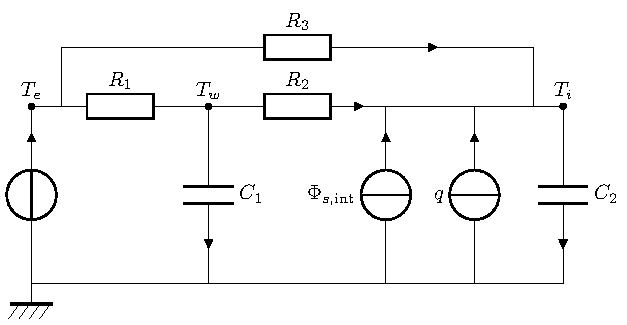
\includegraphics[width=0.66\columnwidth]{figures/R3C2.pdf}
            \caption{\label{fig:RClight} Diagram of a building and the associated simplified RC model}
            \begin{quote}
                \vspace{-2mm}
                \small\noindent
                Description.
            \end{quote}
         \end{figure}

        The RC model shown in the \ref{fig:RClight} provides a synthetic representation of the general model described below (\ref{par:general_rc_model}). The various thermal and energy variables represented are as follows:
        $$
        \begin{dcases}
          T_e&:\text{ External temprature (\SI{}{\celsius})} \\
          T_w&:\text{ Wall internal temperature (\SI{}{\celsius})} \\
          T_i&:\text{ Internal temperature (\SI{}{\celsius})} \\
          R&:\text{ Thermal resistance (\SI{}{\kelvin\per\watt})} \\
          C&:\text{ Thermal capacity (\SI{}{\joule\per\kelvin})} \\
          \Phi_{s,\mathrm{int}}&:\text{ Internal solar flux (\SI{}{\watt})} \\
          q&:\text{ Internal energy gains (\SI{}{\watt})} \\
        \end{dcases}
        $$

        \begin{subequations}\label{eq:eq1rclight}
            \begin{empheq}[left=\empheqlbrace]{align}
            C_1\frac{\mathrm{d}T_w}{\mathrm{d}t} &= \frac{1}{R_1}(T_e-T_w) - \frac{1}{R_2}(T_w-T_i)\\
            C_2\frac{\mathrm{d}T_i}{\mathrm{d}t} &= \Phi_{s,\mathrm{int}} + q + \frac{1}{R_2}(T_w-T_i) + \frac{1}{R_3}(T_e-T_i)
            \end{empheq}            
        \end{subequations}

        \begin{equation}\label{eq:matrix}
        \Leftrightarrow \quad
          \frac{\mathrm{d}}{\mathrm{d}t}\left(\begin{bmatrix}
            T_i\\
            T_w
          \end{bmatrix}\right) = \mathbb{A} \cdot \underbrace{\vphantom{\begin{bmatrix}
            T_e\\
            \Phi_{s,\mathrm{int}}\\
            q
          \end{bmatrix}}\begin{bmatrix}
            T_i\\
            T_w
          \end{bmatrix}}_{\mathbf{x}} + \mathbb{B}\cdot\underbrace{\begin{bmatrix}
            T_e\\
            \Phi_{s,\mathrm{int}}\\
            q
          \end{bmatrix}}_{\mathbf{u}}
        \end{equation}

        
        % paragraph simplified_rc_model (end)

        \paragraph{General RC model}\mbox{}\\ % (fold)
        \label{par:general_rc_model}
        
        (\ref{fig:rc_mod})

        \begin{figure}[ht]
            \centering
            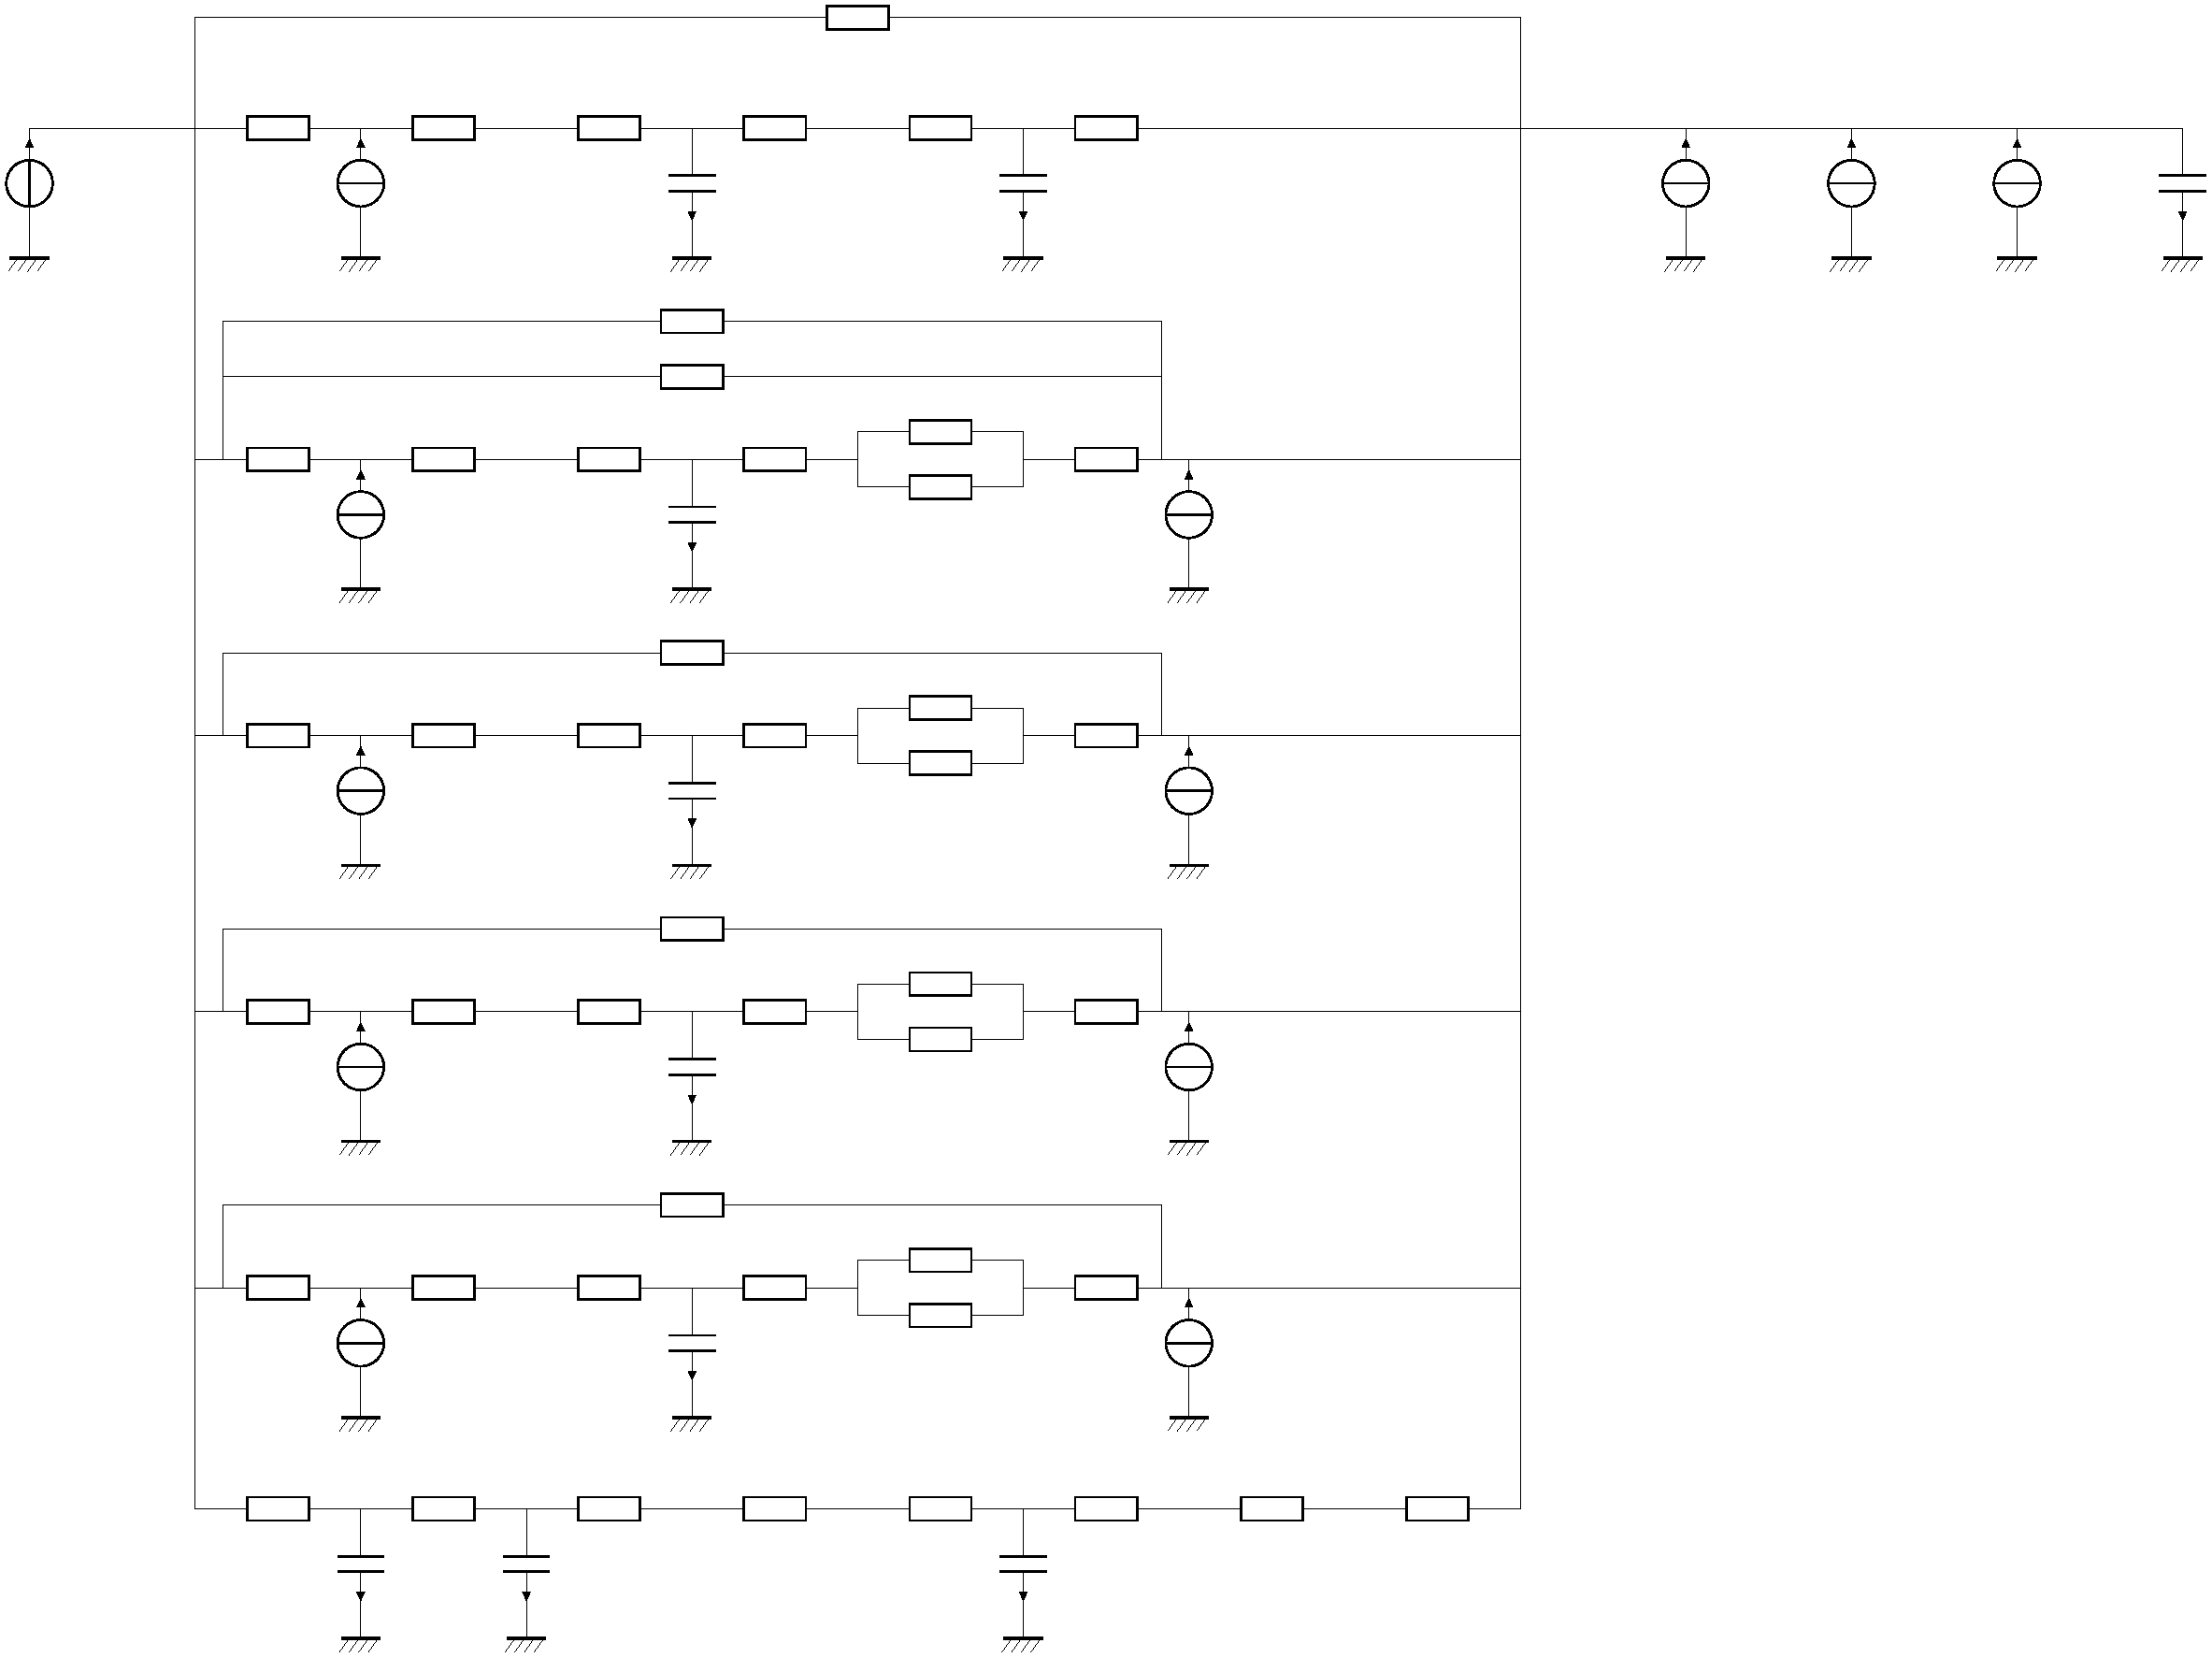
\includegraphics[width=0.99\columnwidth]{figures/RC_genmod_unlabeled.pdf}
            \caption{\label{fig:rc_mod} Diagram of the general RC model.}
            \begin{quote}
                \vspace{-2mm}
                \small\noindent
                Description. il faut ajouter les noms des composants 
              \end{quote}
        \end{figure}  


        Vecteurs $\mathbf{x}$ des températures inertielles ($[10\times 1]$) et vecteur $\mathbf{u}$ des températures et flux variables ($[15\times 1]$)

        \begin{equation}
          \begin{dcases}
            \mathbf{x} = [T_i, T_{w_0}, T_{w_1}, T_{w_2}, T_{w_3}, T_c, T_u, T_f, T_d, T_g]^\top \\
            \mathbf{u} = [T_e, \phi_{sue}, \phi_{sui}, \phi_{sw_0e}, \phi_{sw_0i}, \phi_{sw_1e}, \phi_{sw_1i}, \phi_{sw_2e}, \phi_{sw_2i}, \phi_{sw_3e}, \phi_{sw_3i}, \phi_{hc}, \phi_{i}, \phi_{v\mathrm{meca}}, \phi_{v\mathrm{nat}}]^\top
          \end{dcases}
        \end{equation}

        Matrices de calcul $\mathbb{A}$ ($[10\times 10]$) et $\mathbb{B}$ ($[10\times 15]$)
          % \resizebox{\columnwidth}{!}{
        % \resizebox{\columnwidth}{!}{$
        \begin{equation}\label{eq:rcmatrix}
        \mathbb{A} = 
        \begin{bmatrix}
          a_{00} & a_{01} & a_{02} & a_{03} & a_{04} & a_{05} &        & a_{07} &        &       \\
          a_{10} & a_{11} &        &        &        &        &        &        &        &       \\
          a_{20} &        & a_{22} &        &        &        &        &        &        &       \\
          a_{30} &        &        & a_{33} &        &        &        &        &        &       \\
          a_{40} &        &        &        & a_{44} &        &        &        &        &       \\
          a_{50} &        &        &        &        & a_{55} & a_{56} &        &        &       \\
                 &        &        &        &        & a_{65} & a_{66} &        &        &       \\
          a_{70} &        &        &        &        &        &        & a_{77} & a_{78} & a_{79}\\
                 &        &        &        &        &        &        & a_{87} & a_{88} & a_{89}\\
                 &        &        &        &        &        &        & a_{97} & a_{98} & a_{99}\\
        \end{bmatrix}
        \end{equation}


        \begin{equation}
          \mathbb{B} = \begin{bmatrix}
  b_{00} &        & b_{02} &        & b_{04} &        & b_{06} &        & b_{08} &        & b_{010}& b_{011}& b_{012}& b_{013}& b_{014}\\
  b_{10} &        &        & b_{13} &        &        &        &        &        &        &        &        &        &        &       \\
  b_{20} &        &        &        &        & b_{25} &        &        &        &        &        &        &        &        &       \\
  b_{30} &        &        &        &        &        &        & b_{37} &        &        &        &        &        &        &       \\
  b_{40} &        &        &        &        &        &        &        &        & b_{49} &        &        &        &        &       \\
  b_{50} & b_{51} &        &        &        &        &        &        &        &        &        &        &        &        &       \\
  b_{60} & b_{61} &        &        &        &        &        &        &        &        &        &        &        &        &       \\
         &        &        &        &        &        &        &        &        &        &        &        &        &        &       \\
         &        &        &        &        &        &        &        &        &        &        &        &        &        &       \\
  b_{90} &        &        &        &        &        &        &        &        &        &        &        &        &        &       \\
\end{bmatrix}
        \end{equation}


        % paragraph general_rc_model (end)

            \paragraph{Internal solar gains}\mbox{}\\ % (fold)
            \label{par:internal_solar_gains}

            ajouter un schéma pour chacun des deux facteurs (\ref{fig:solar_mask_diagram})

                \begin{figure}[ht]
                \centering
                
                
\includegraphics[width=0.32\columnwidth]{figures/solar_factor_direct.png}
                
\includegraphics[width=0.32\columnwidth]{figures/solar_factor_diffuse.png}
                
                \caption{\label{fig:solar_mask_diagram} Diagram of solar masks.}
                    \begin{quote}
                        \vspace{-2mm}
                        \small\noindent
                        \textbf{(left to right)} Description.
                    \end{quote}
                \end{figure}  


                \begin{subequations}
                    \begin{empheq}[left=\empheqlbrace]{align}
                        f_{\mathrm{direct}} &= 1-\frac{d \times \tan(\alpha) - e_c}{h_w} \label{eq:solar_factor_direct}\\
                        f_{\mathrm{diffuse}} &= 1-\frac{1}{\pi/2}~\tan^{-1}\left(\frac{d}{e_c + h_w/2}\right)\label{eq:solar_factor_diffuse}
                    \end{empheq}
                \end{subequations}

                (\ref{fig:solar_mask})

                \begin{figure}[ht]
                \centering
                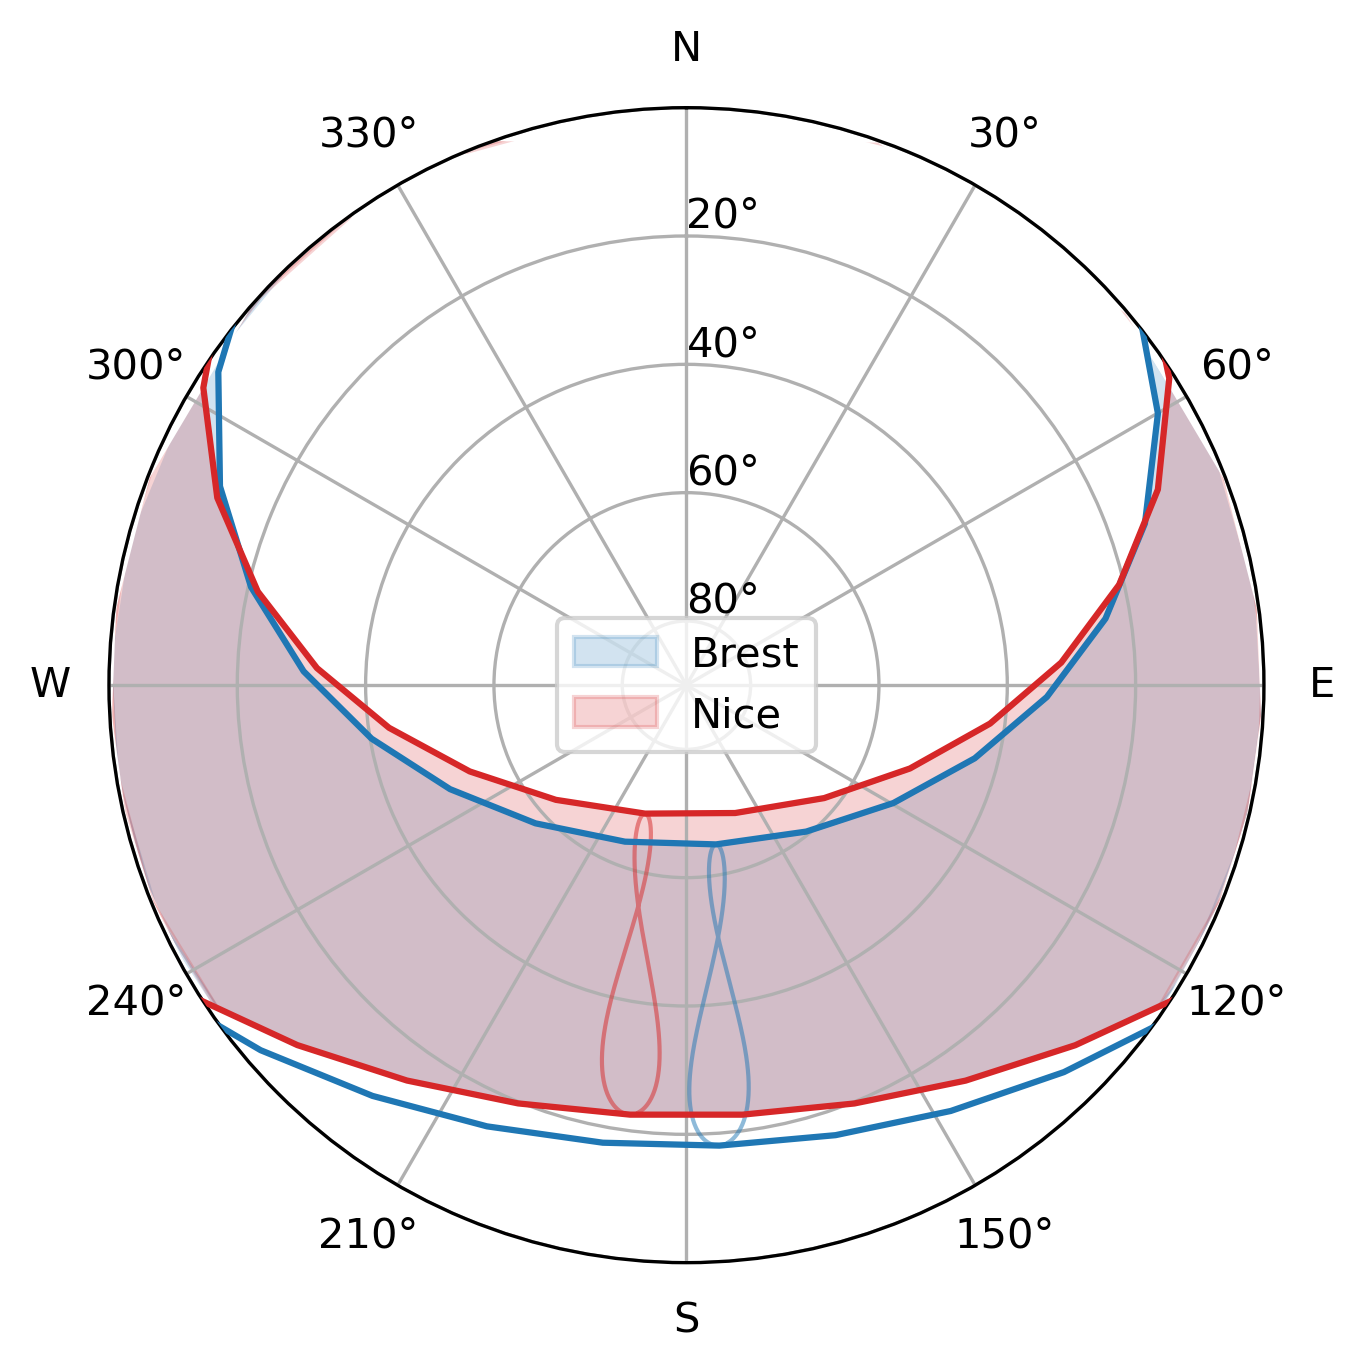
\includegraphics[width=0.32\columnwidth]{figures/sun_path_Brest_Nice_2022.png}
                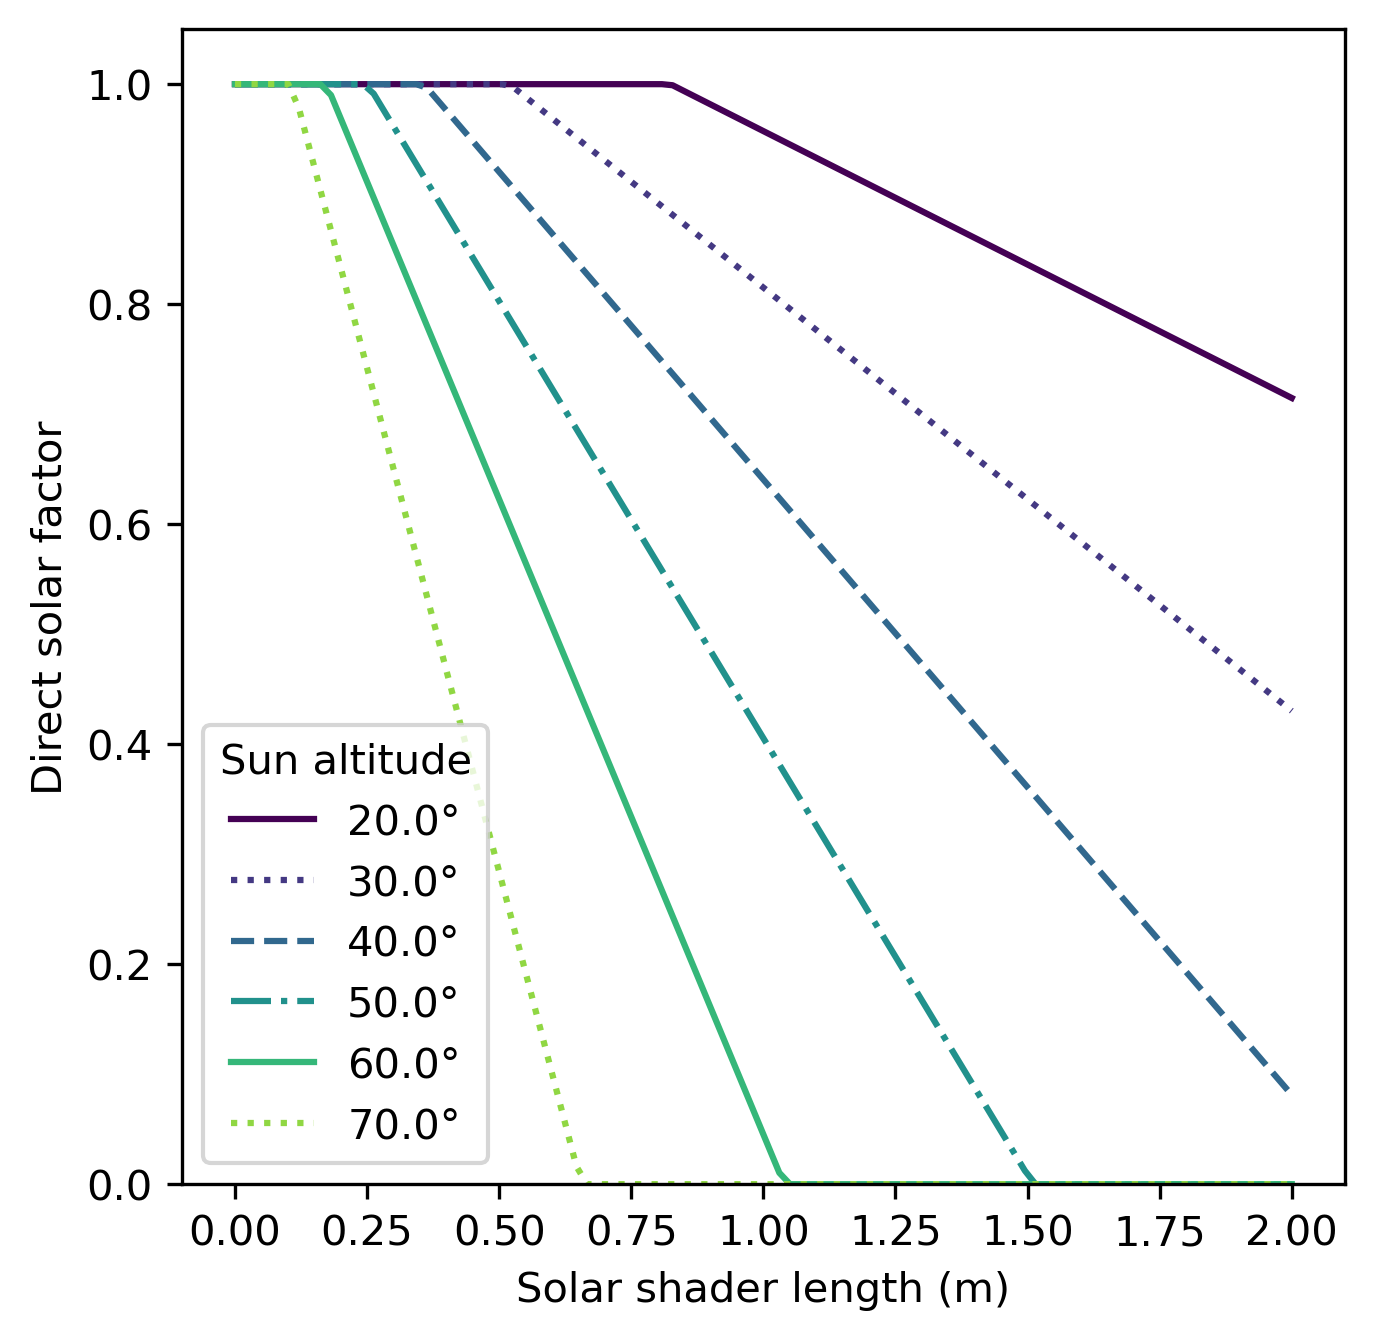
\includegraphics[width=0.32\columnwidth]{figures/direct_solar_factor_masking.png}
                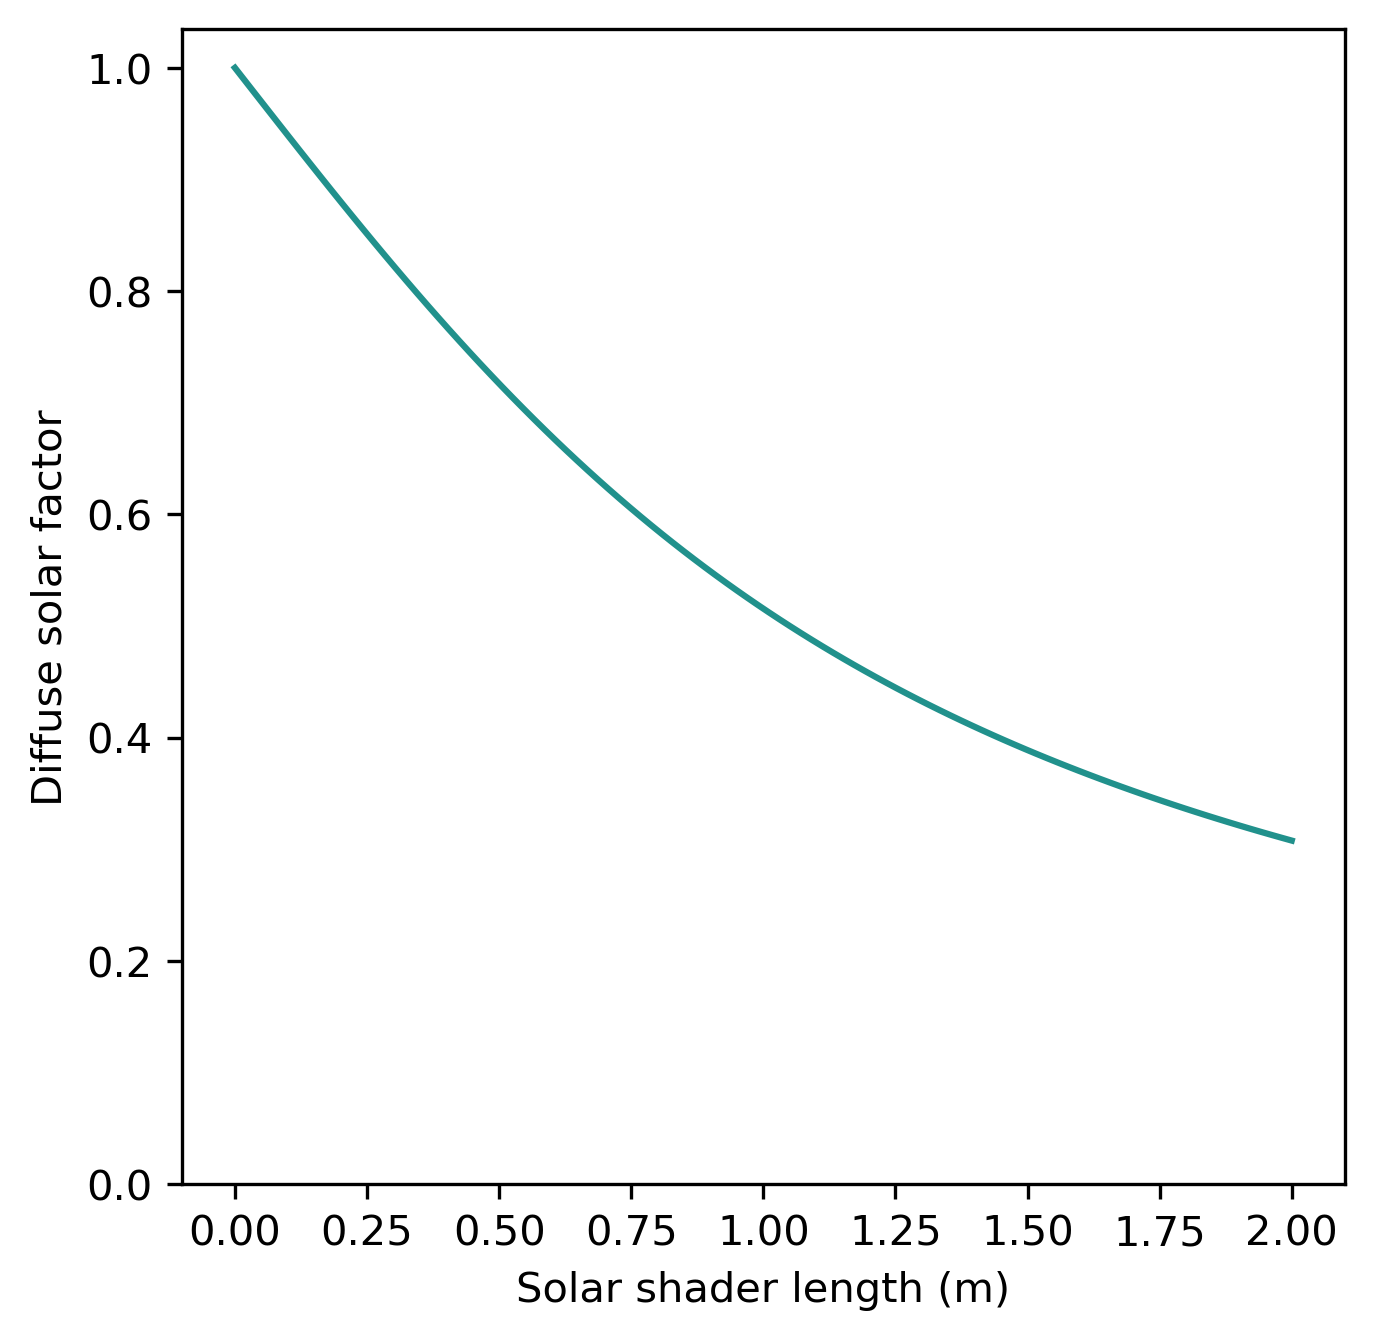
\includegraphics[width=0.32\columnwidth]{figures/diffuse_solar_factor_masking.png}
                \caption{\label{fig:solar_mask} Solar path graph and effects of solar protection length on solar transmission factor.}
                    \begin{quote}
                        \vspace{-2mm}
                        \small\noindent
                        \textbf{(left to right)} Description. \eqref{eq:solar_factor_direct}, \eqref{eq:solar_factor_diffuse}
                    \end{quote}
                \end{figure}  
            
            % paragraph internal_solar_gains (end)
        
        % subsubsection model_construction (end)

        \subsubsection{Model computation} % (fold)
        \label{ssub:model_computation}
        
        mathematiques derriere le calcul
        \cite{madsen_estimation_1995}, \cite{rouchier_solving_2018}

        
        % subsubsection model_computation (end)

        \subsubsection{Model verification} % (fold)
        \label{ssub:model_verification}
        
        resultats de comparaisons avec TABULA (\ref{fig:tabula_verif})

        parler des hypothèses propres à la méthodologie de \textcite{pouget_consultants_batiments_2015} et des modifications de behaviour par rapport au conventionnel. 

        \begin{figure}[ht]
            \centering
            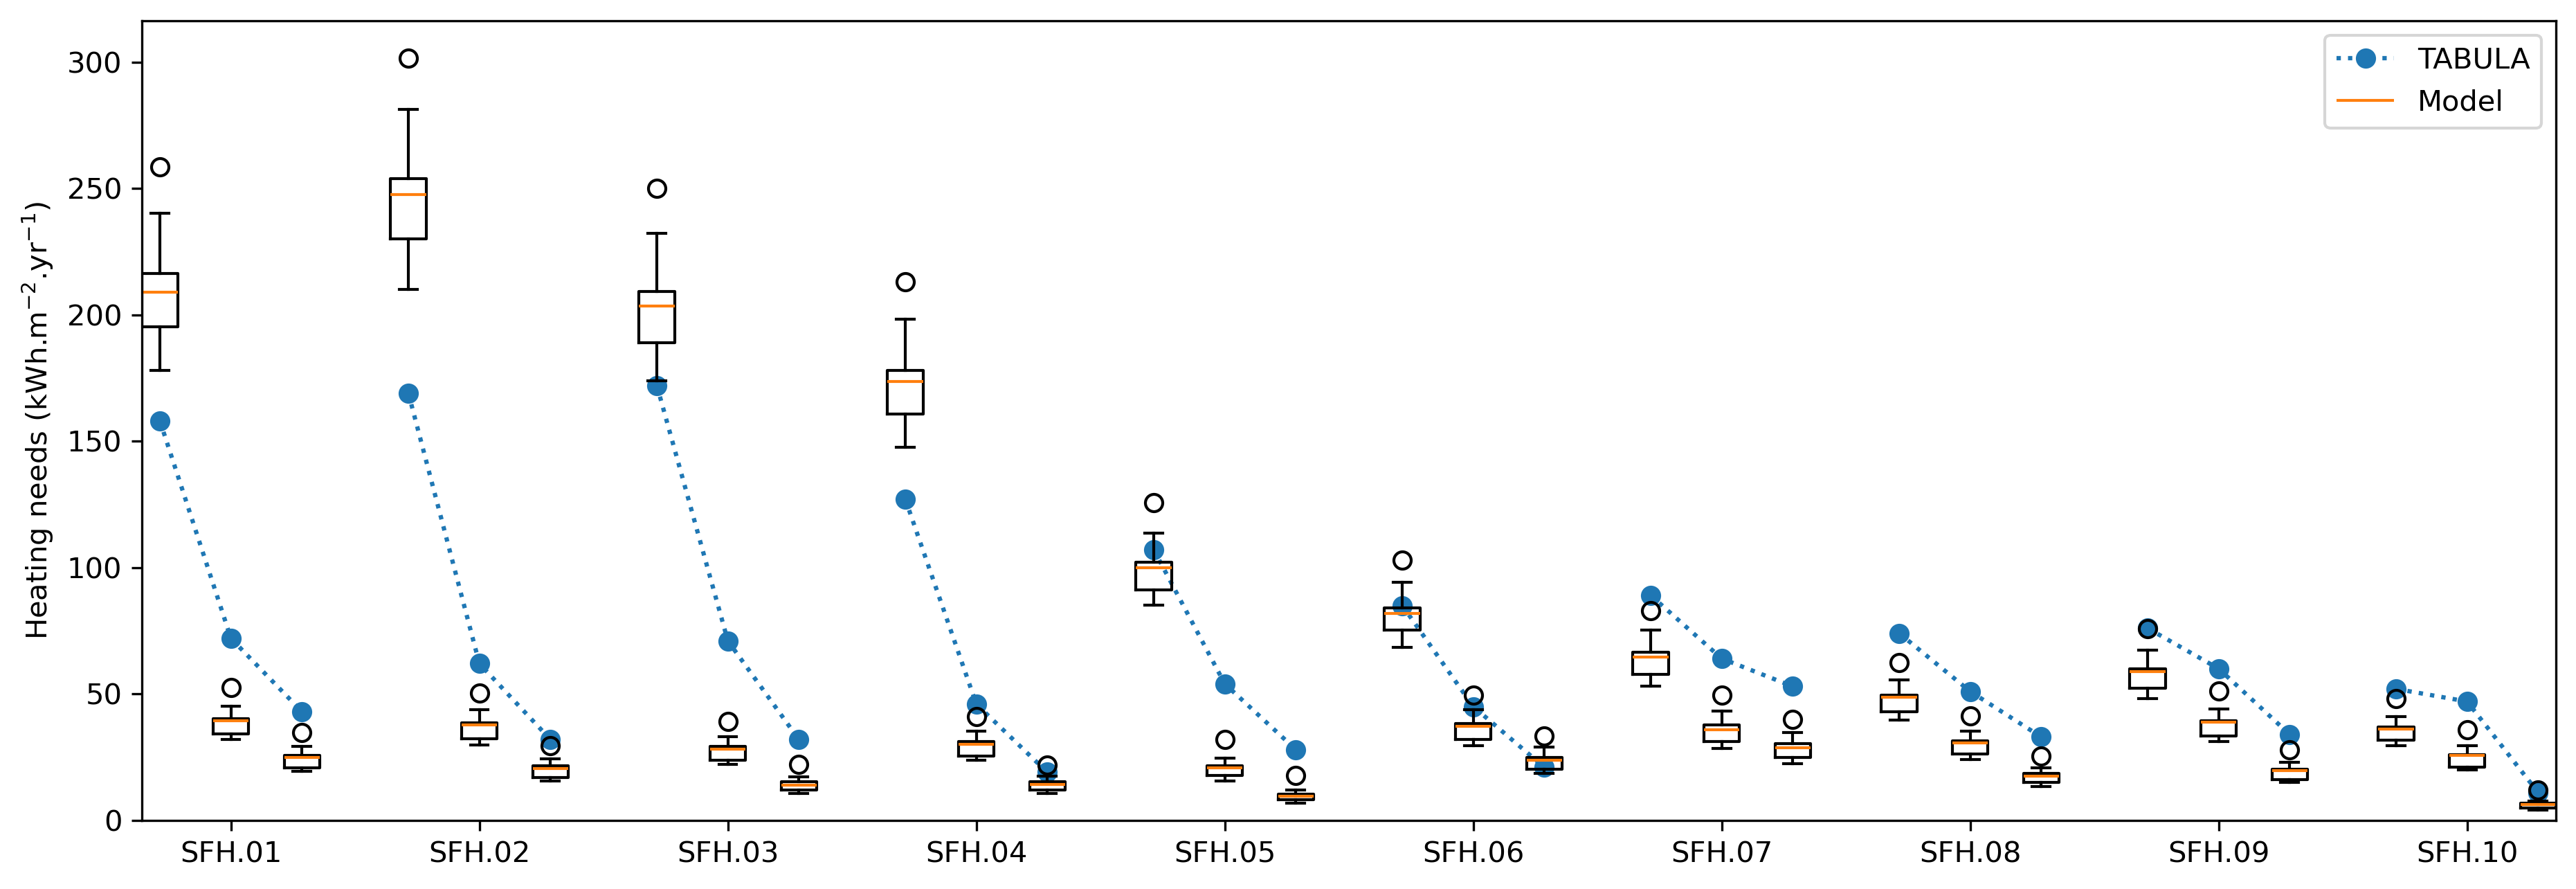
\includegraphics[width=0.99\columnwidth]{figures/SFH_TABULA_consumption.png}
            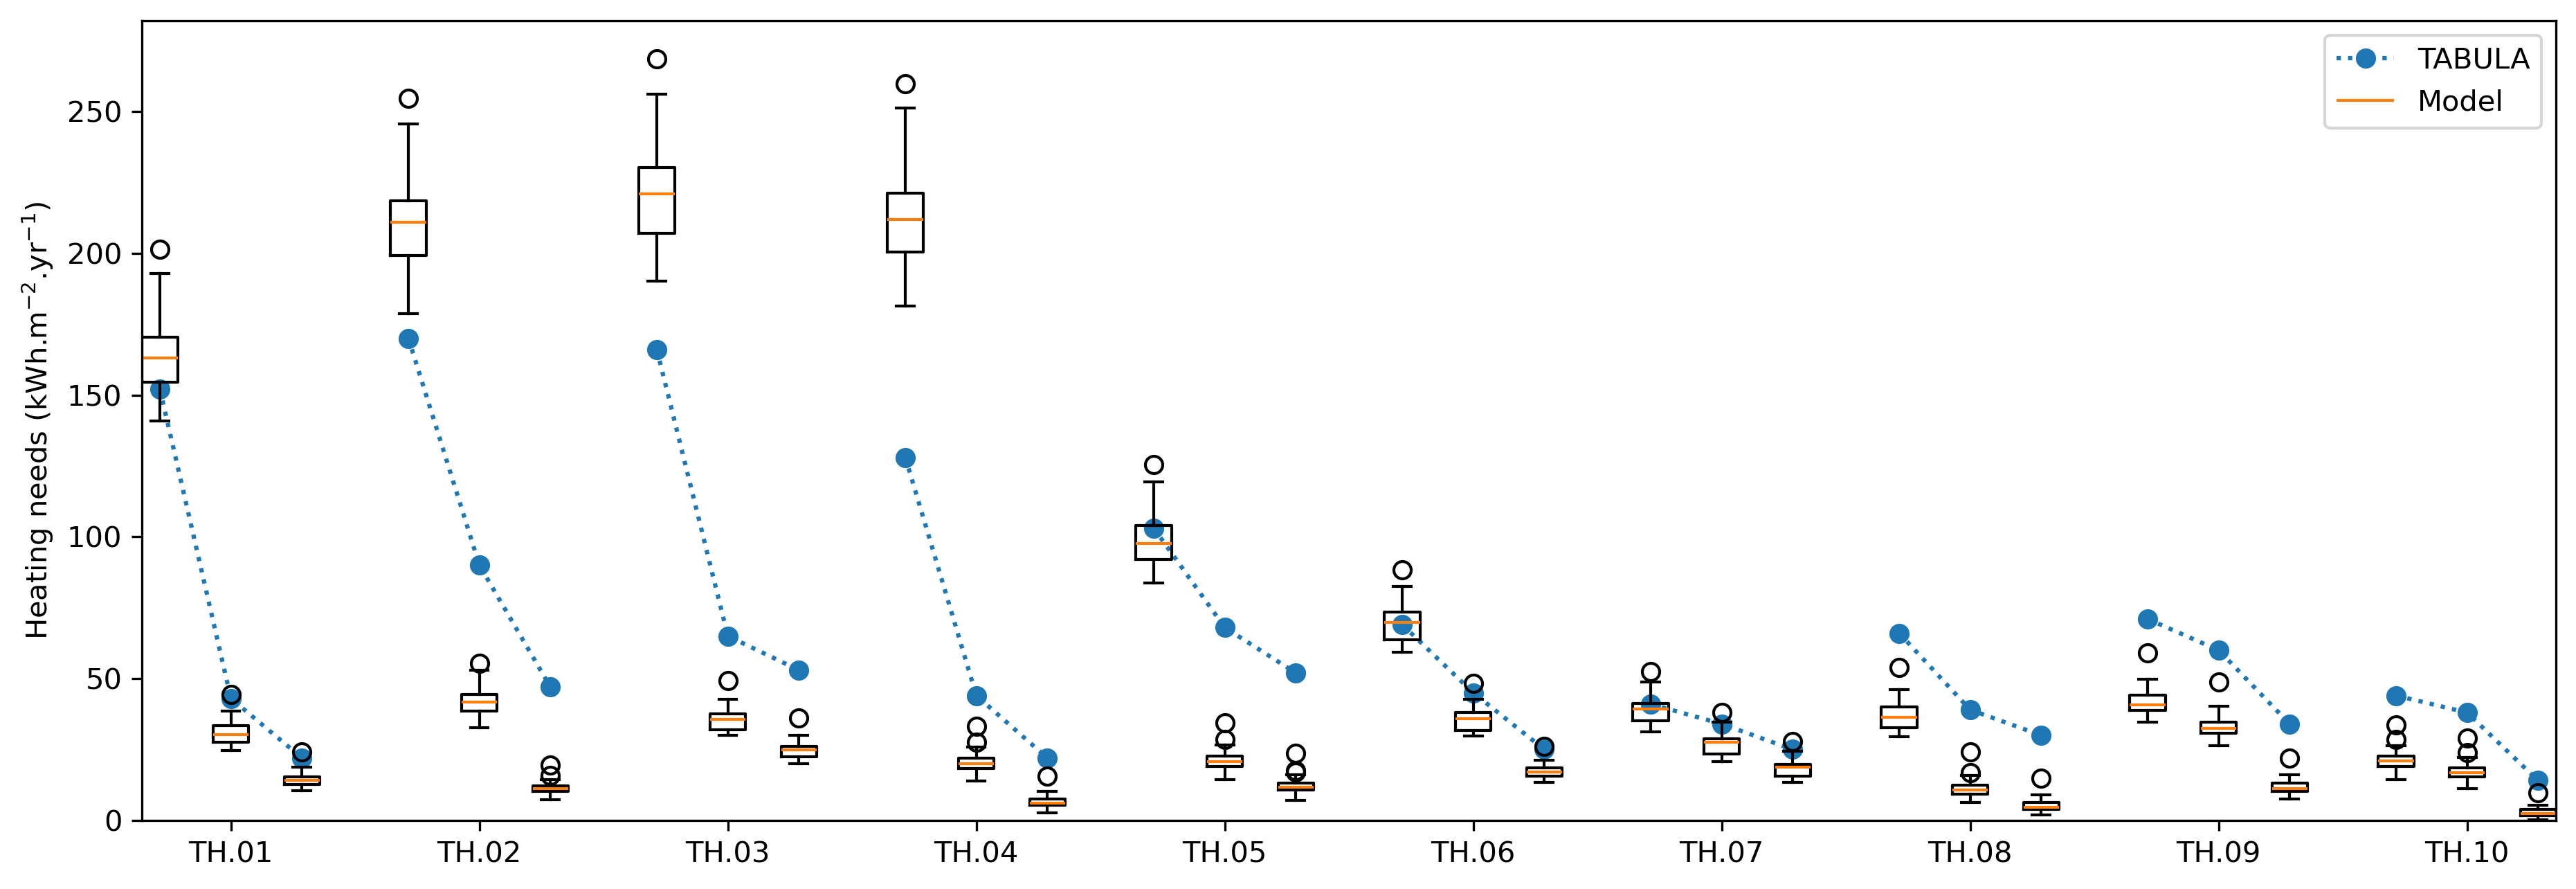
\includegraphics[width=0.99\columnwidth]{figures/TH_TABULA_consumption.png}
            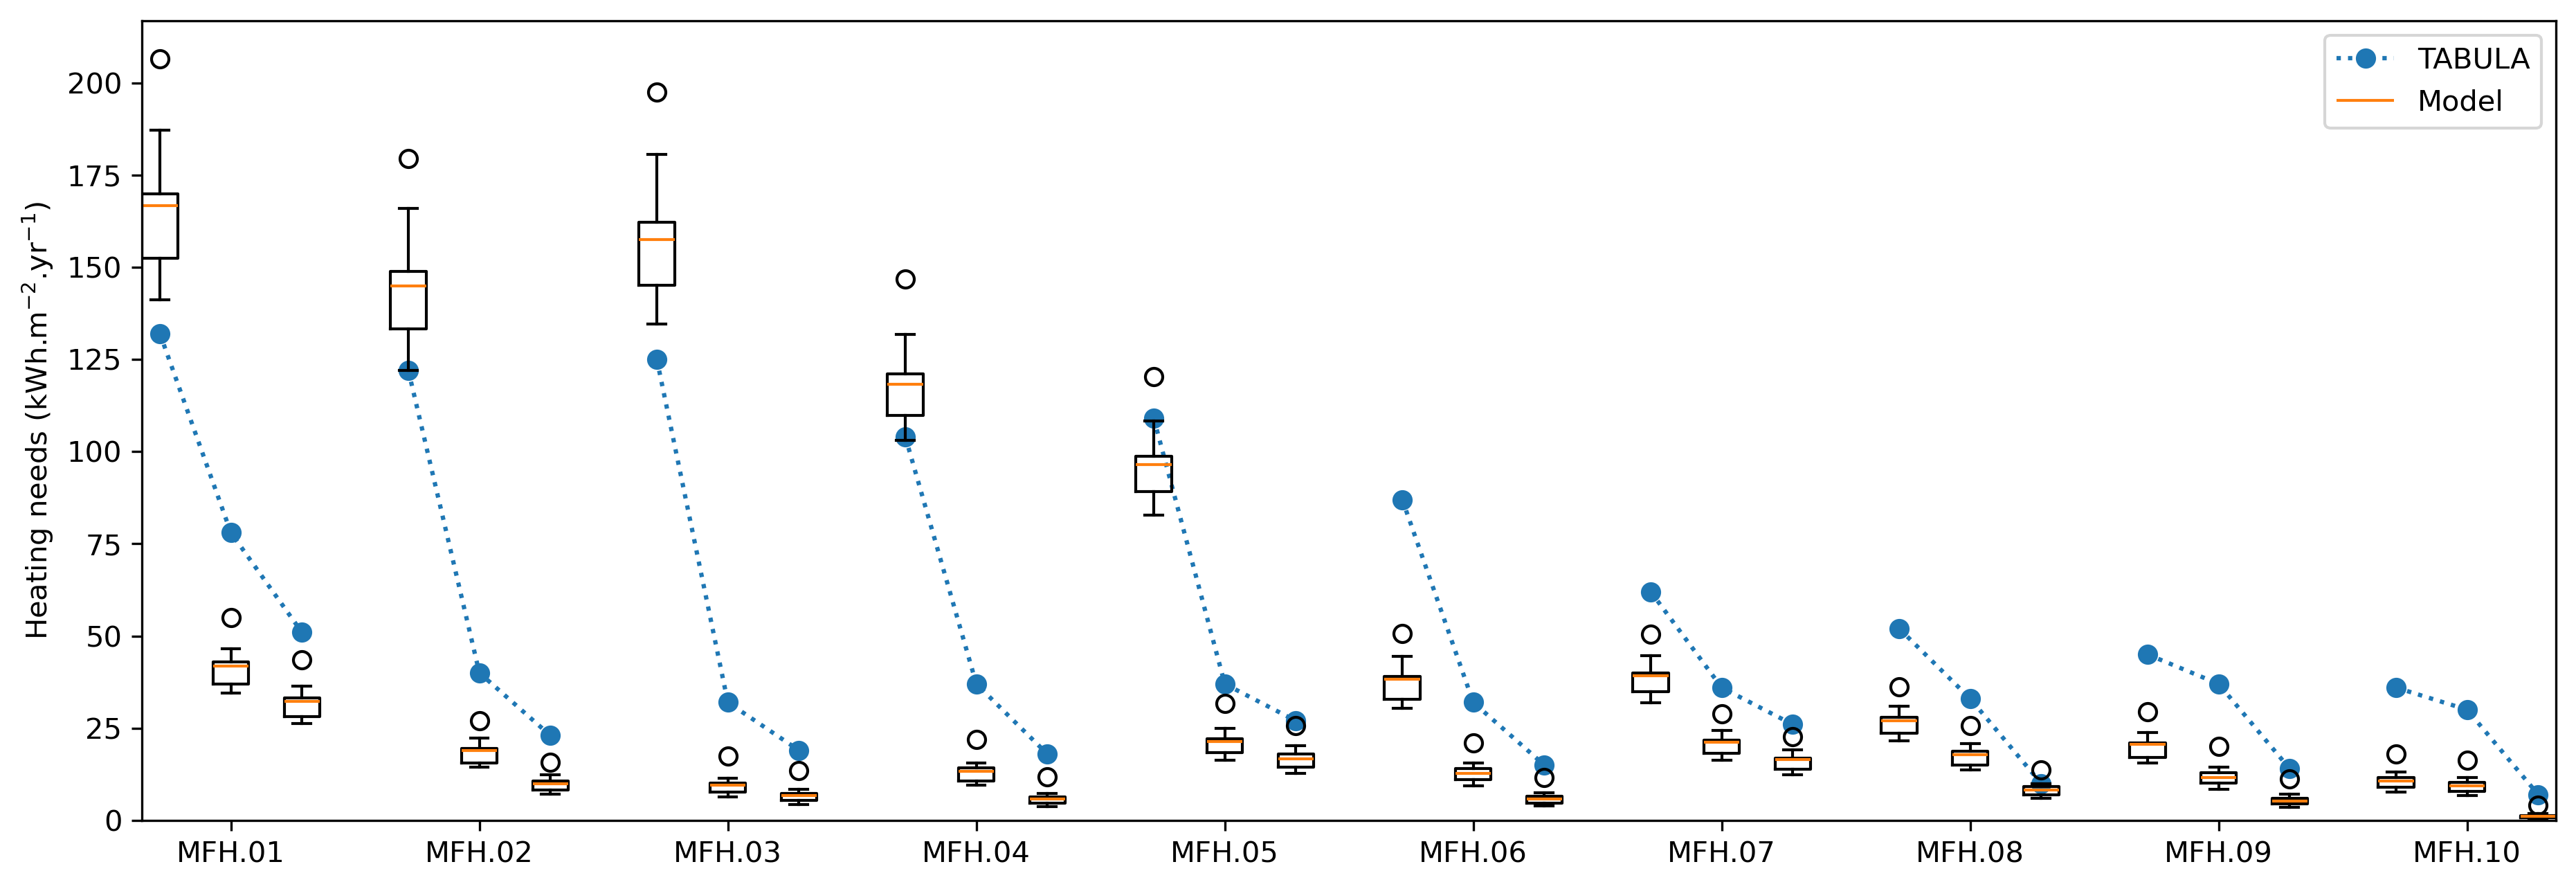
\includegraphics[width=0.99\columnwidth]{figures/MFH_TABULA_consumption.png}
            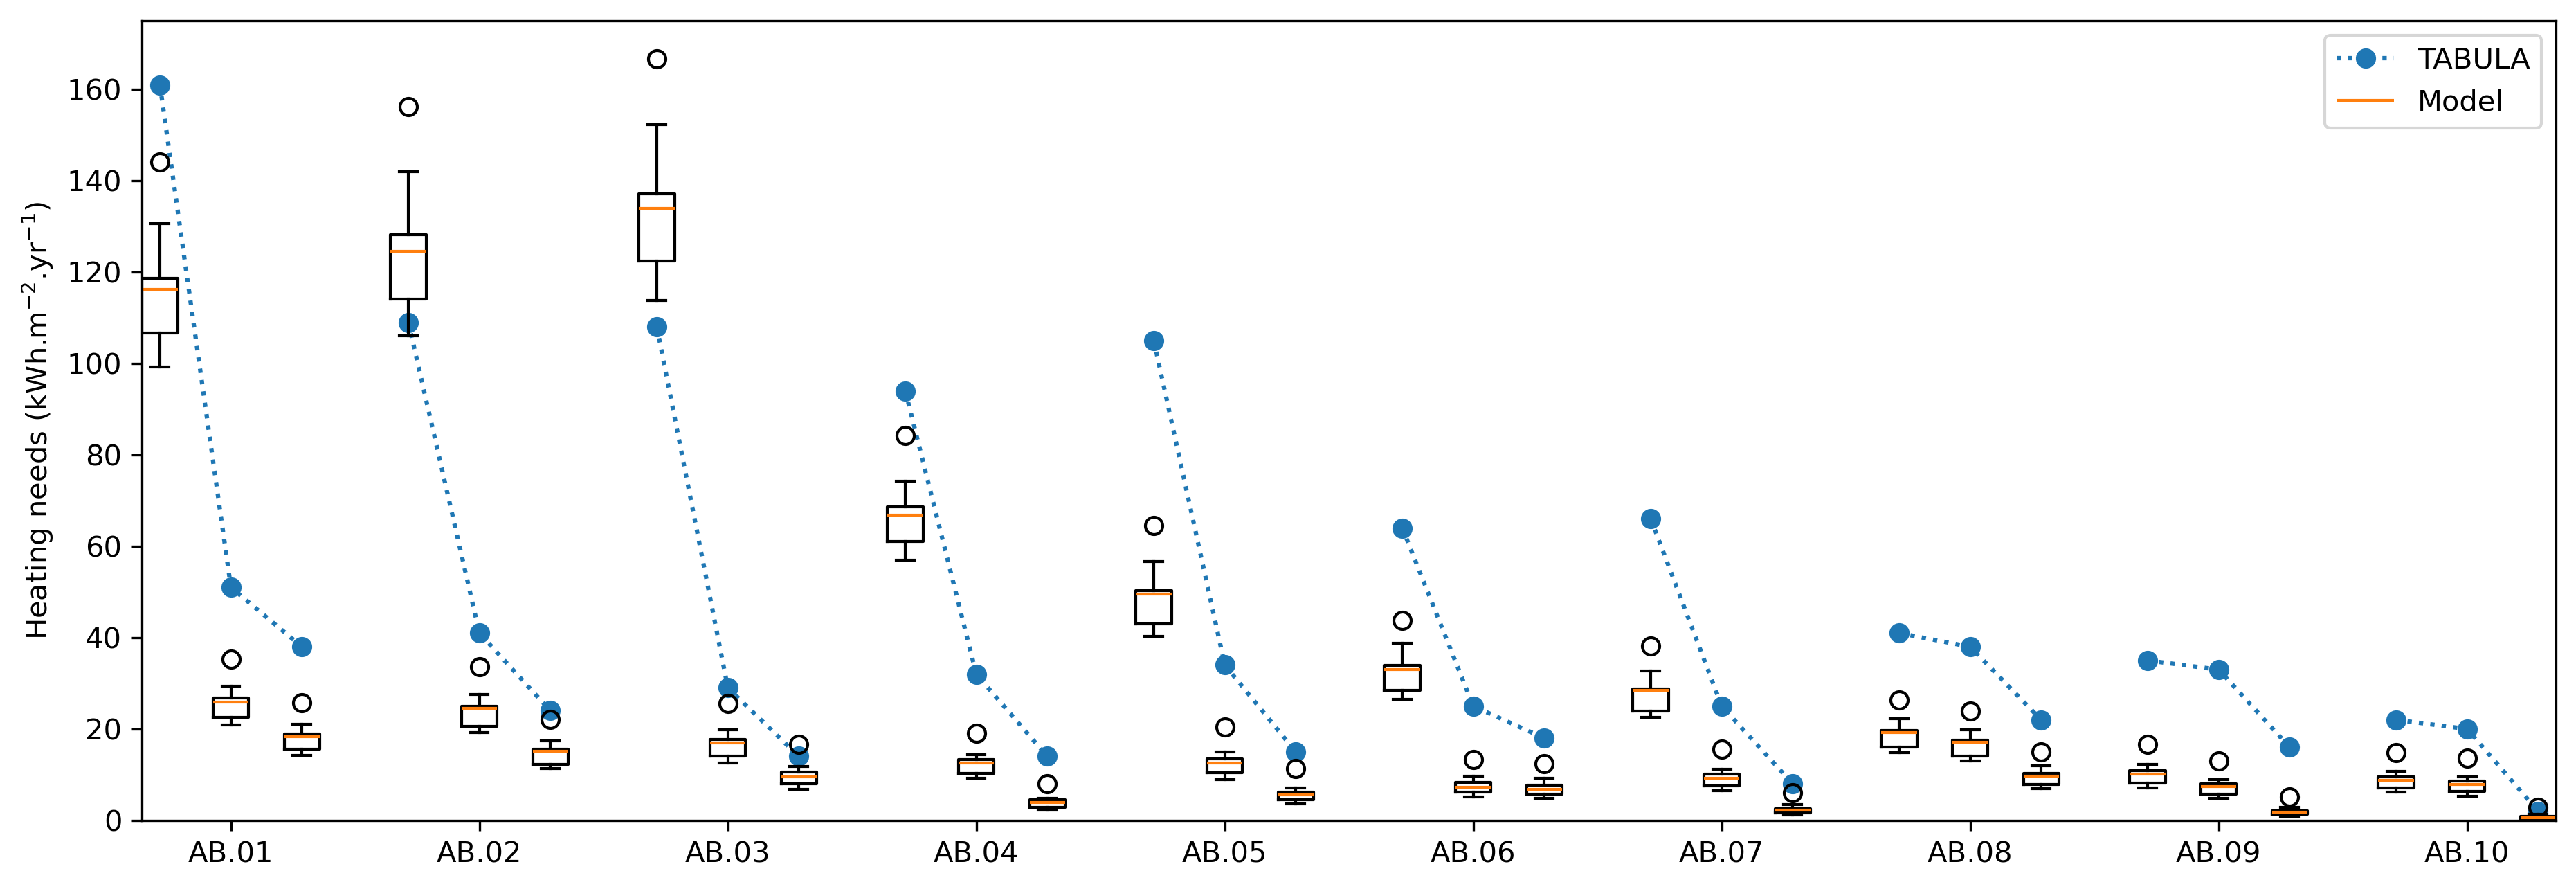
\includegraphics[width=0.99\columnwidth]{figures/AB_TABULA_consumption.png}
            \caption{\label{fig:tabula_verif} Heating needs comparison with TABULA data.}
                \begin{quote}
                    \vspace{-2mm}
                    \small\noindent
                    \textbf{(top to bottom)} Description. 
                \end{quote}
        \end{figure}  

        comparaison avec \textcite{pomianowski_method_2023} (en faire d'autres)
        % subsubsection model_verification (end)

    % subsection rc_analogy_and_computation (end)

    \subsection{TABULA typologies} % (fold)
    \label{sub:tabula_typologies}
    
        \subsubsection{Typologies definition} % (fold)
        \label{ssub:typologies_definition}
        
        historique et description
        \cite{pouget_consultants_batiments_2015}, \cite{loga_tabula_2016}

        valeurs moyennes d'interet pour les typologies et les 3 niveaux (tableau)

        typologies non isolées en état initial 
        % subsubsection typologies_definition (end)

        \subsubsection{Typology representation in the French building stock} % (fold)
        \label{ssub:typologies_distribution}
        
        representativite des typologies dans le parc français (\ref{fig:tab_stock})

        \begin{figure}[ht]
            \centering
            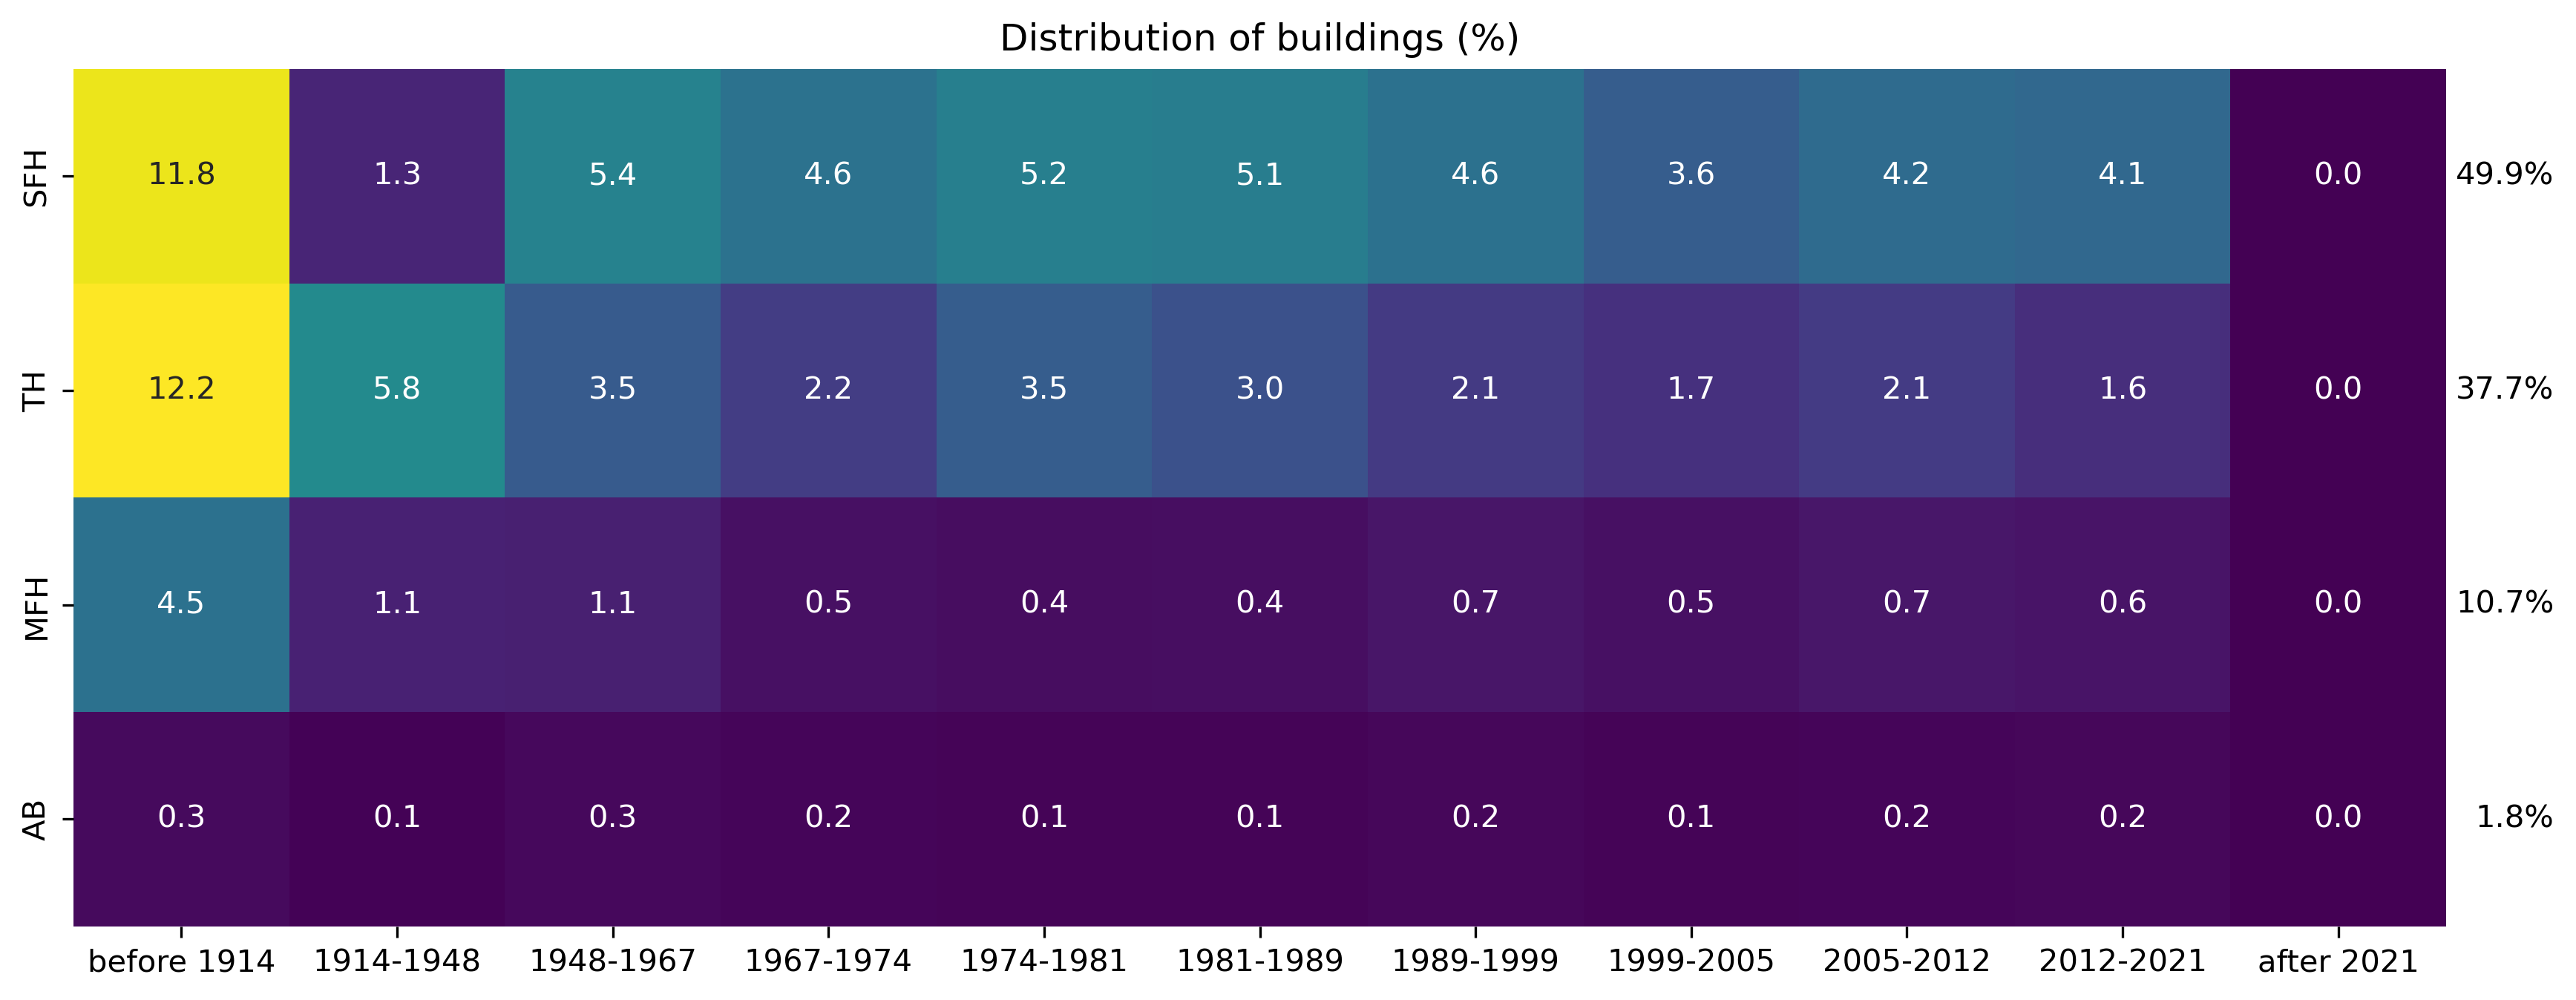
\includegraphics[width=0.99\columnwidth]{figures/bgc_distribution_tabula_buildings_ponderated.png}\\
            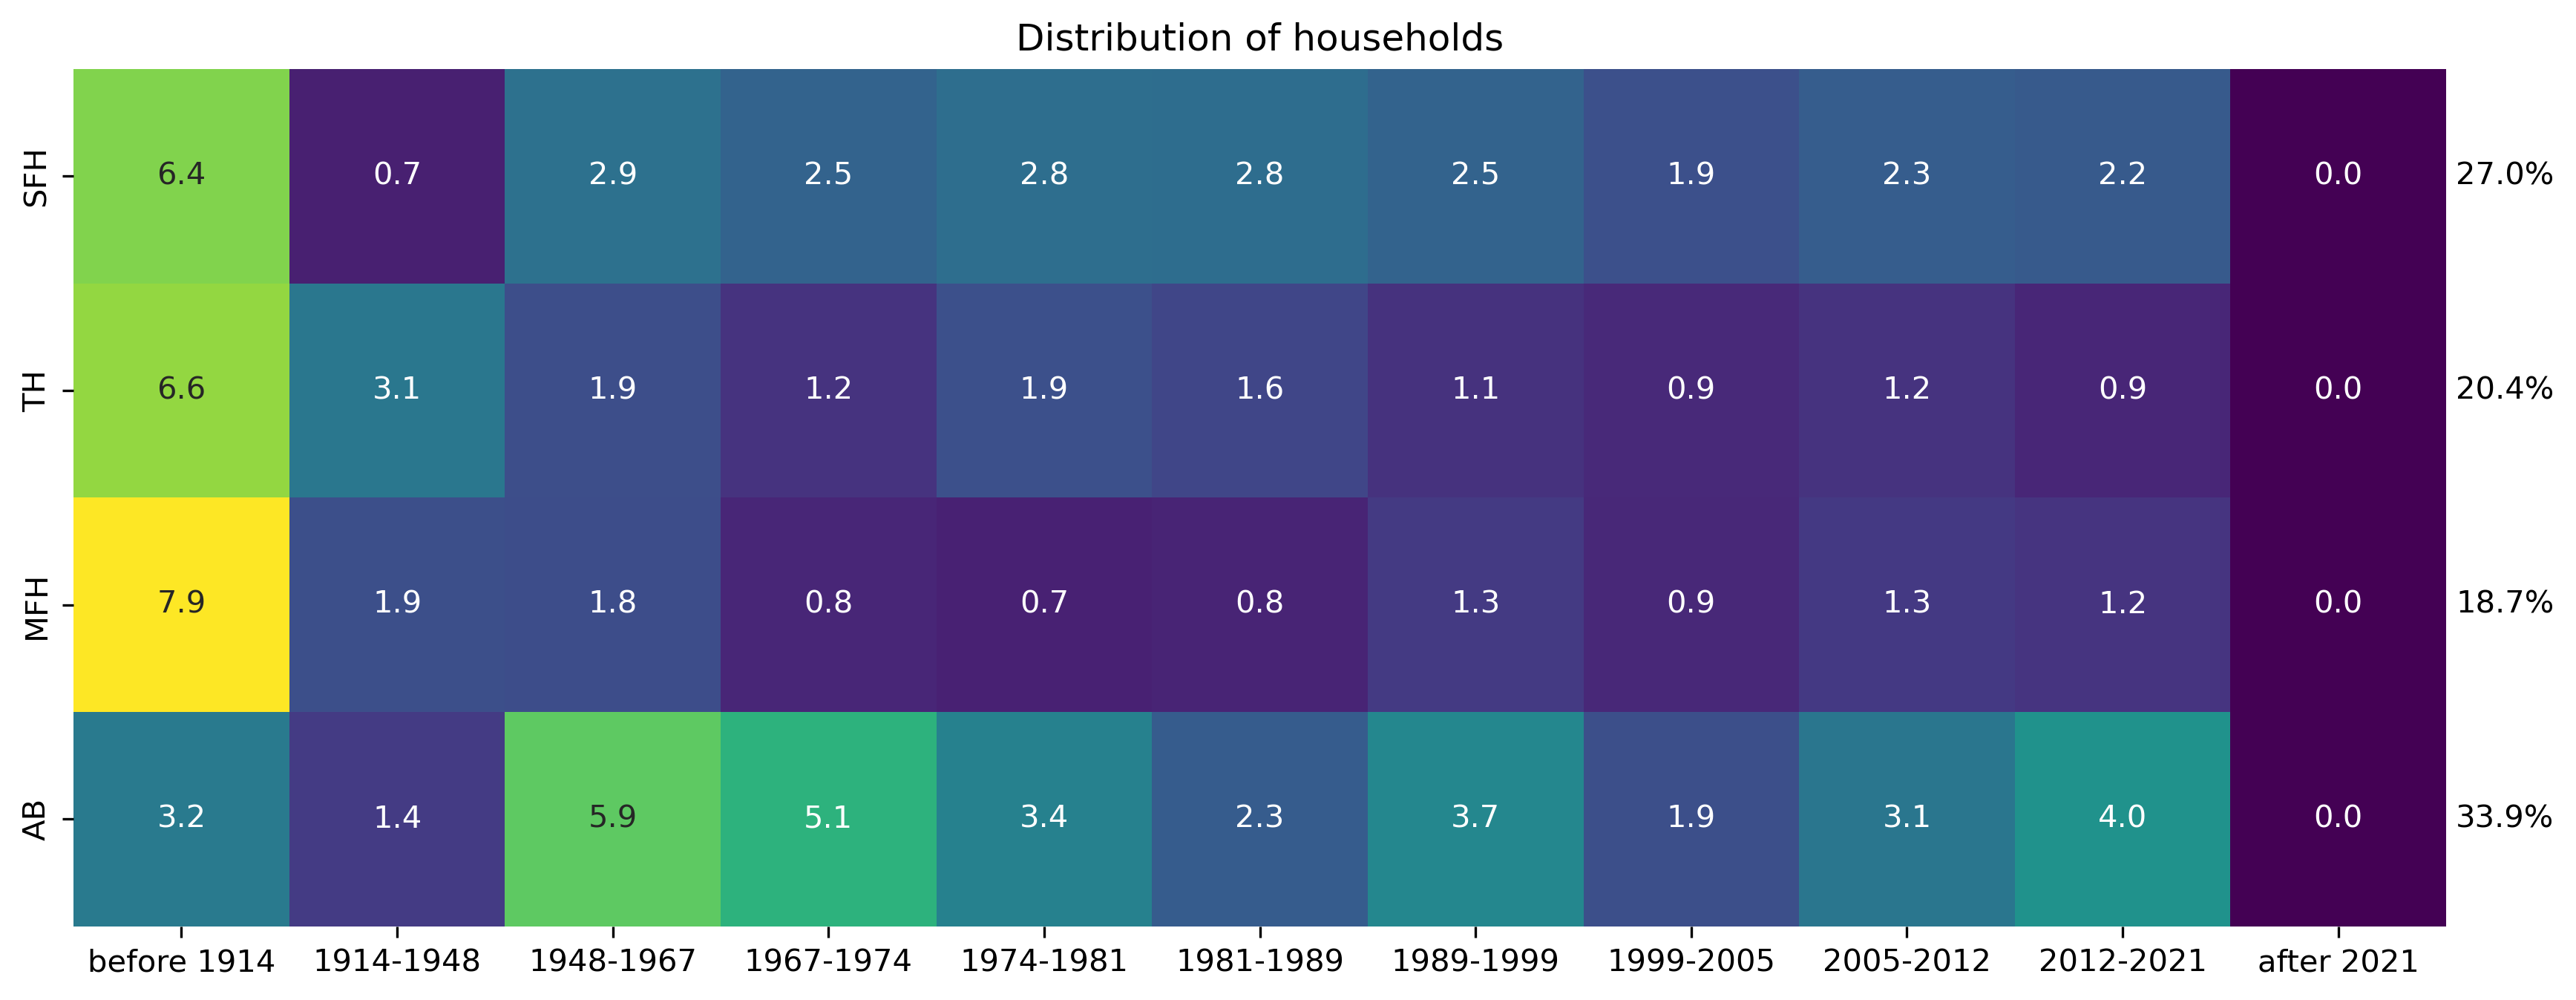
\includegraphics[width=0.99\columnwidth]{figures/bgc_distribution_tabula_households_ponderated.png}
            \caption{\label{fig:tab_stock} Distribution of TABULA typologies in the French building stock.}
            \begin{quote}
                \vspace{-2mm}
                \small\noindent
                \textbf{(top to bottom)} Description.  
              \end{quote}
        \end{figure}

        detail de la methode pour la séparation entre SFH et TH

        




        % subsubsection typologies_distribution (end)


    

    % subsection tabula_typologies (end)

    \subsection{Weather data} % (fold)
    \label{sub:weather_data}

        \subsubsection{French climate zones} % (fold)
        \label{ssub:french_climate_zones}

        utilisation des zones climatiques françaises : limiter les calculs, la complexite, mais aussi s'inscrire dans les politiuqes de renovations qui les utilisent (CEE (\cite{ademe_french_2011}), MPR (\cite{anah_aides_2024}))

        definitions des prefecture centrales (\ref{fig:zcl})
        \begin{equation}
            \label{eq:pref_centr}
            p_c = \min_{d \in \mathbf{d}_c} \left(\|\mathbf{c}_c - \mathbf{c}_{dp}\|_2 \right)
        \end{equation}
        With,
        $$
        \begin{dcases}
            \mathbf{d}_c&\text{: list of departments $d$ in climate zone $c$}\\
            \mathbf{c}_c&\text{: geographic coordinates of climate zone $c$ centroid}\\
            \mathbf{c}_{dp}&\text{: geographic coordinates of department $d$ prefecture}\\
        \end{dcases}
        $$

        \begin{figure}[ht]
            \centering
            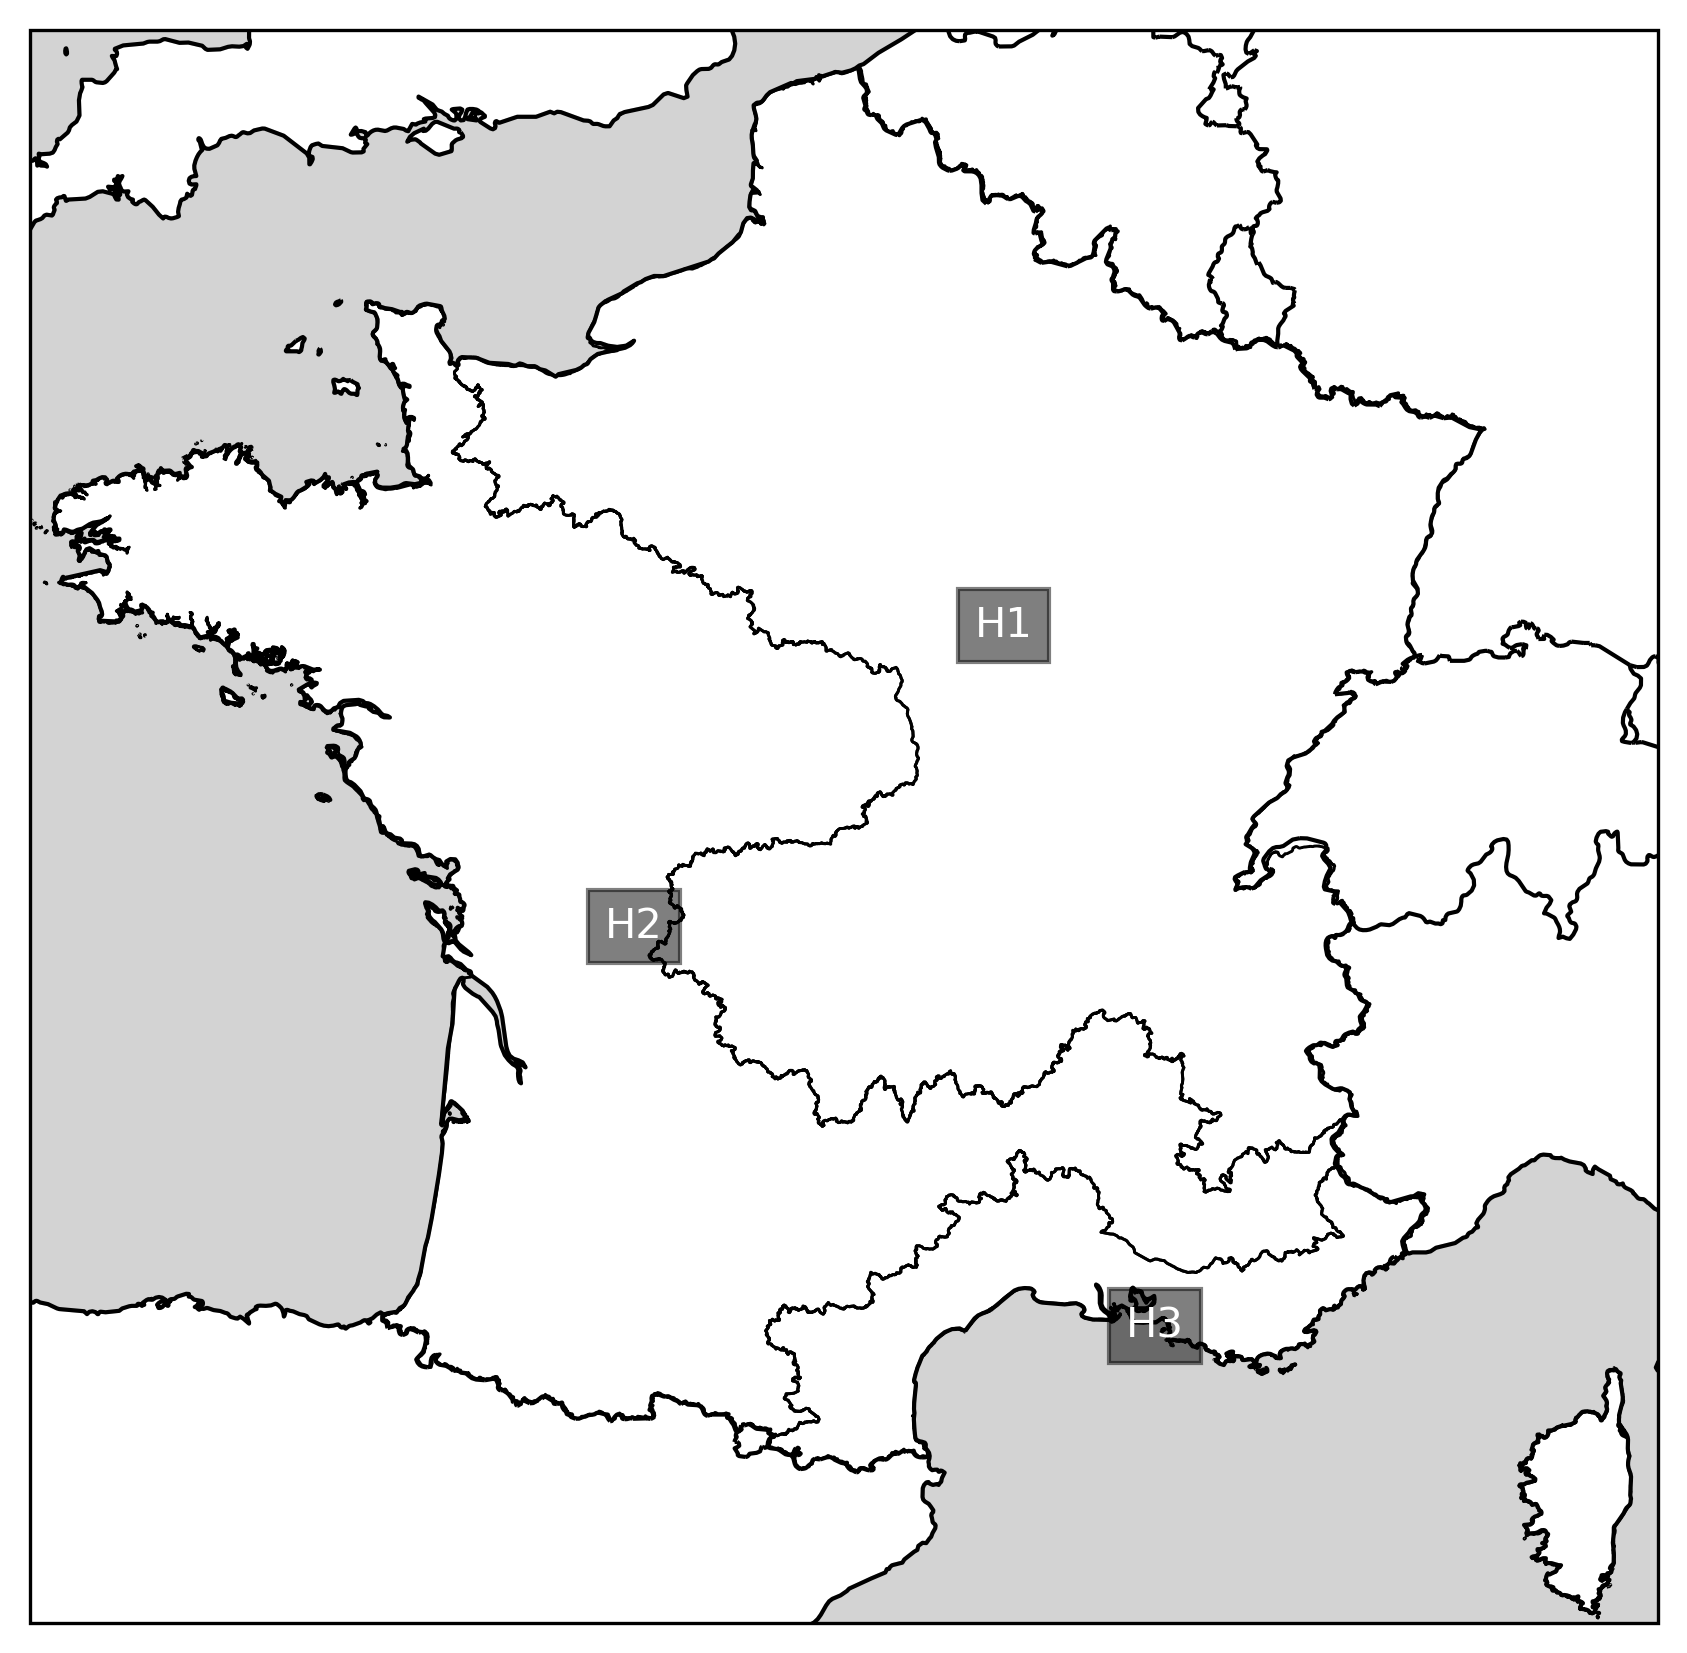
\includegraphics[width=0.32\columnwidth]{figures/zcl_winter.png}
            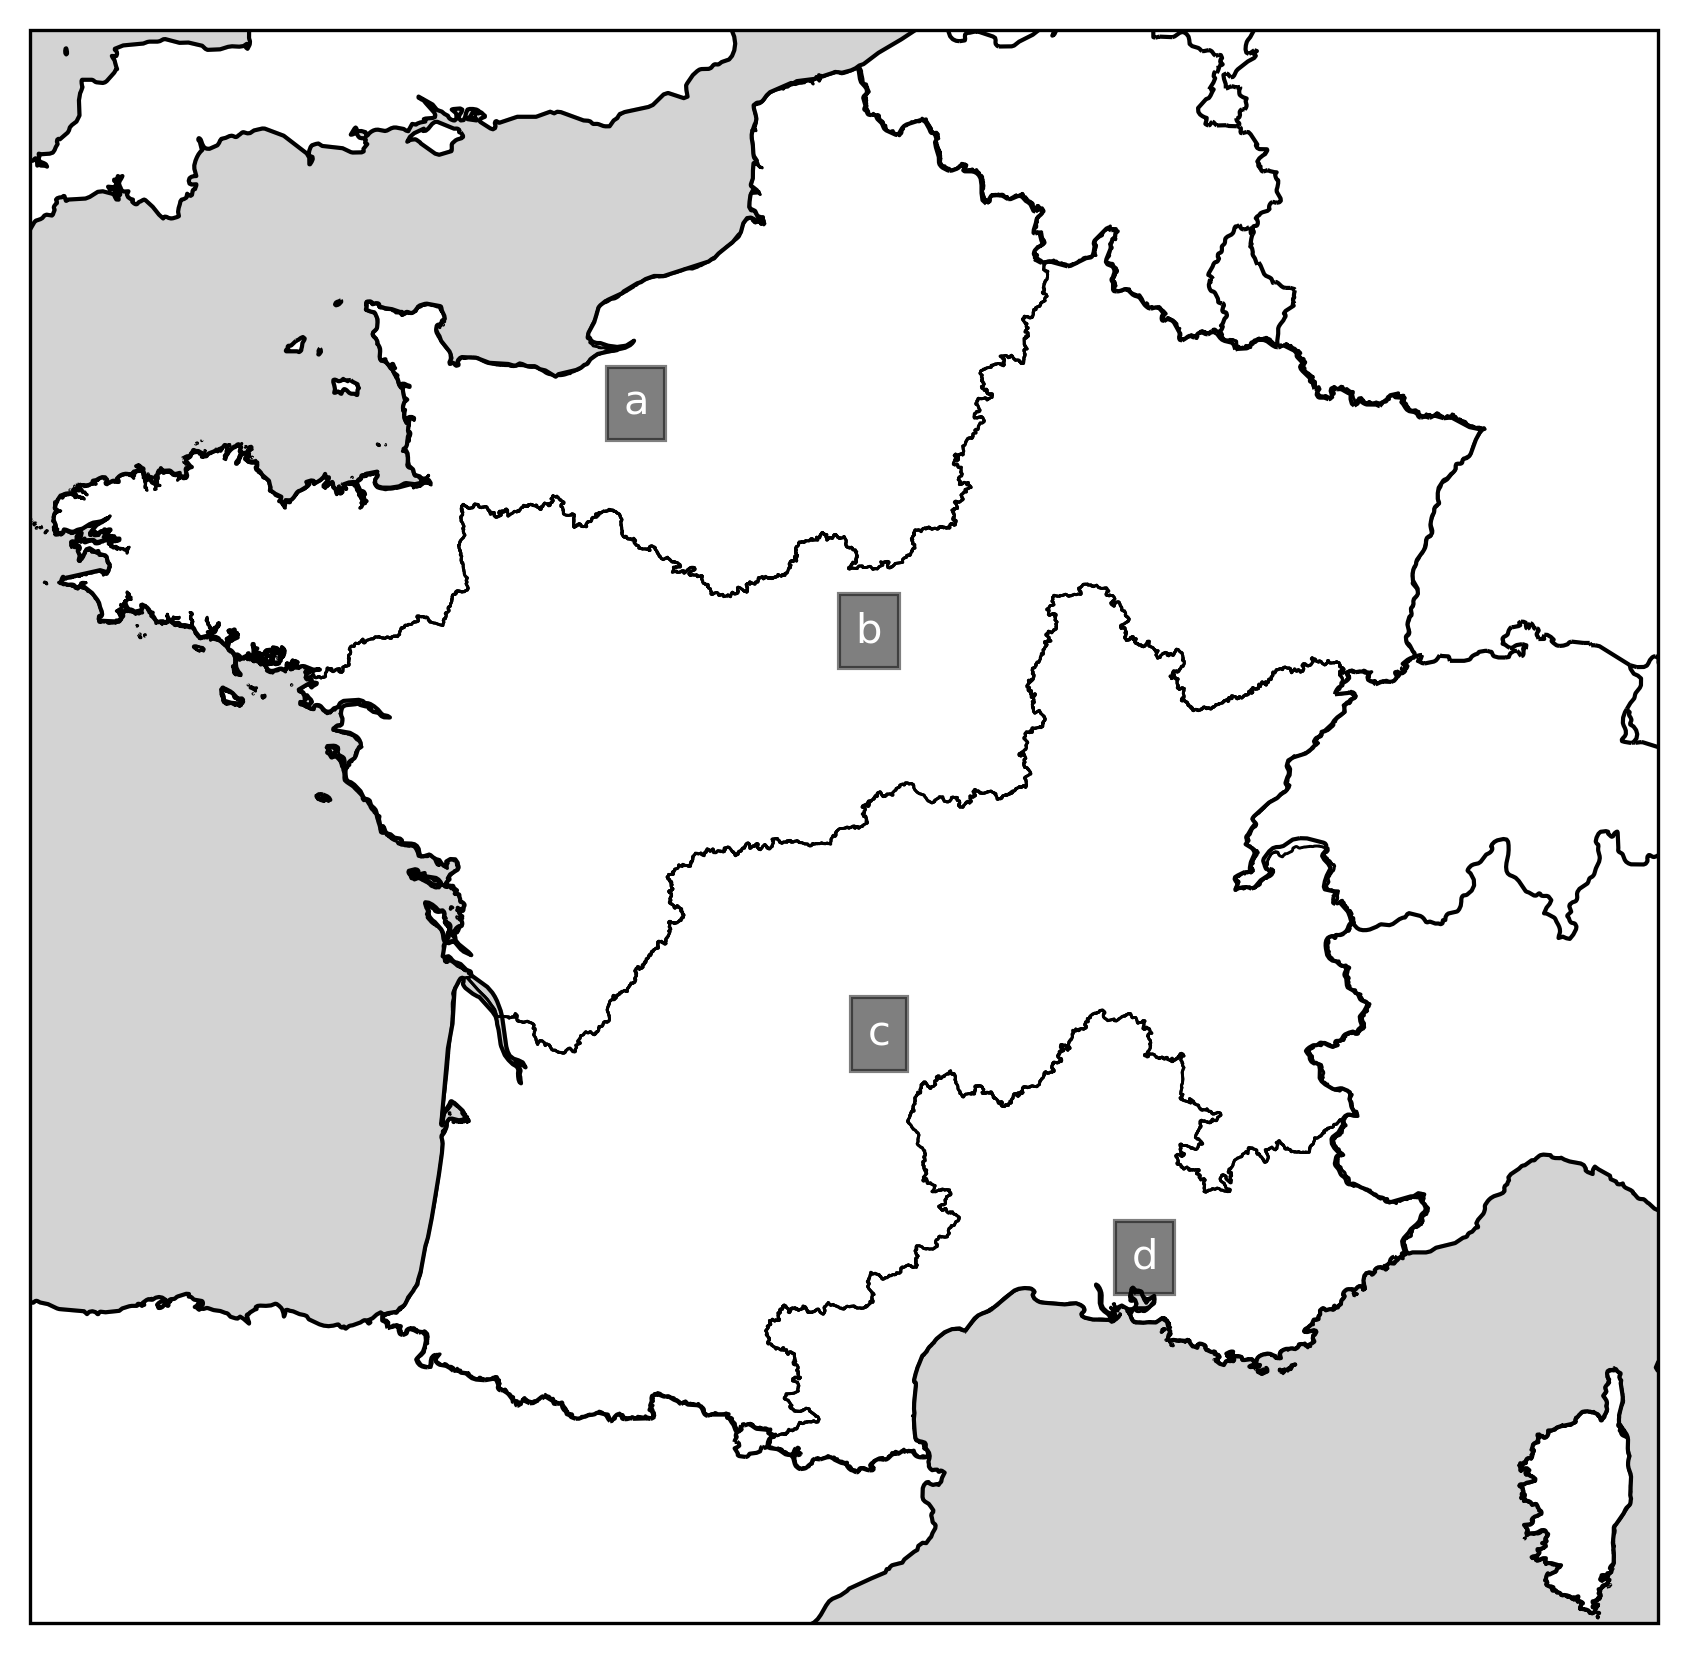
\includegraphics[width=0.32\columnwidth]{figures/zcl_summer.png}
            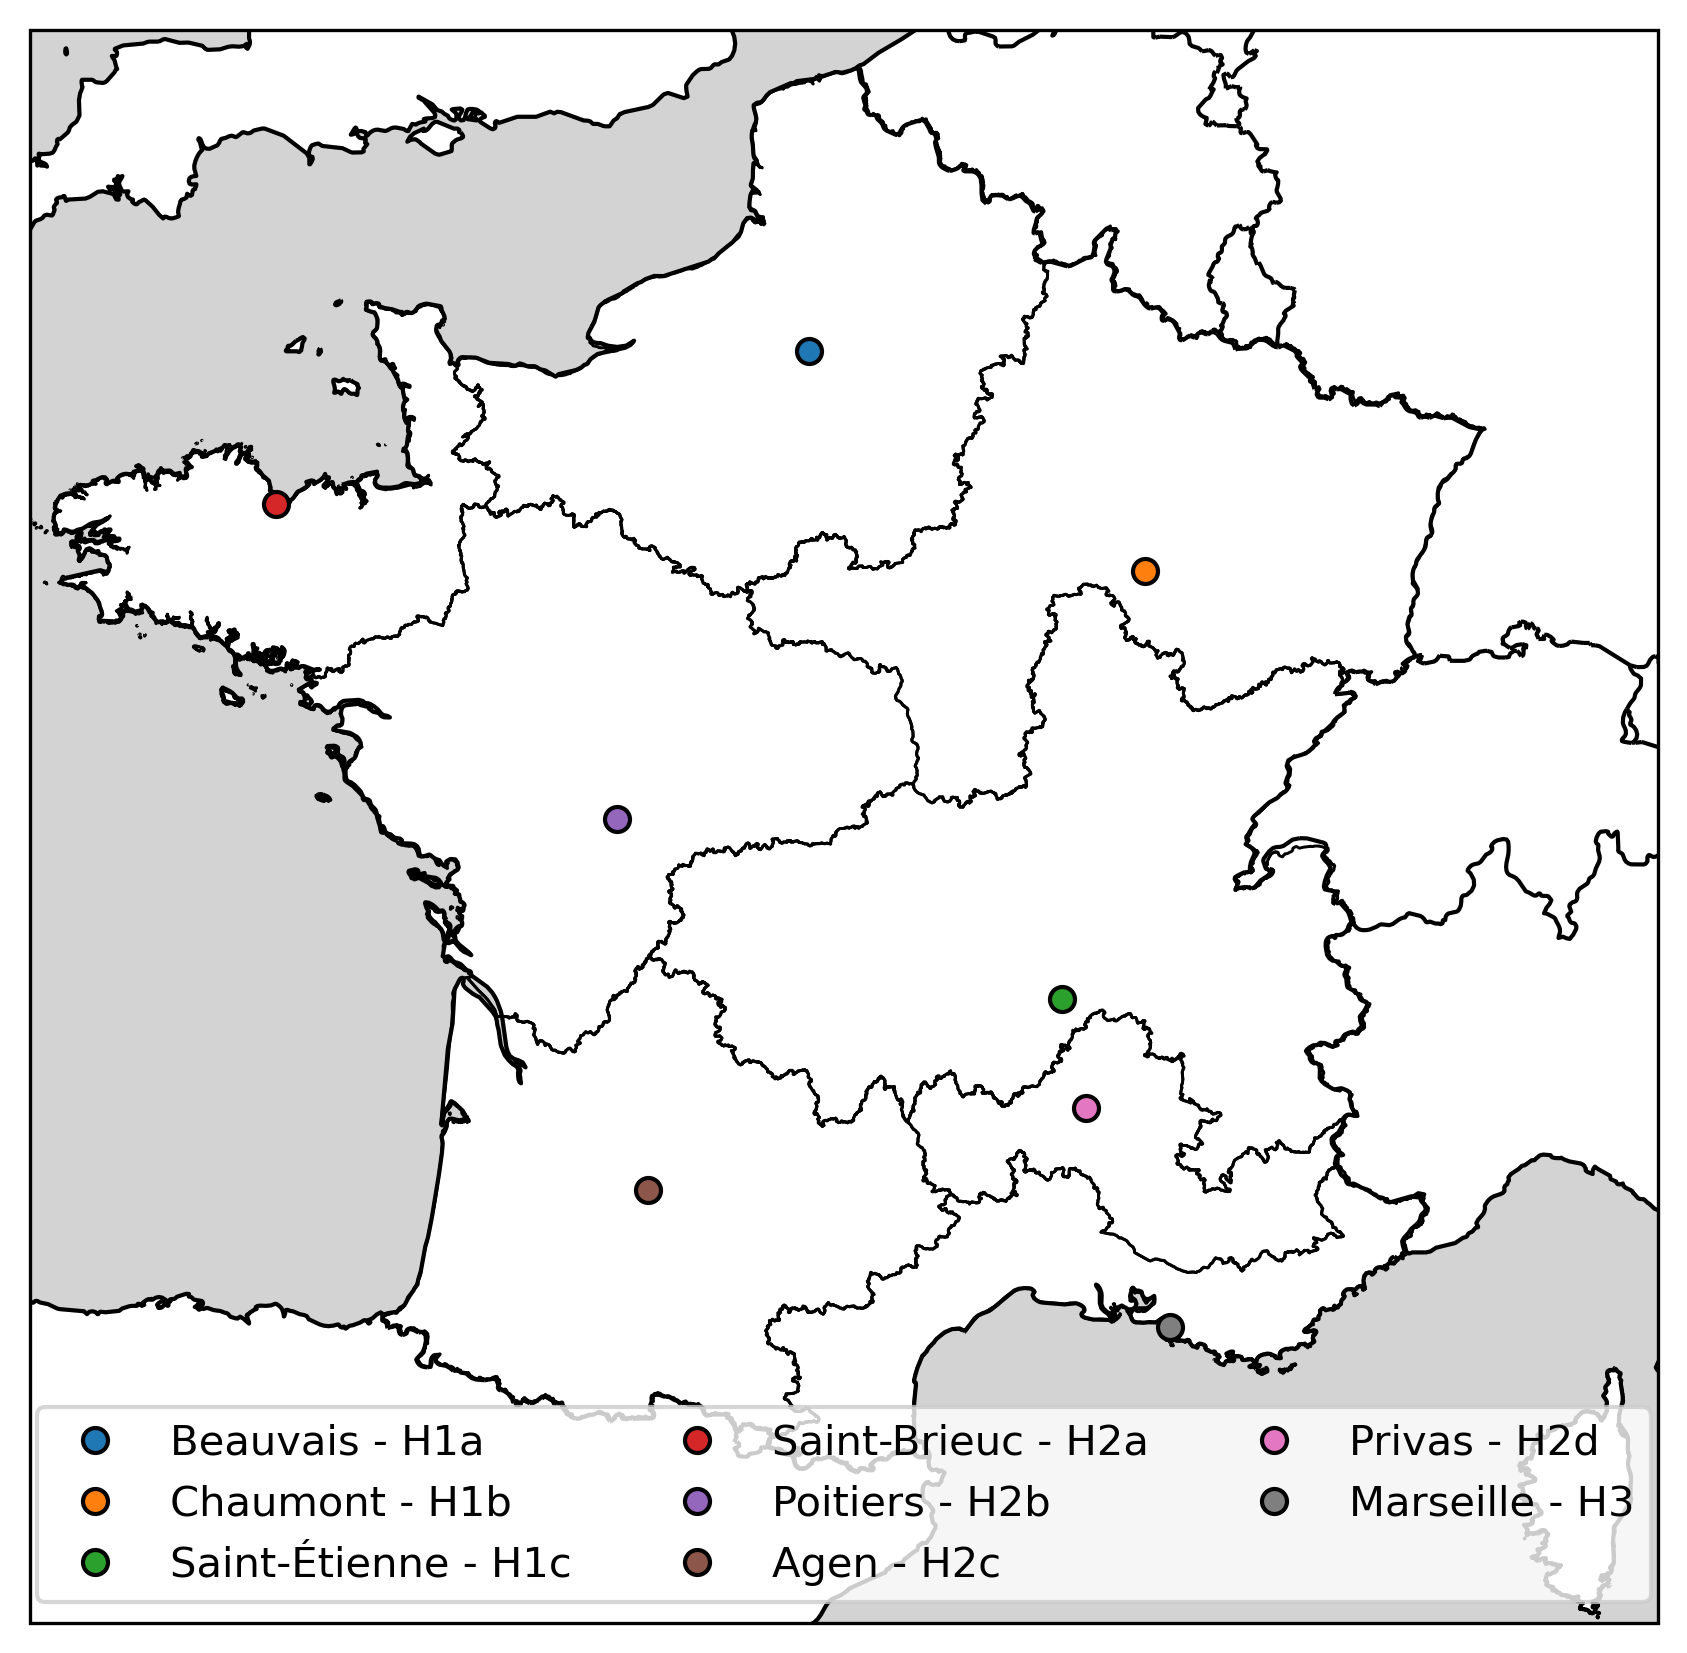
\includegraphics[width=0.32\columnwidth]{figures/zcl.png}
            \caption{\label{fig:zcl} Maps of french climate zones.}
            \begin{quote}
                \vspace{-2mm}
                \small\noindent
                \textbf{(left to right)} Map of \enquote{winter}, \enquote{summer} and combined climate zones. The winter climate zones were defined in a 1988 decree on the thermal characteristics of residential buildings (\cite{jorf_arrete_1988}). Corsica is part of region H3. Summer climate zones were defined in 2000 in parallel with new thermal regulation laws (\cite{jorf_arrete_2000}). The 8 climate zones are a combination of the two zone types (\cite{jorf_arrete_2012}) and the map shows the \enquote{central prefectures} used to define the meteorological data for each zone, as defined in \eqref{eq:pref_centr}. 
                
                 
              \end{quote}
        \end{figure}
        
        % subsubsection french_climate_zones (end)
        \subsubsection{Historical and projection data} % (fold)
        \label{ssub:historical_data}
        
        source des données 
        (\cite{hersbach_era5_2020}, \cite{zippenfenig_open-meteocom_2024})

        periode de reference 2000-2020

        projection : \cite{sauquet_explore2_2021} cf DRIAS

        calcul des temperatures infra journalières 

        calcul des flux solaires infra journaliers (\cite{knight_methodology_1991}, \cite{chow_new_2007})
        % subsubsection historical_data (end)

        \subsubsection{Standard weather data} % (fold)
        \label{ssub:standard_weather_data}
        
        pour economiser en temps de calcul, a chaque fois ets auf mention contraire, une année moyenne des périodes, définies tel que
        % subsubsection standard_weather_data (end)
    
    % subsection weather_data (end)

    \subsection{Behaviour definition} % (fold)
    \label{sub:behaviour_definition}


    
    % subsection behaviour_definition (end)
% section rc (end)

\clearpage
\section{Interactions between summer and winter comfort}
\label{sec:inter}

    \subsection{Single renovation actions} % (fold)
    \label{sub:single_renovation_actions}
    
    actions monogestes : grande part des travaux de renovations (\cite{ademe_typologie_2019}, \cite{onre_renovation_2022})


    liste des actions et details du choix (\cite{i4ce_trajectoires_2023}, \cite{peuportier_resiliance_2023})

    plus choix des typologies, des climats

        \subsubsection{Roof insulation} % (fold)
        \label{ssub:roof_insulation}
        
            detailler les caractéristiques propre à ce type de rénovation, pourquoi les gens l'ont bcp fait etc. 

            commenter l'interaction (\ref{fig:roof_init})

            \begin{figure}[ht]
                \centering
                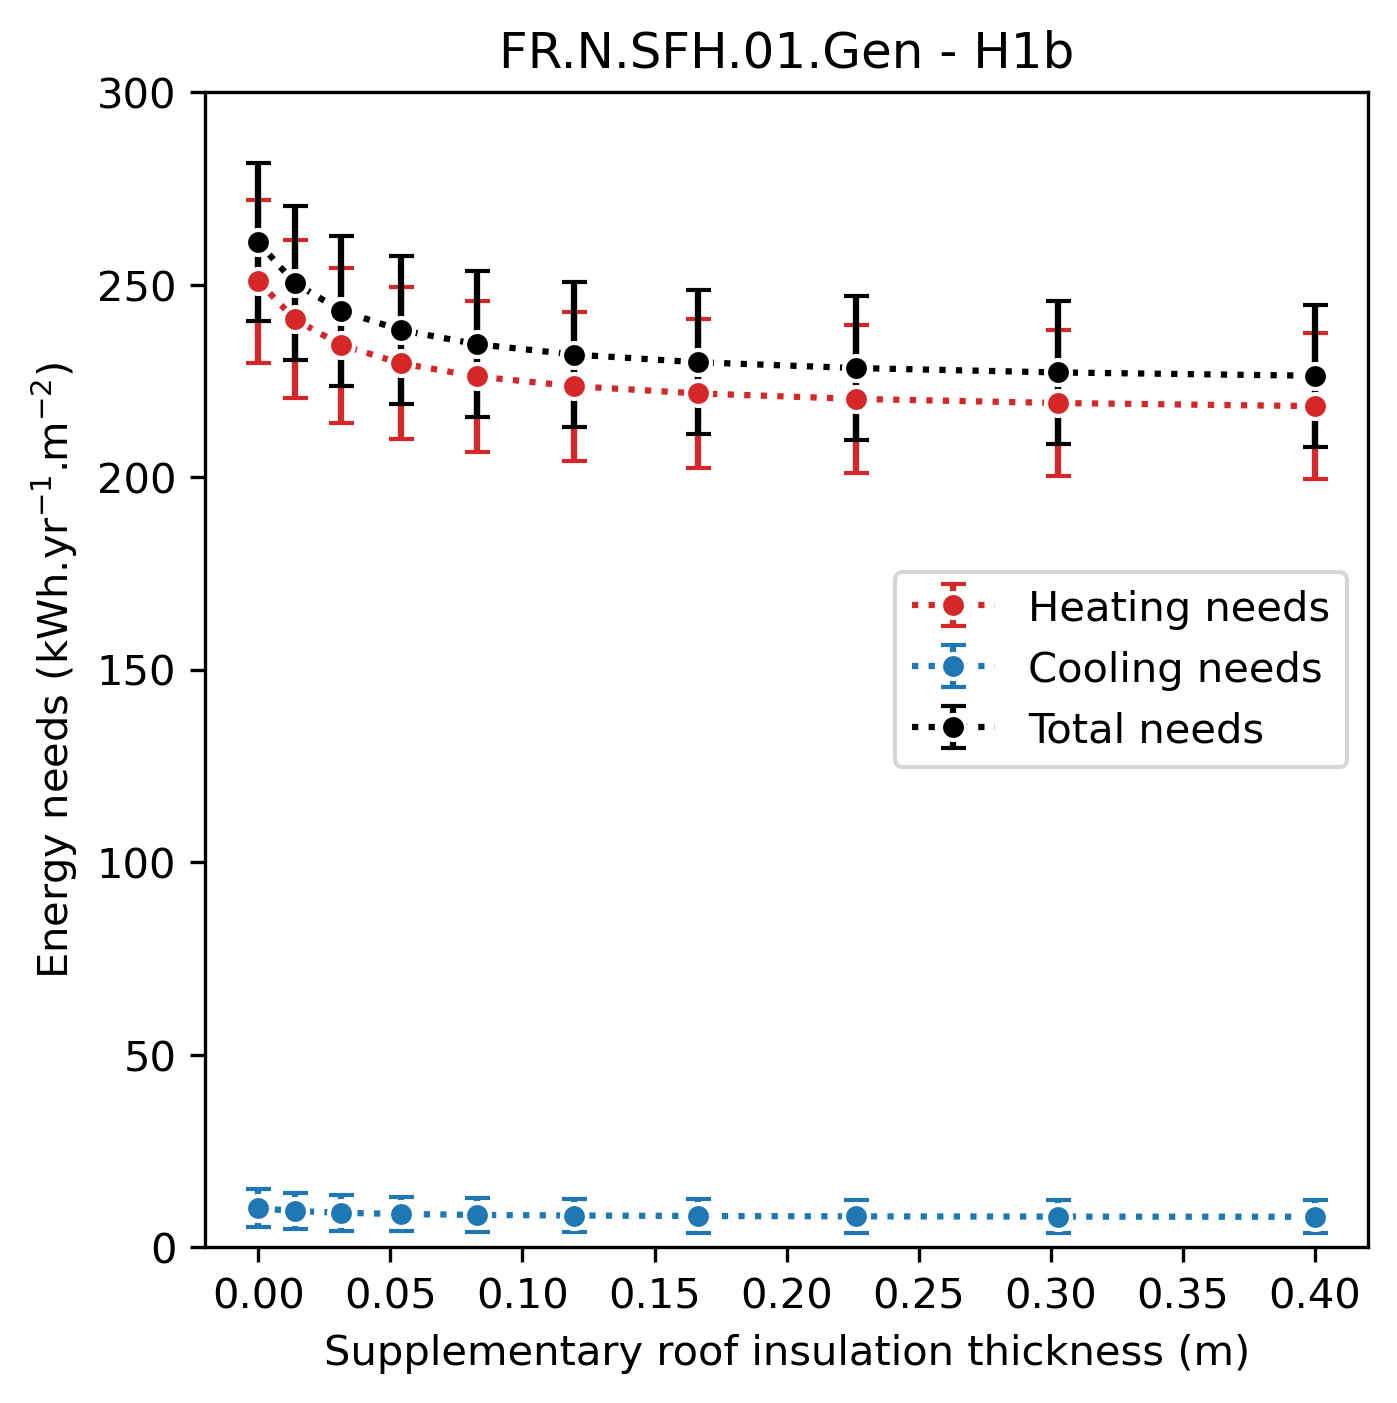
\includegraphics[width=0.32\columnwidth]{figures/roof_FR.N.SFH.01.Gen_H1b_conventionnel_th-bce_2020_2000-2020.png}
                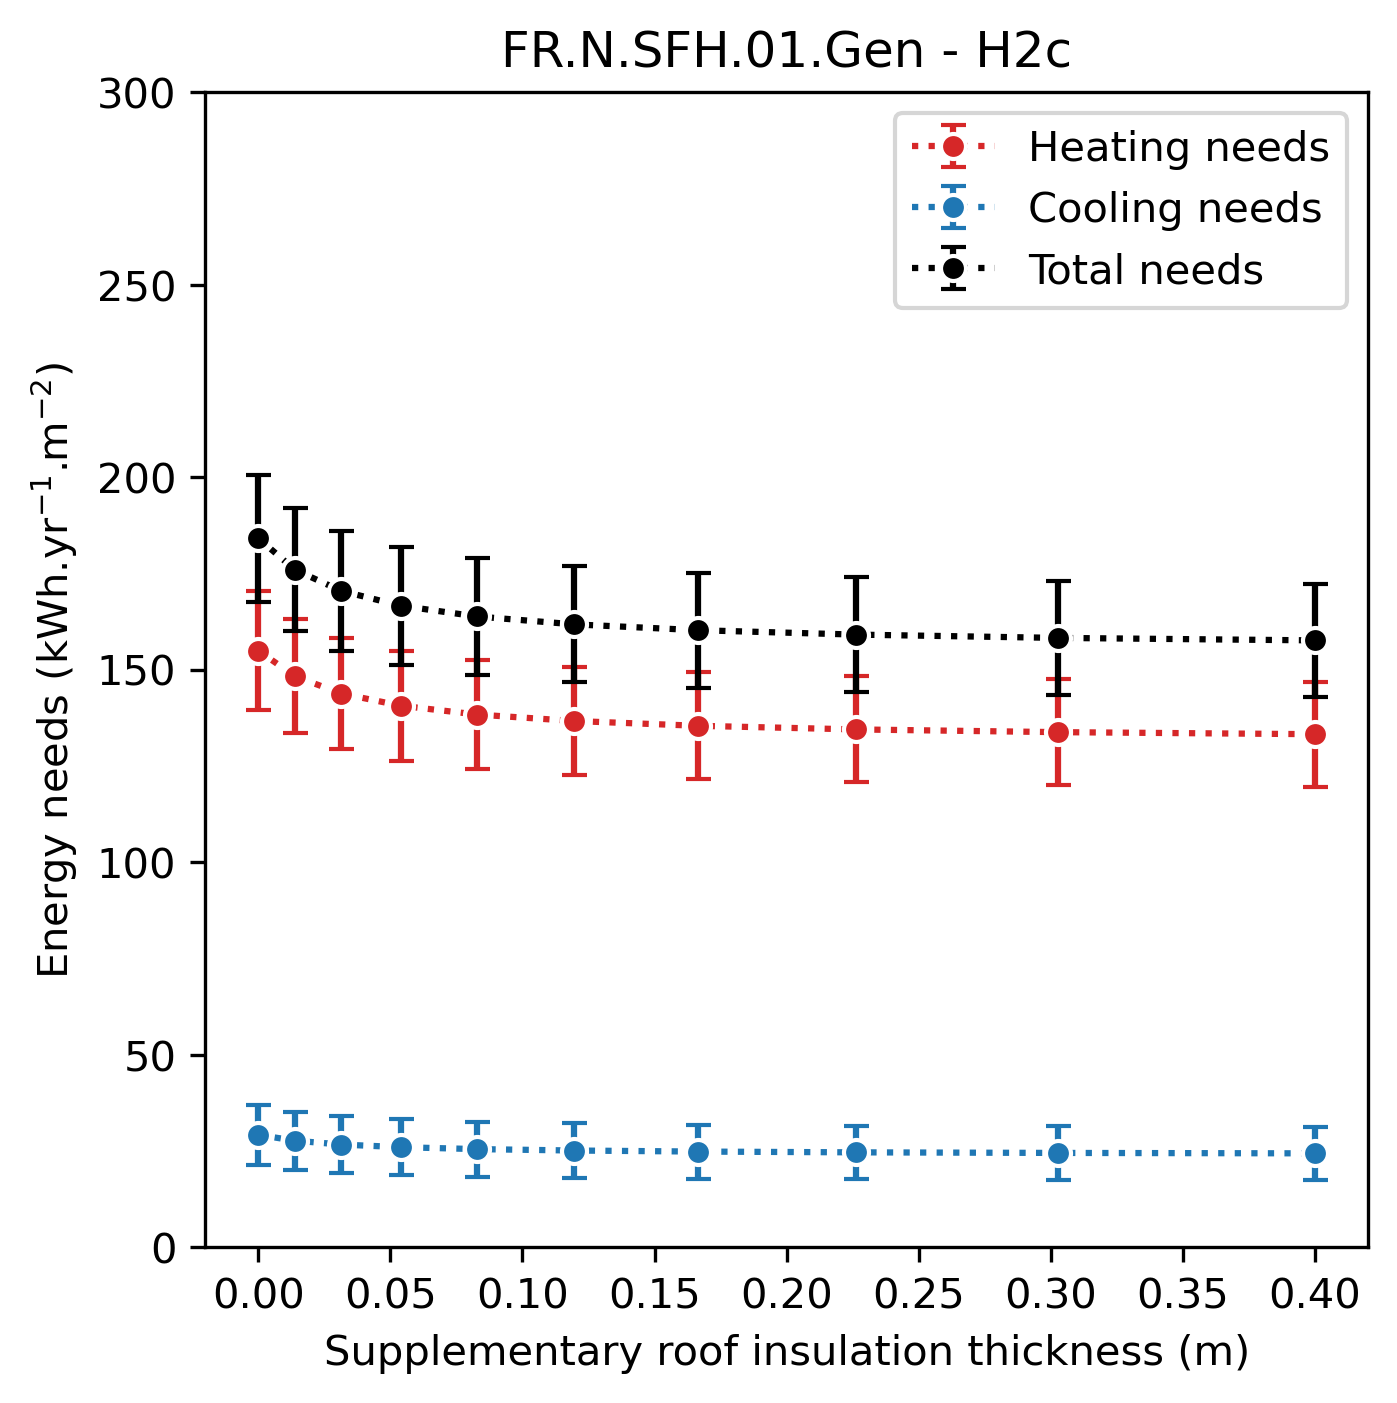
\includegraphics[width=0.32\columnwidth]{figures/roof_FR.N.SFH.01.Gen_H2c_conventionnel_th-bce_2020_2000-2020.png}
                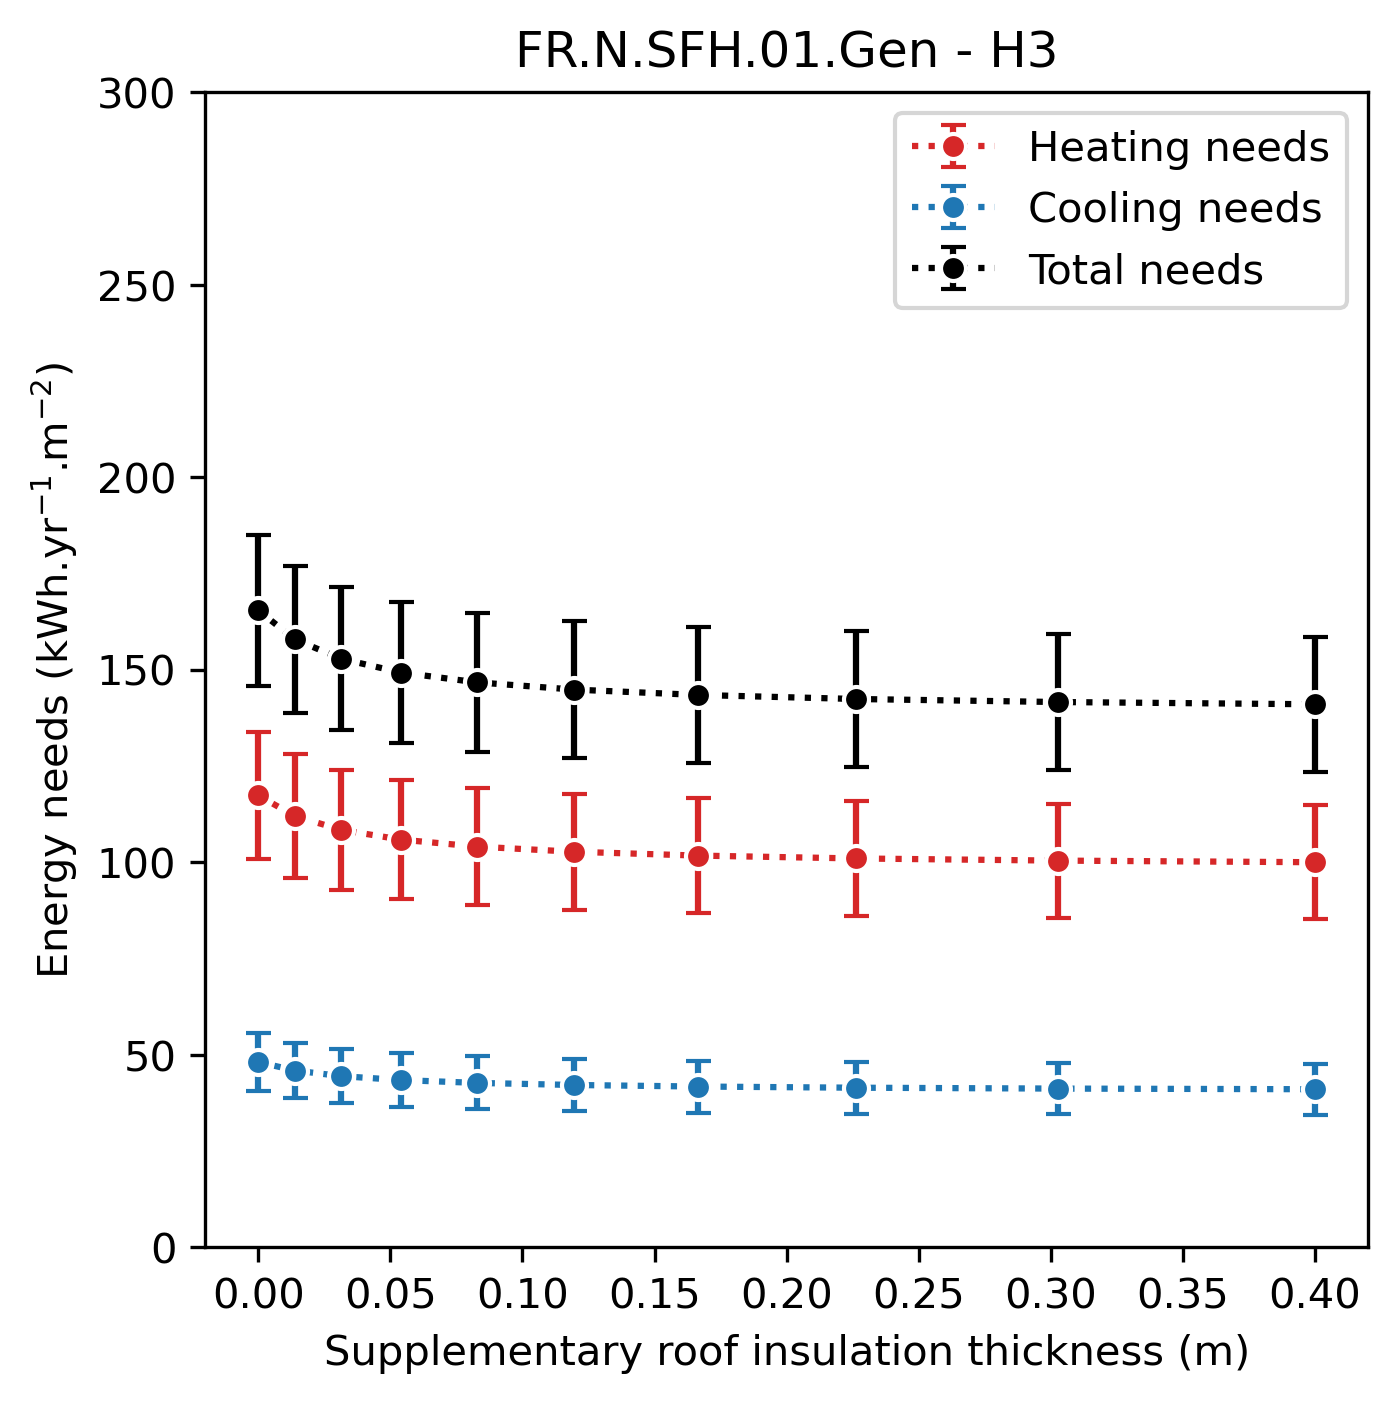
\includegraphics[width=0.32\columnwidth]{figures/roof_FR.N.SFH.01.Gen_H3_conventionnel_th-bce_2020_2000-2020.png}\\
                % 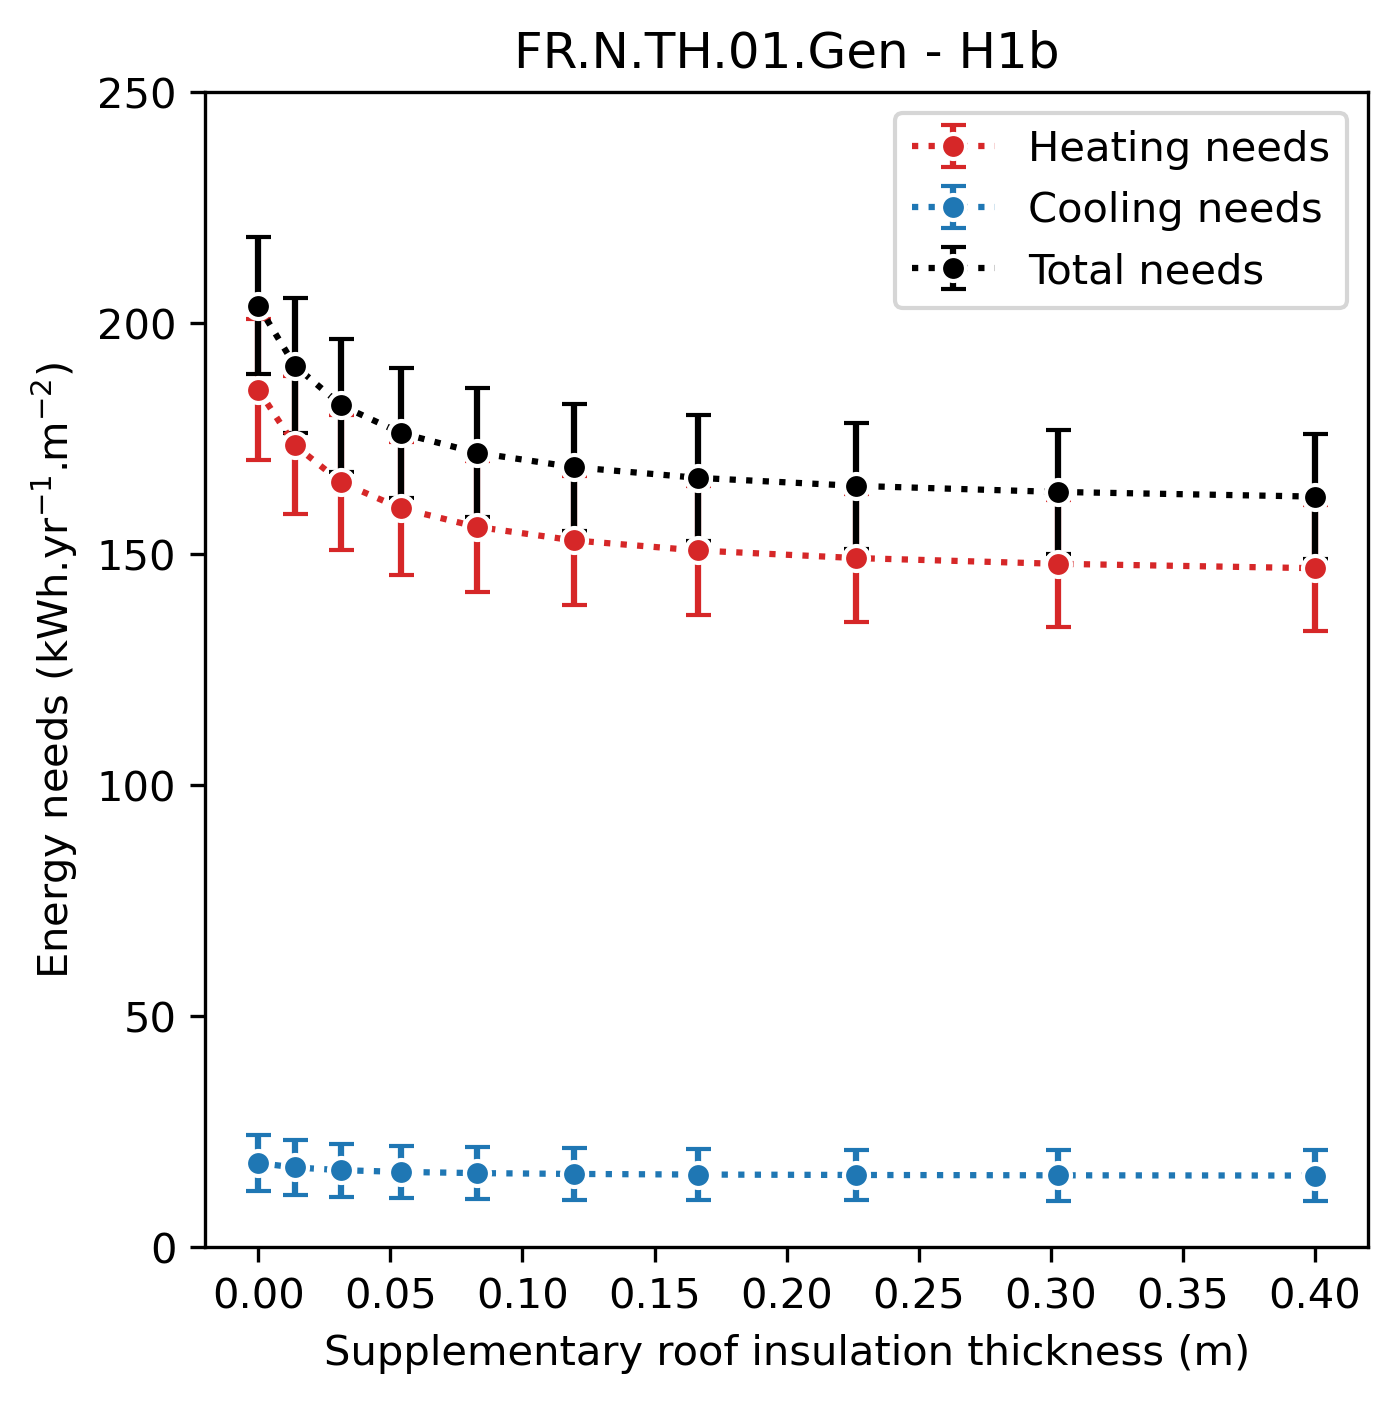
\includegraphics[width=0.32\columnwidth]{figures/roof_FR.N.TH.01.Gen_H1b_conventionnel_th-bce_2020_2000-2020.png}
                % 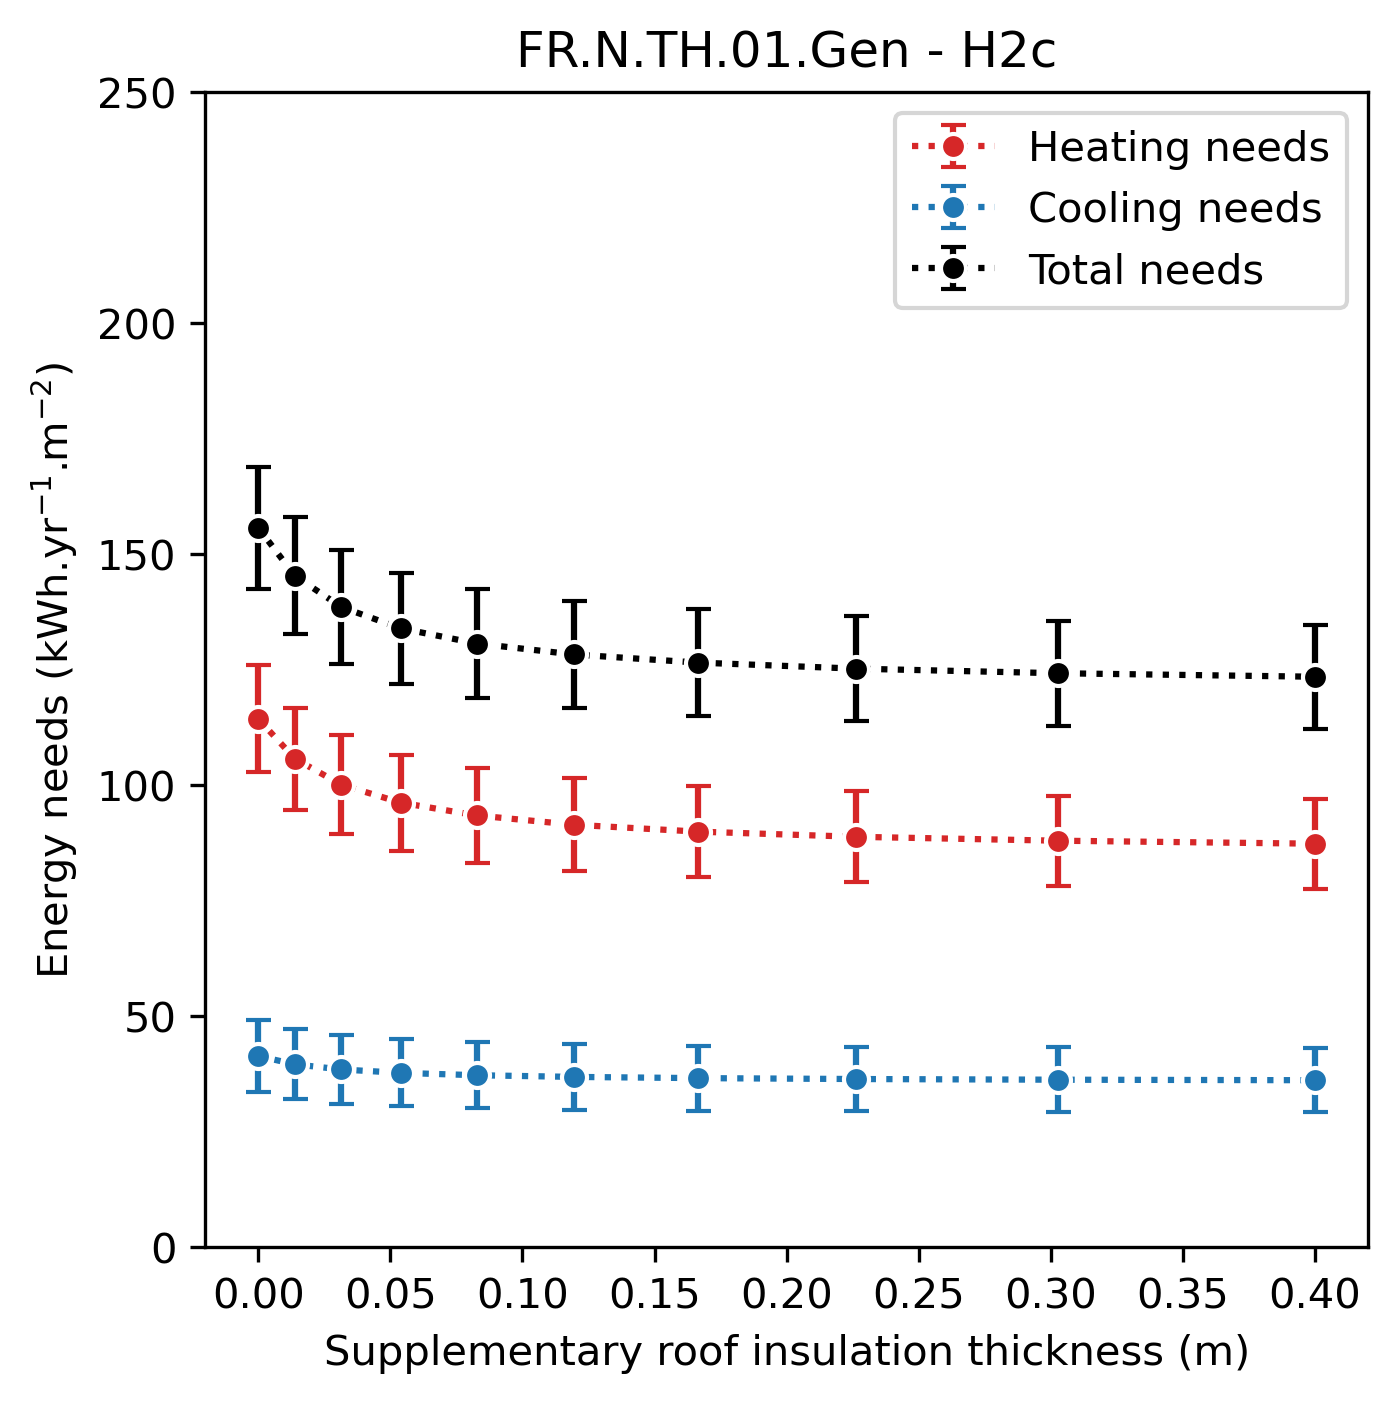
\includegraphics[width=0.32\columnwidth]{figures/roof_FR.N.TH.01.Gen_H2c_conventionnel_th-bce_2020_2000-2020.png}
                % 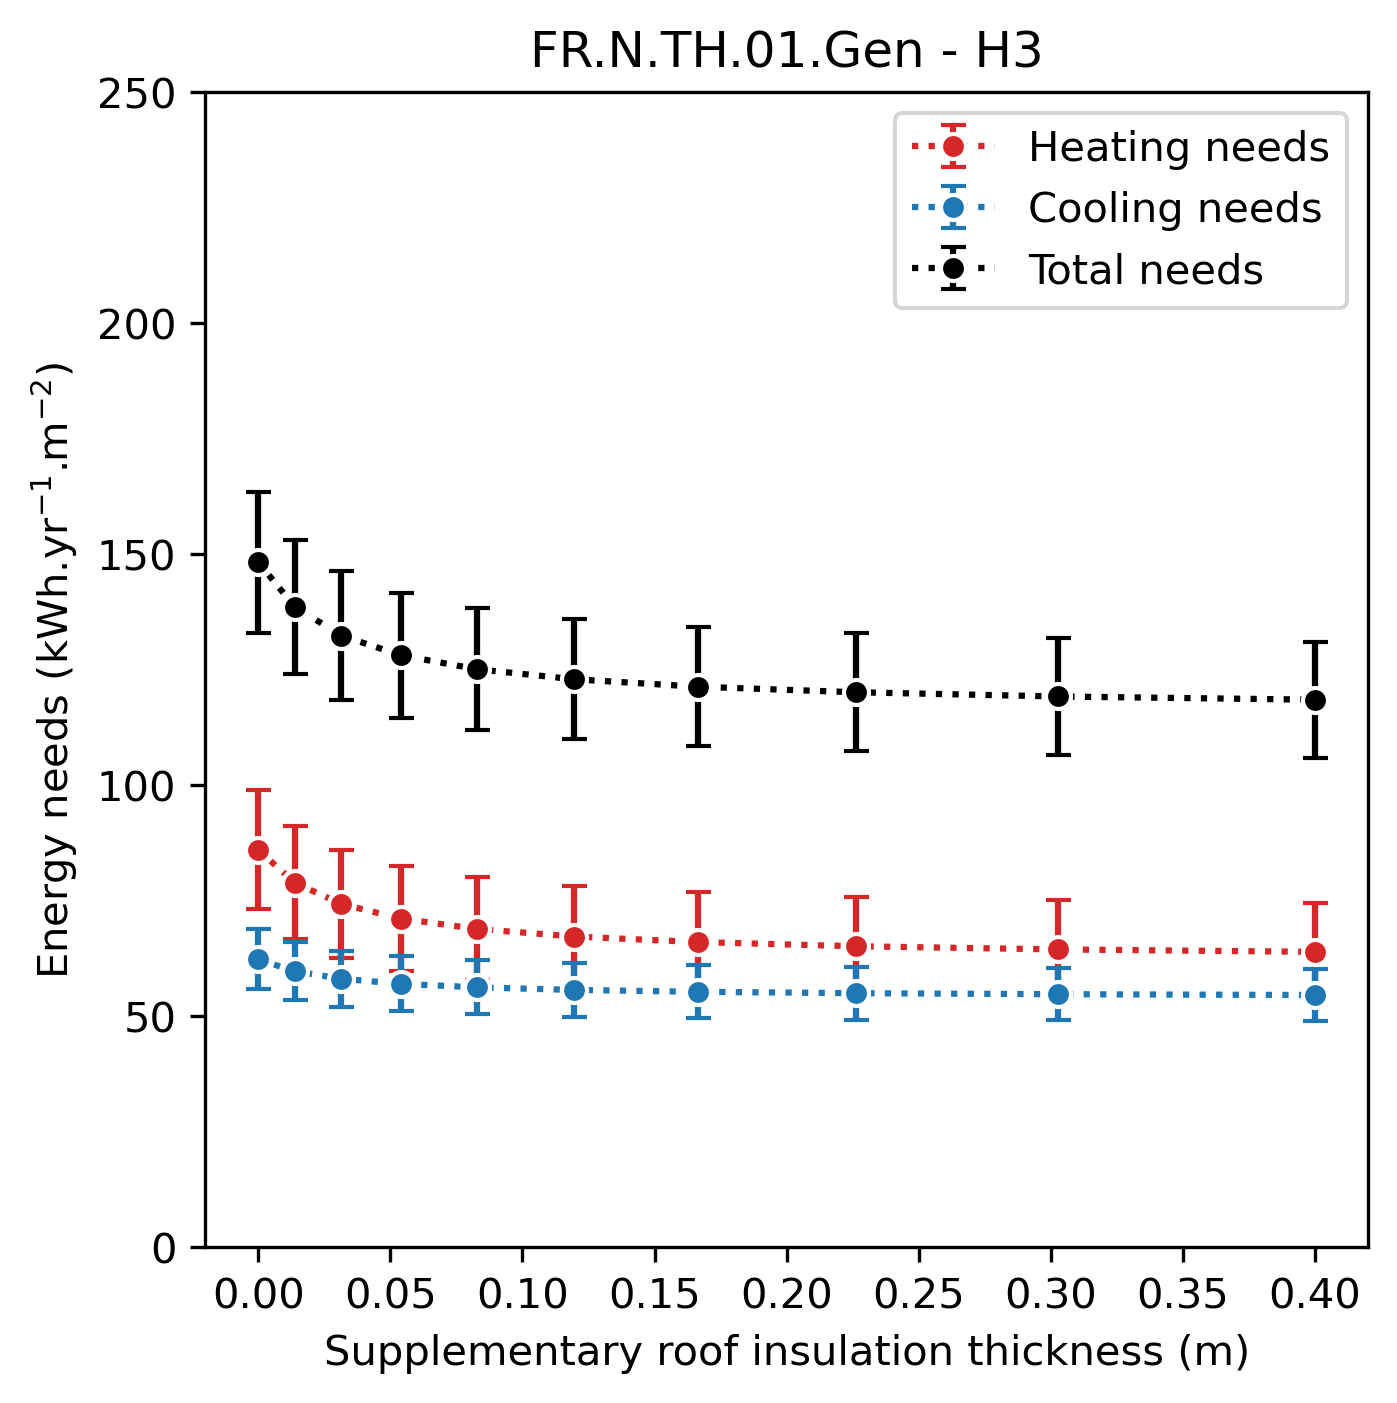
\includegraphics[width=0.32\columnwidth]{figures/roof_FR.N.TH.01.Gen_H3_conventionnel_th-bce_2020_2000-2020.png}\\
                % 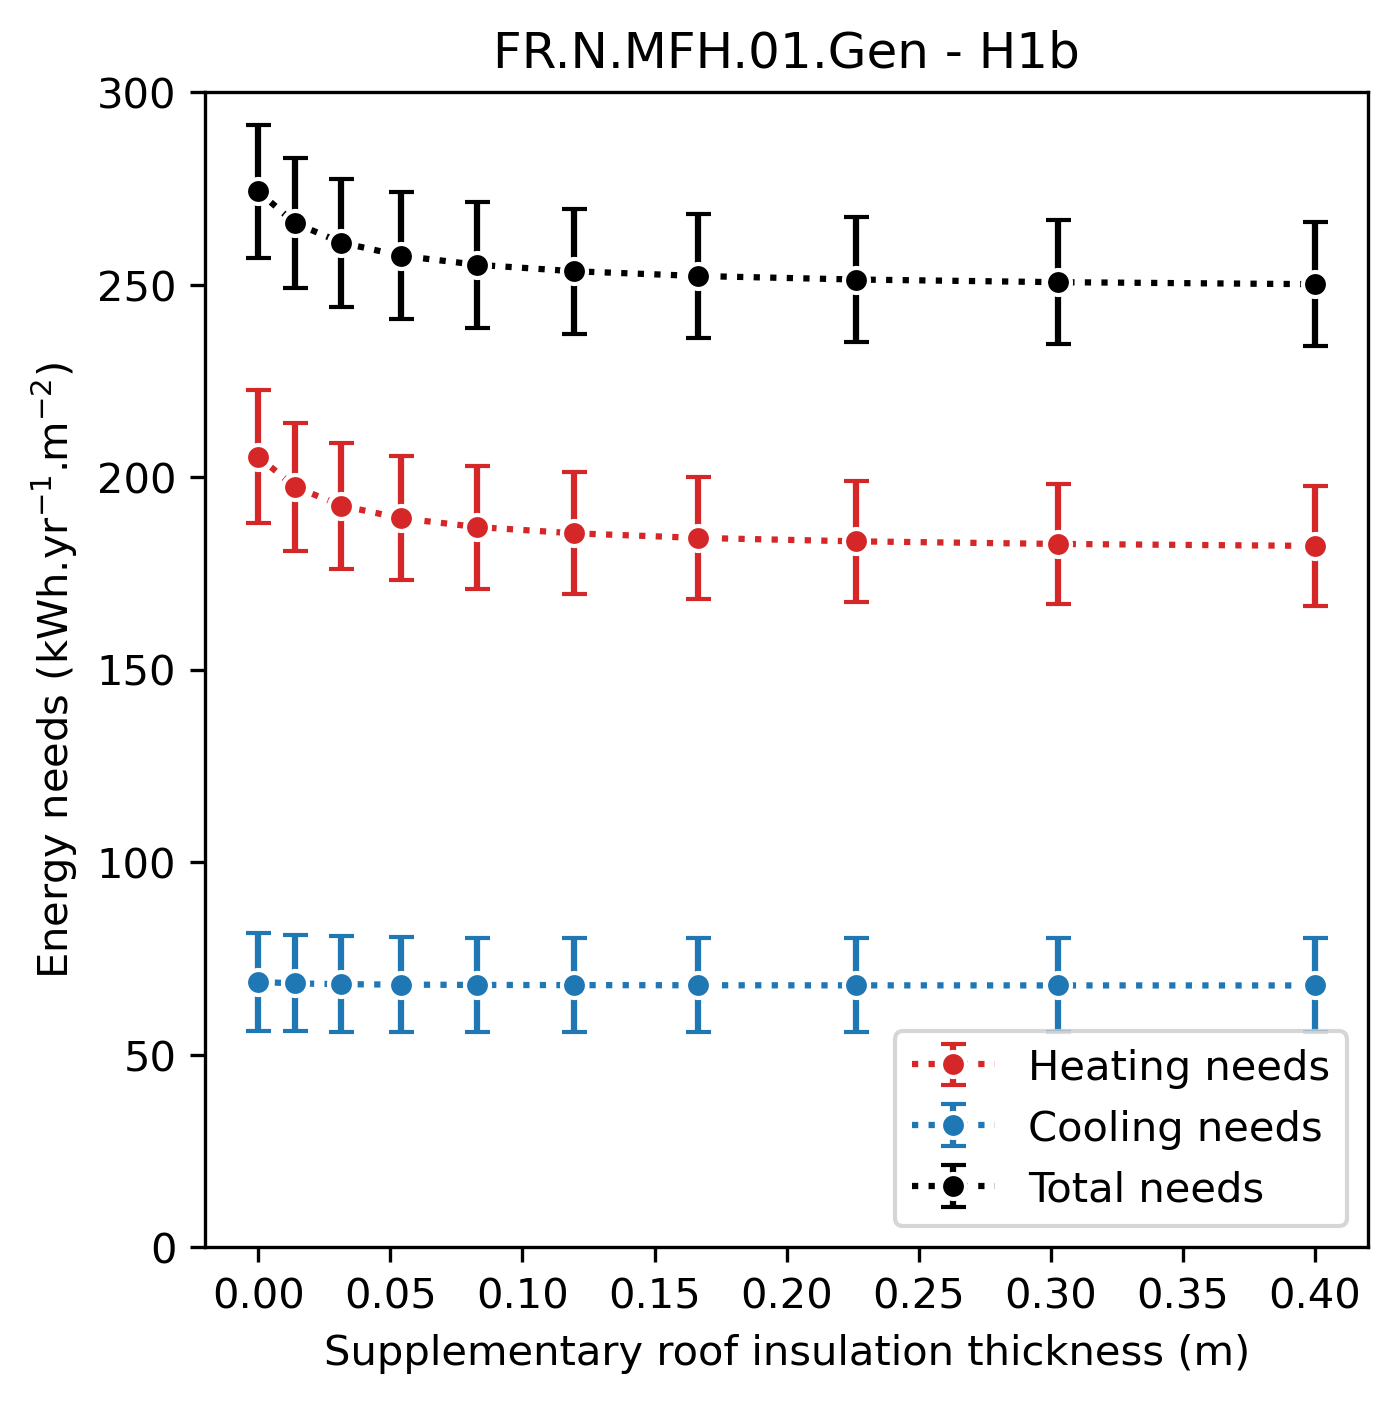
\includegraphics[width=0.32\columnwidth]{figures/roof_FR.N.MFH.01.Gen_H1b_conventionnel_th-bce_2020_2000-2020.png}
                % 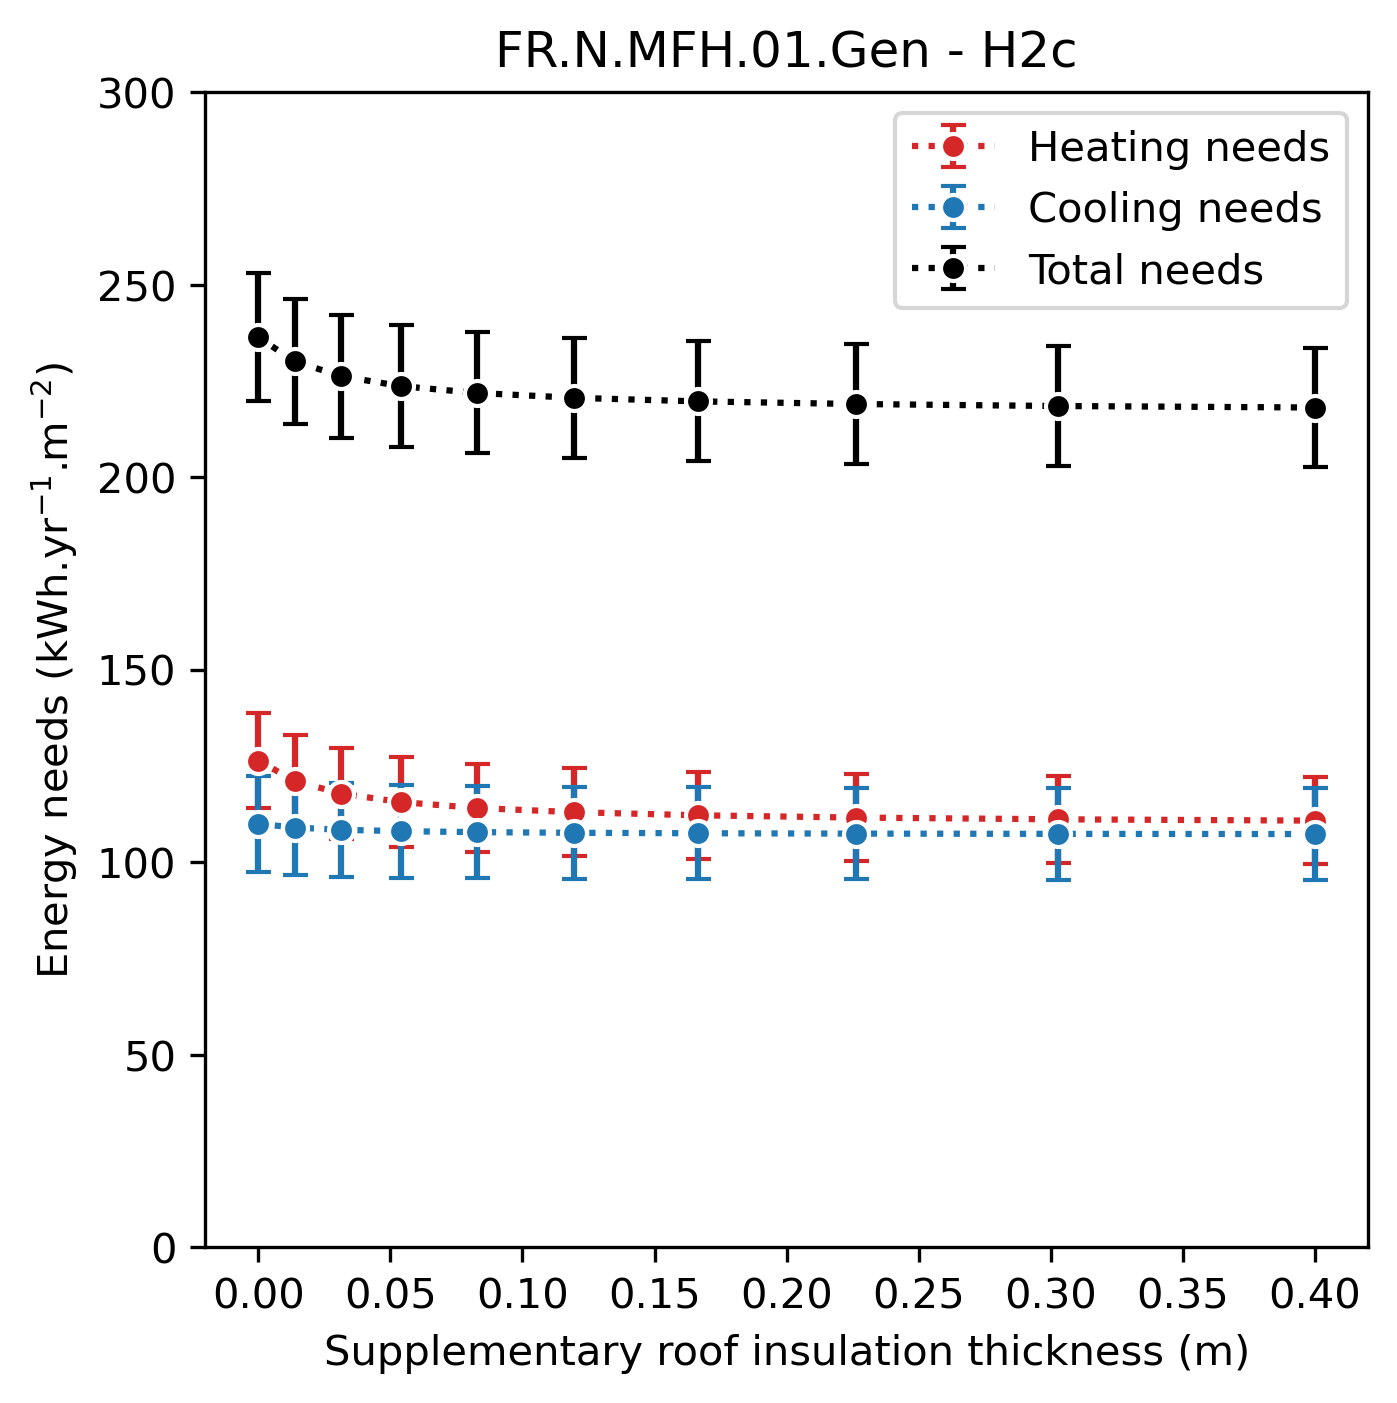
\includegraphics[width=0.32\columnwidth]{figures/roof_FR.N.MFH.01.Gen_H2c_conventionnel_th-bce_2020_2000-2020.png}
                % 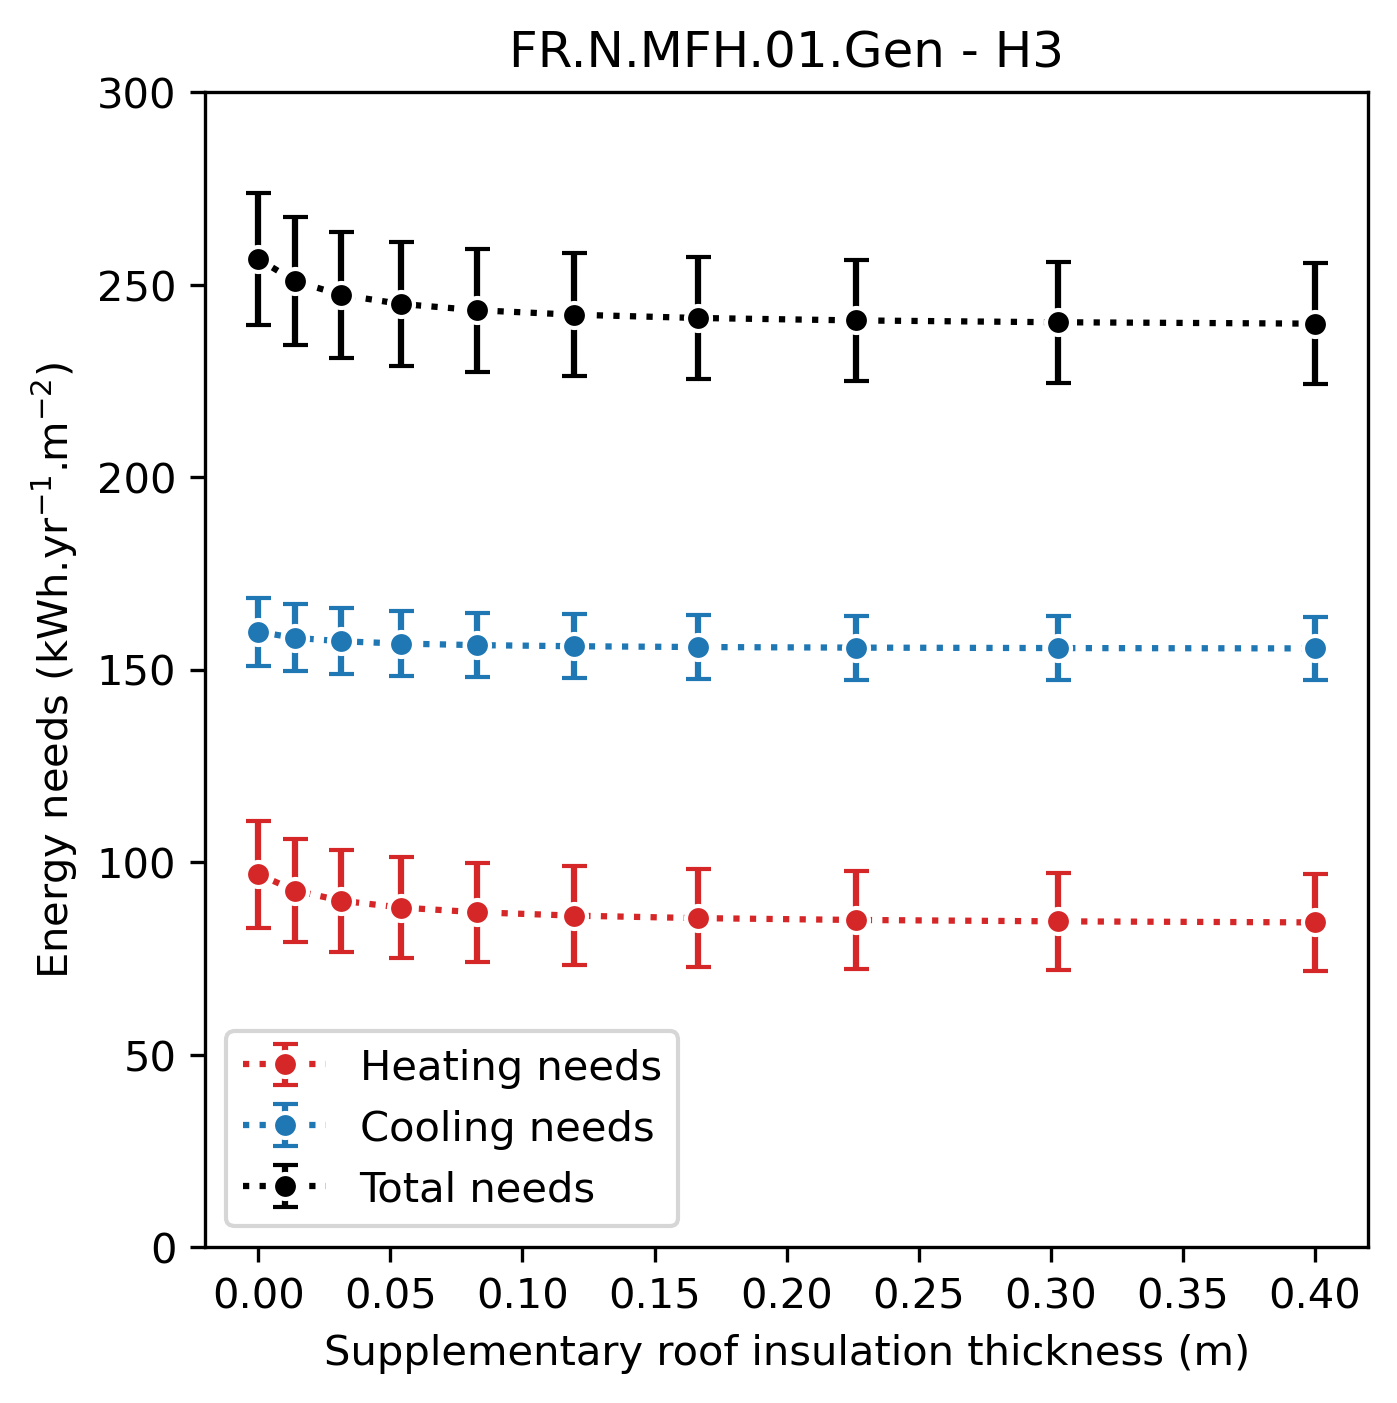
\includegraphics[width=0.32\columnwidth]{figures/roof_FR.N.MFH.01.Gen_H3_conventionnel_th-bce_2020_2000-2020.png}\\
                % 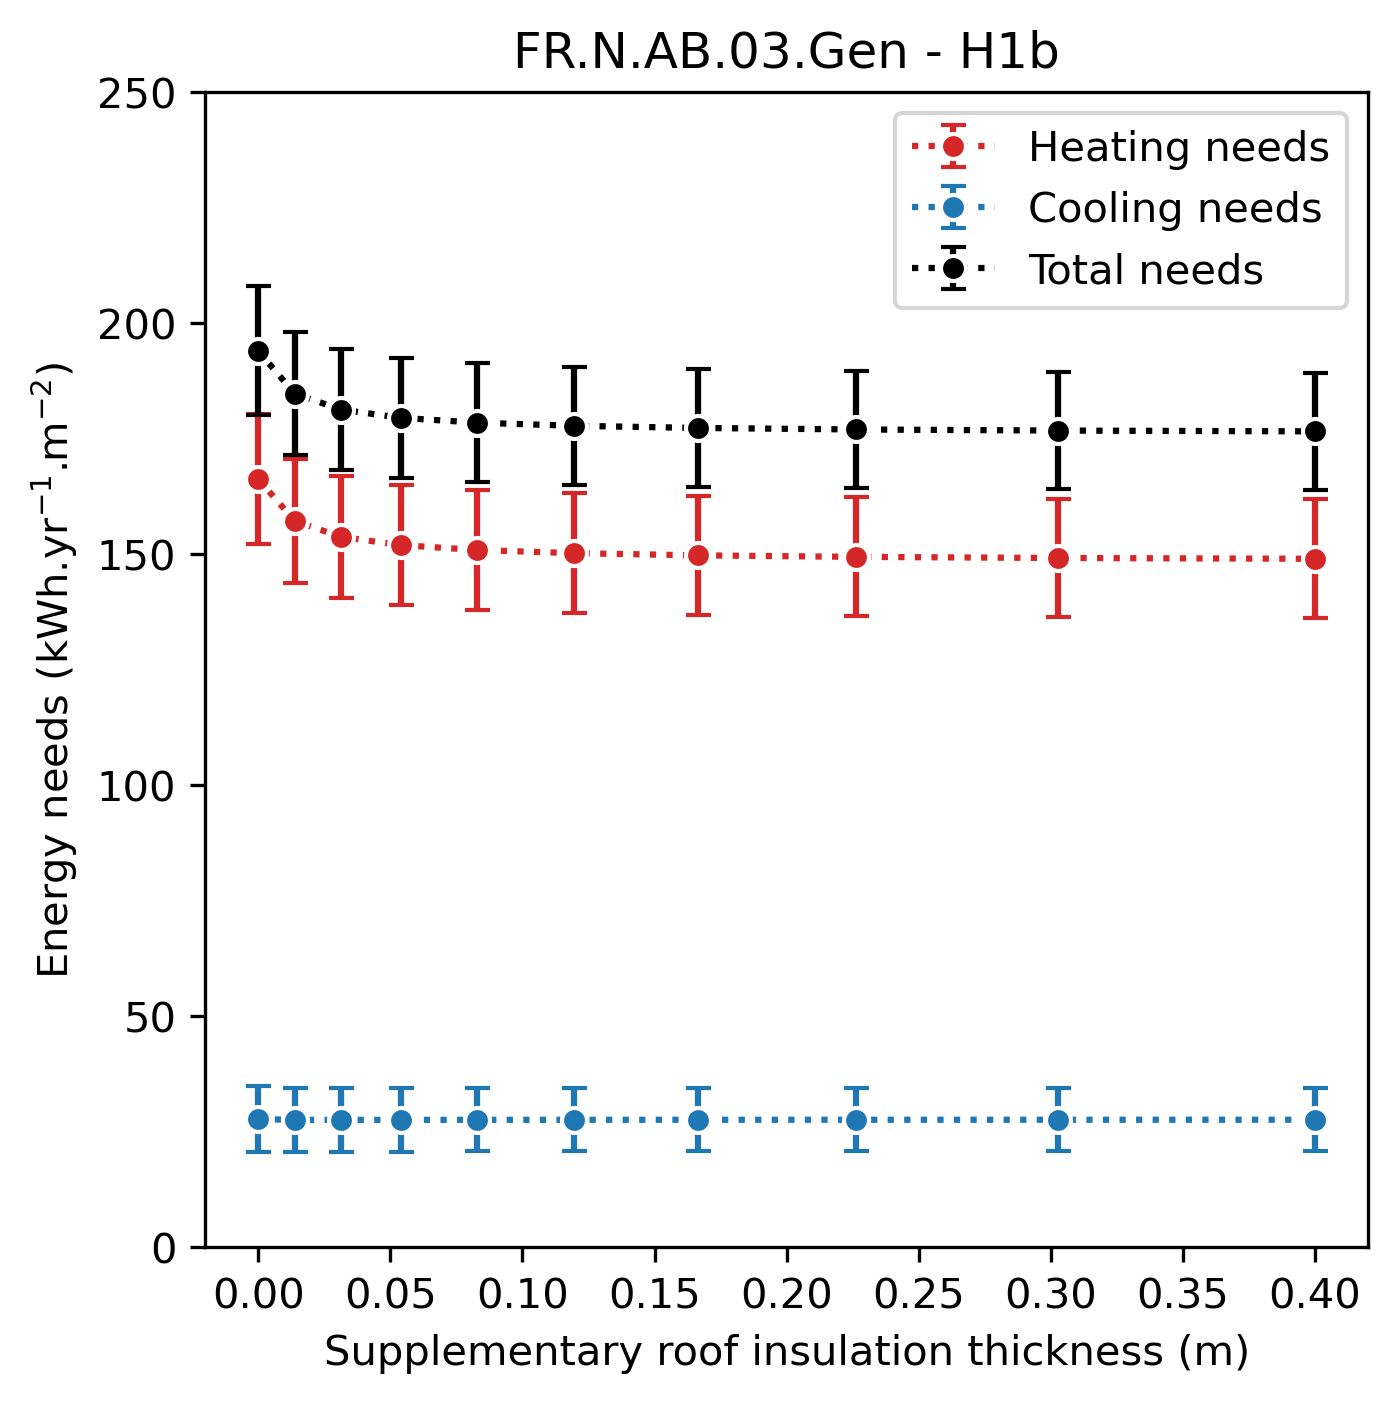
\includegraphics[width=0.32\columnwidth]{figures/roof_FR.N.AB.03.Gen_H1b_conventionnel_th-bce_2020_2000-2020.png}
                % 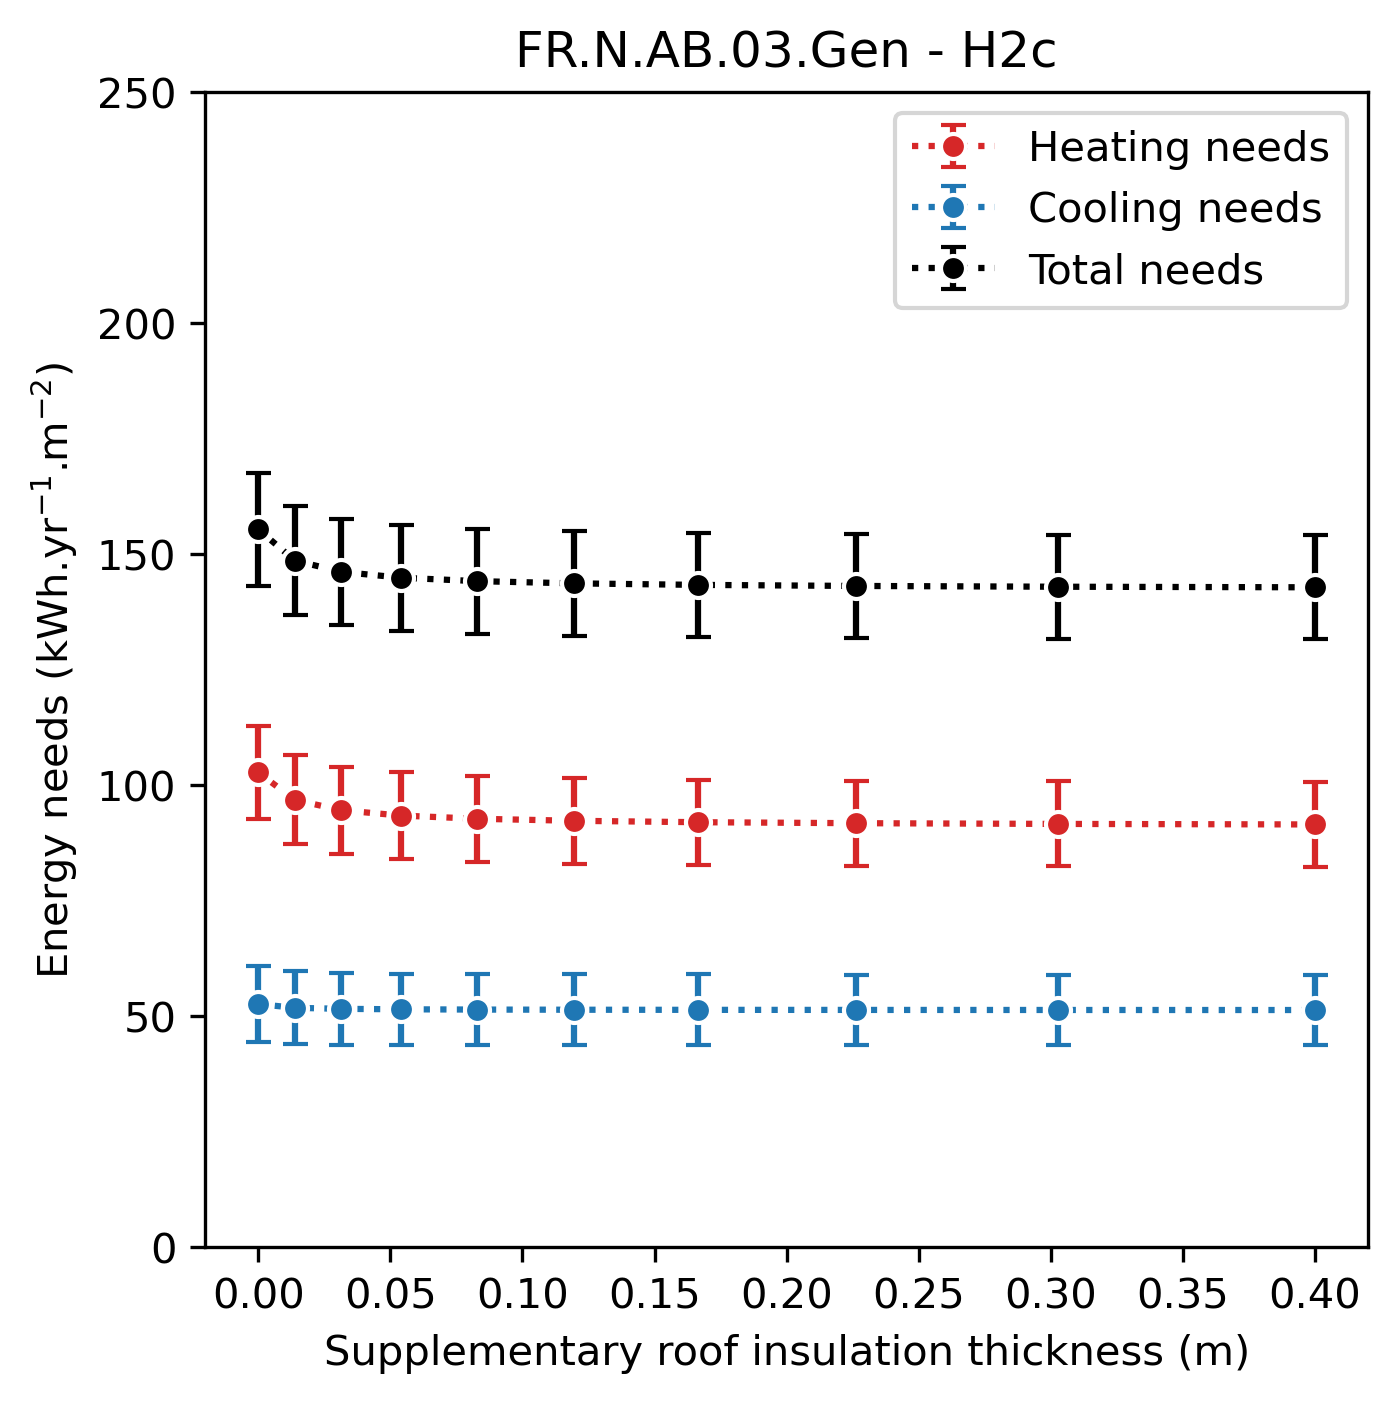
\includegraphics[width=0.32\columnwidth]{figures/roof_FR.N.AB.03.Gen_H2c_conventionnel_th-bce_2020_2000-2020.png}
                % 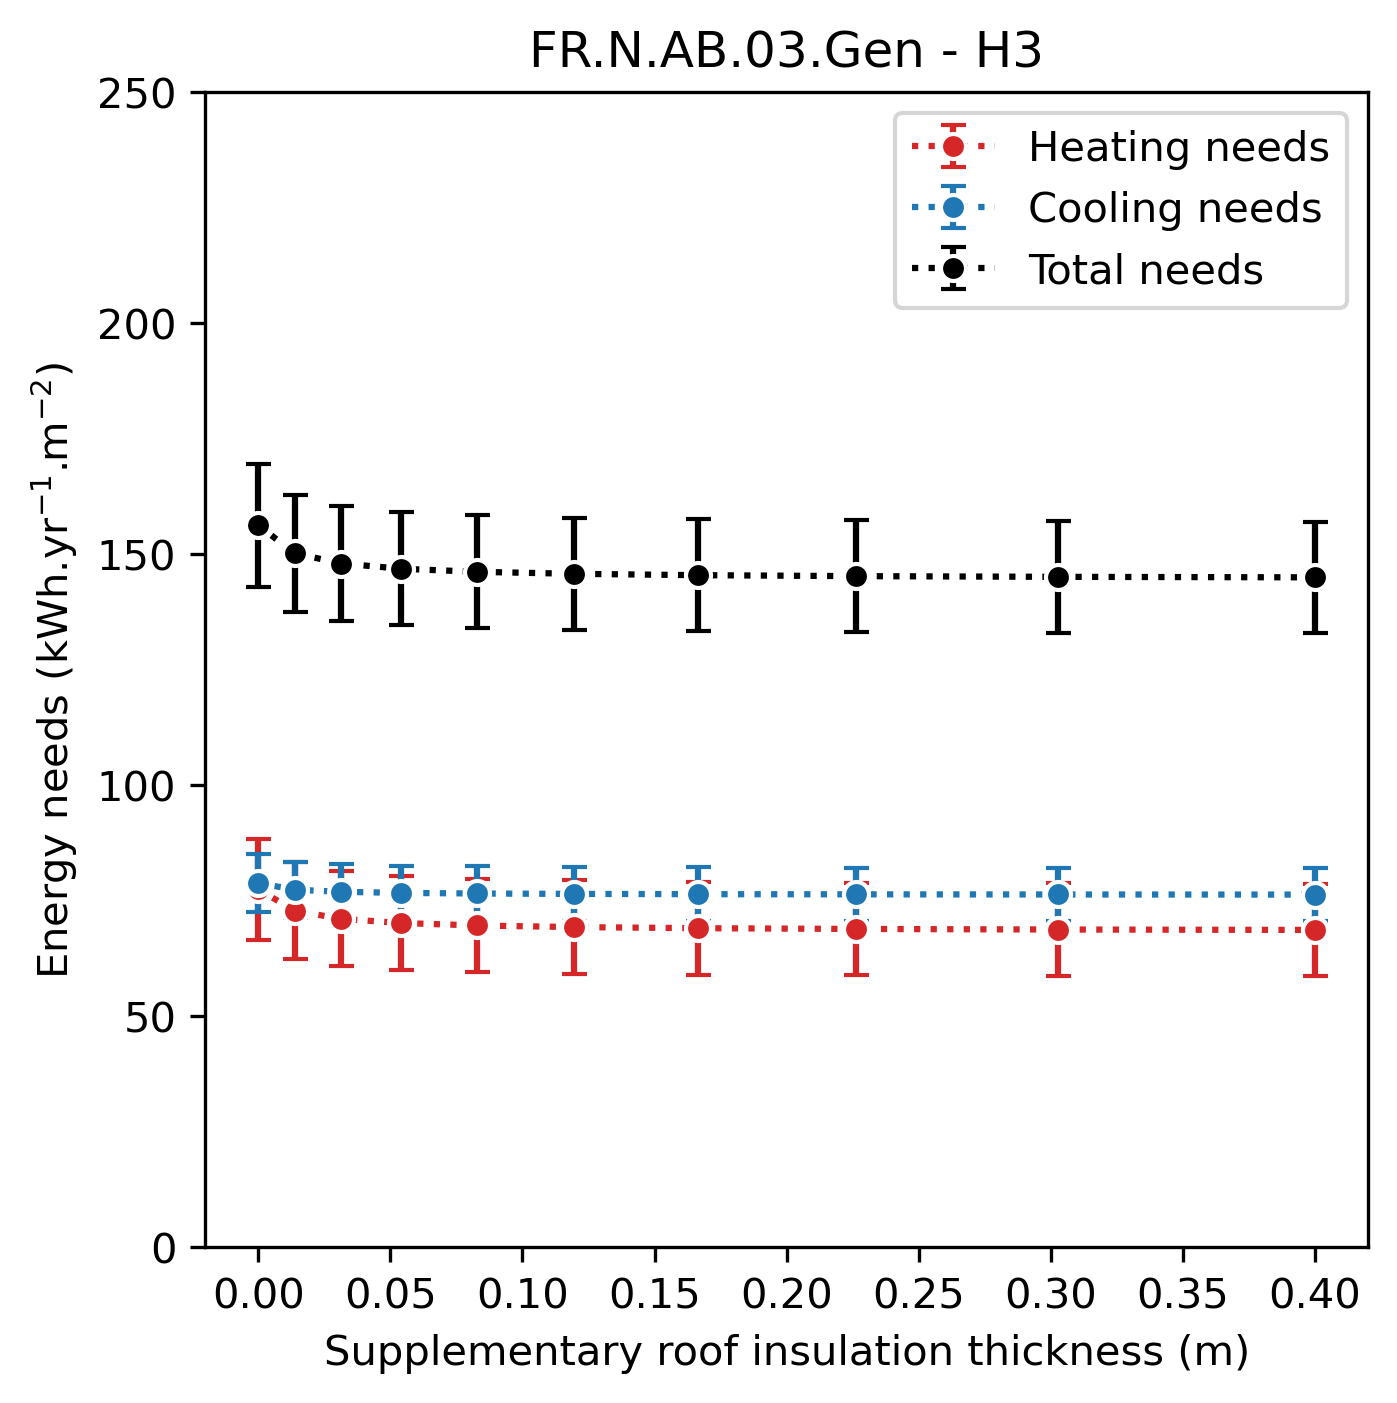
\includegraphics[width=0.32\columnwidth]{figures/roof_FR.N.AB.03.Gen_H3_conventionnel_th-bce_2020_2000-2020.png}
                \caption{\label{fig:roof_init} Effects of roof insulation thickness on energy needs.}
                \begin{quote}
                    \vspace{-2mm}
                    \small\noindent
                    \textbf{(left to right)} Description
                  \end{quote}
            \end{figure}

        % subsubsection roof_insulation (end)

        \subsubsection{Walls insulation} % (fold)
        \label{ssub:walls_insulation}

            description des travaux, ITI car facade ancienne la plupart du temps ? 

            commenter l'interaction (\ref{fig:walls_init})

            \begin{figure}[ht]
                \centering
                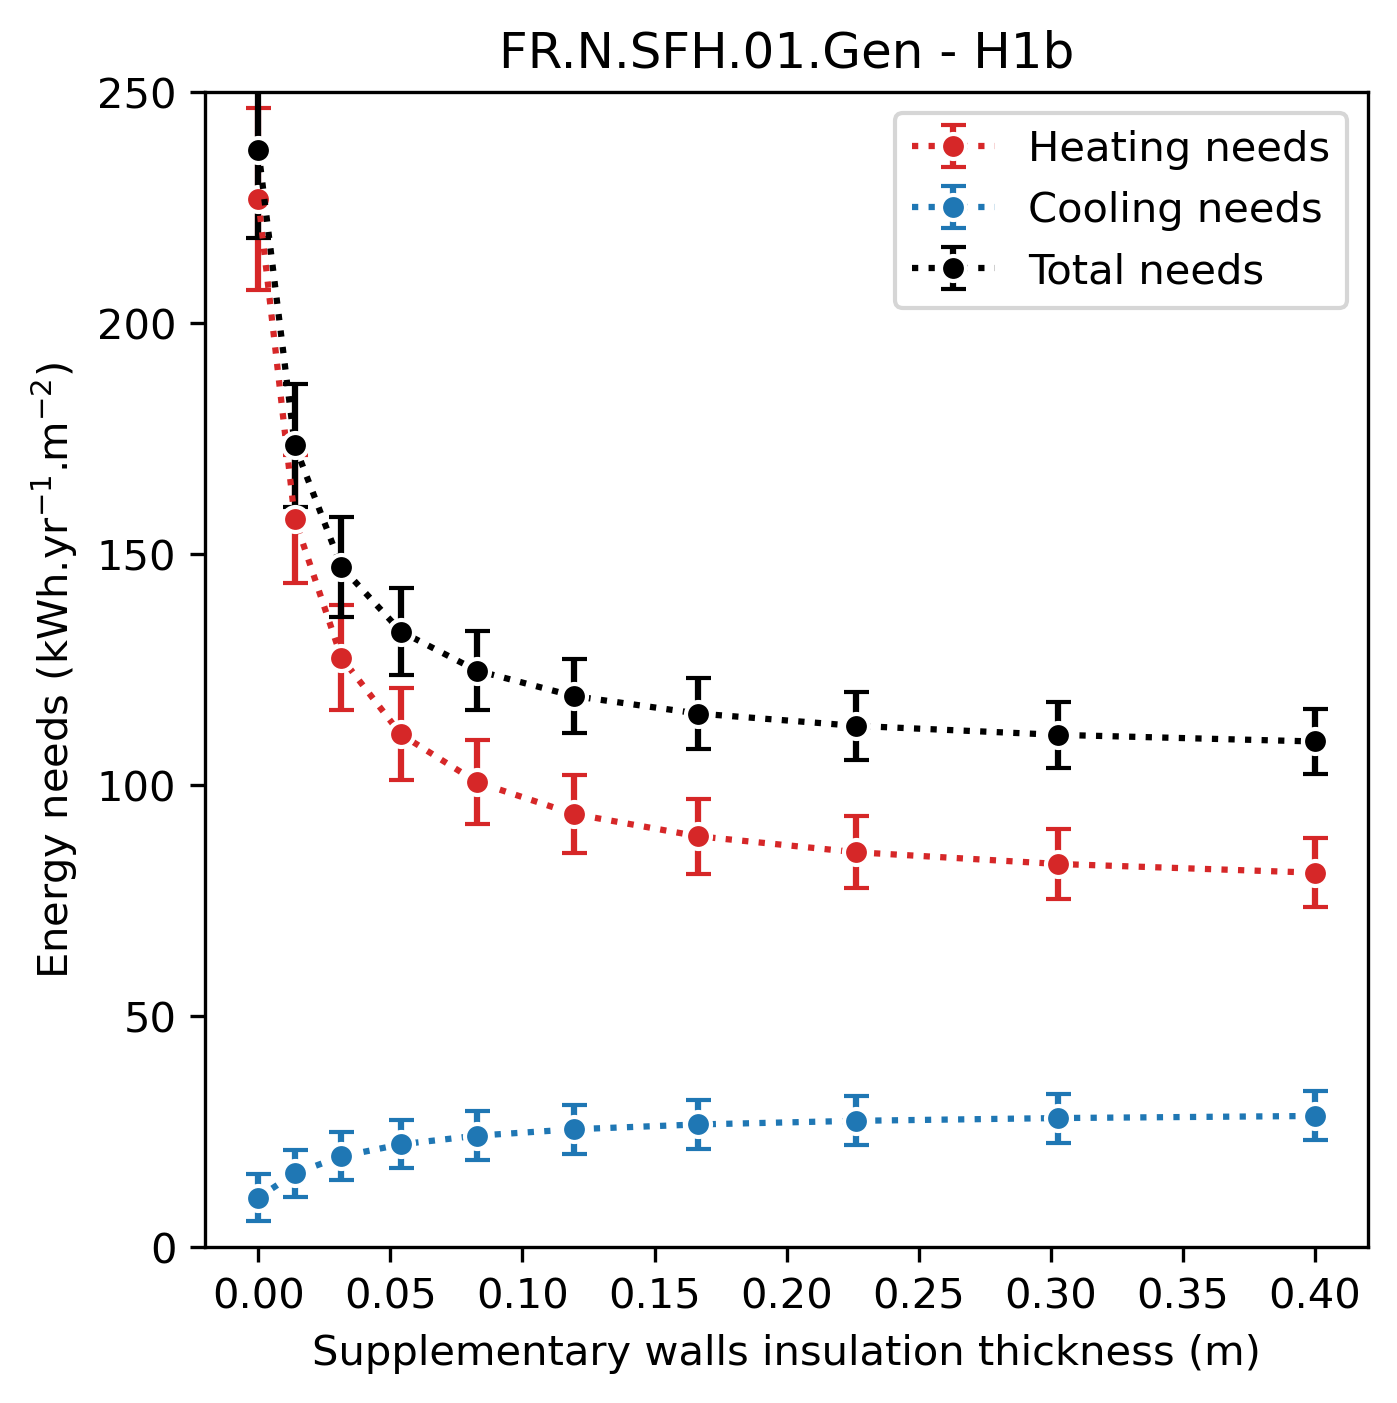
\includegraphics[width=0.32\columnwidth]{figures/walls_FR.N.SFH.01.Gen_H1b_conventionnel_th-bce_2020_2000-2020.png}
                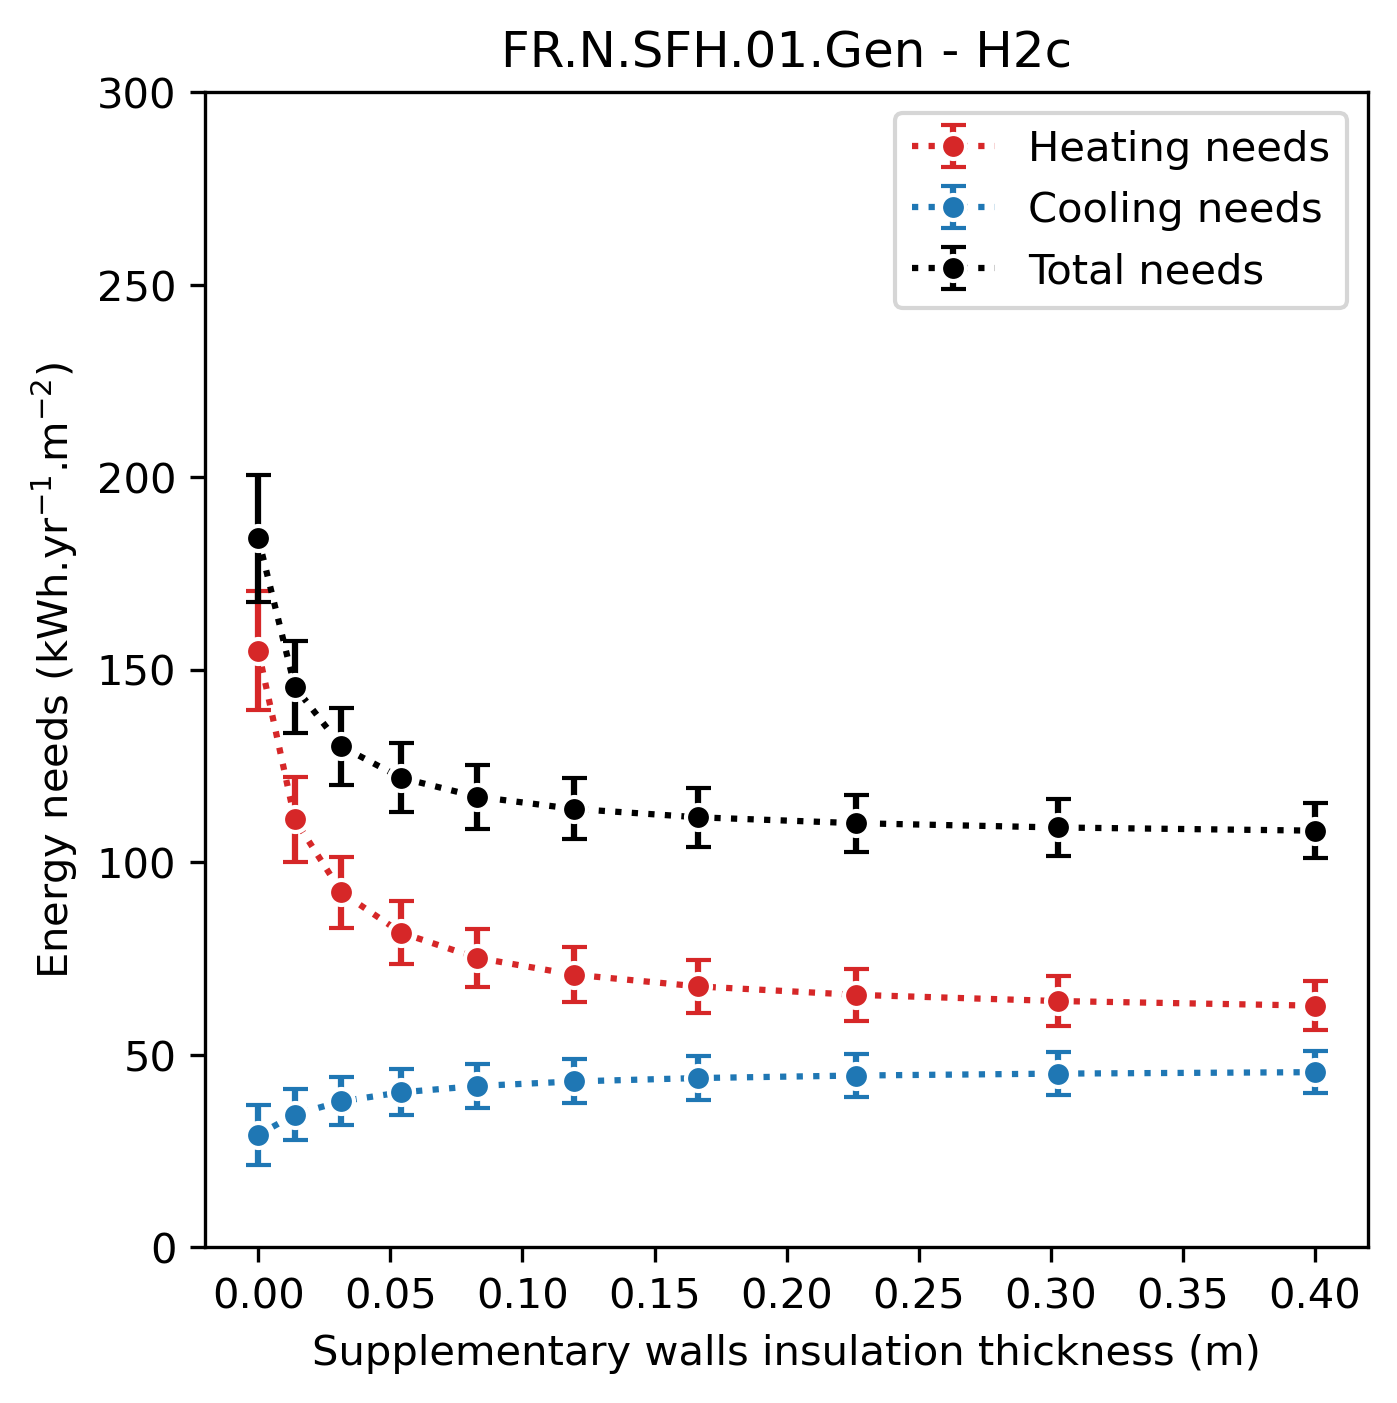
\includegraphics[width=0.32\columnwidth]{figures/walls_FR.N.SFH.01.Gen_H2c_conventionnel_th-bce_2020_2000-2020.png}
                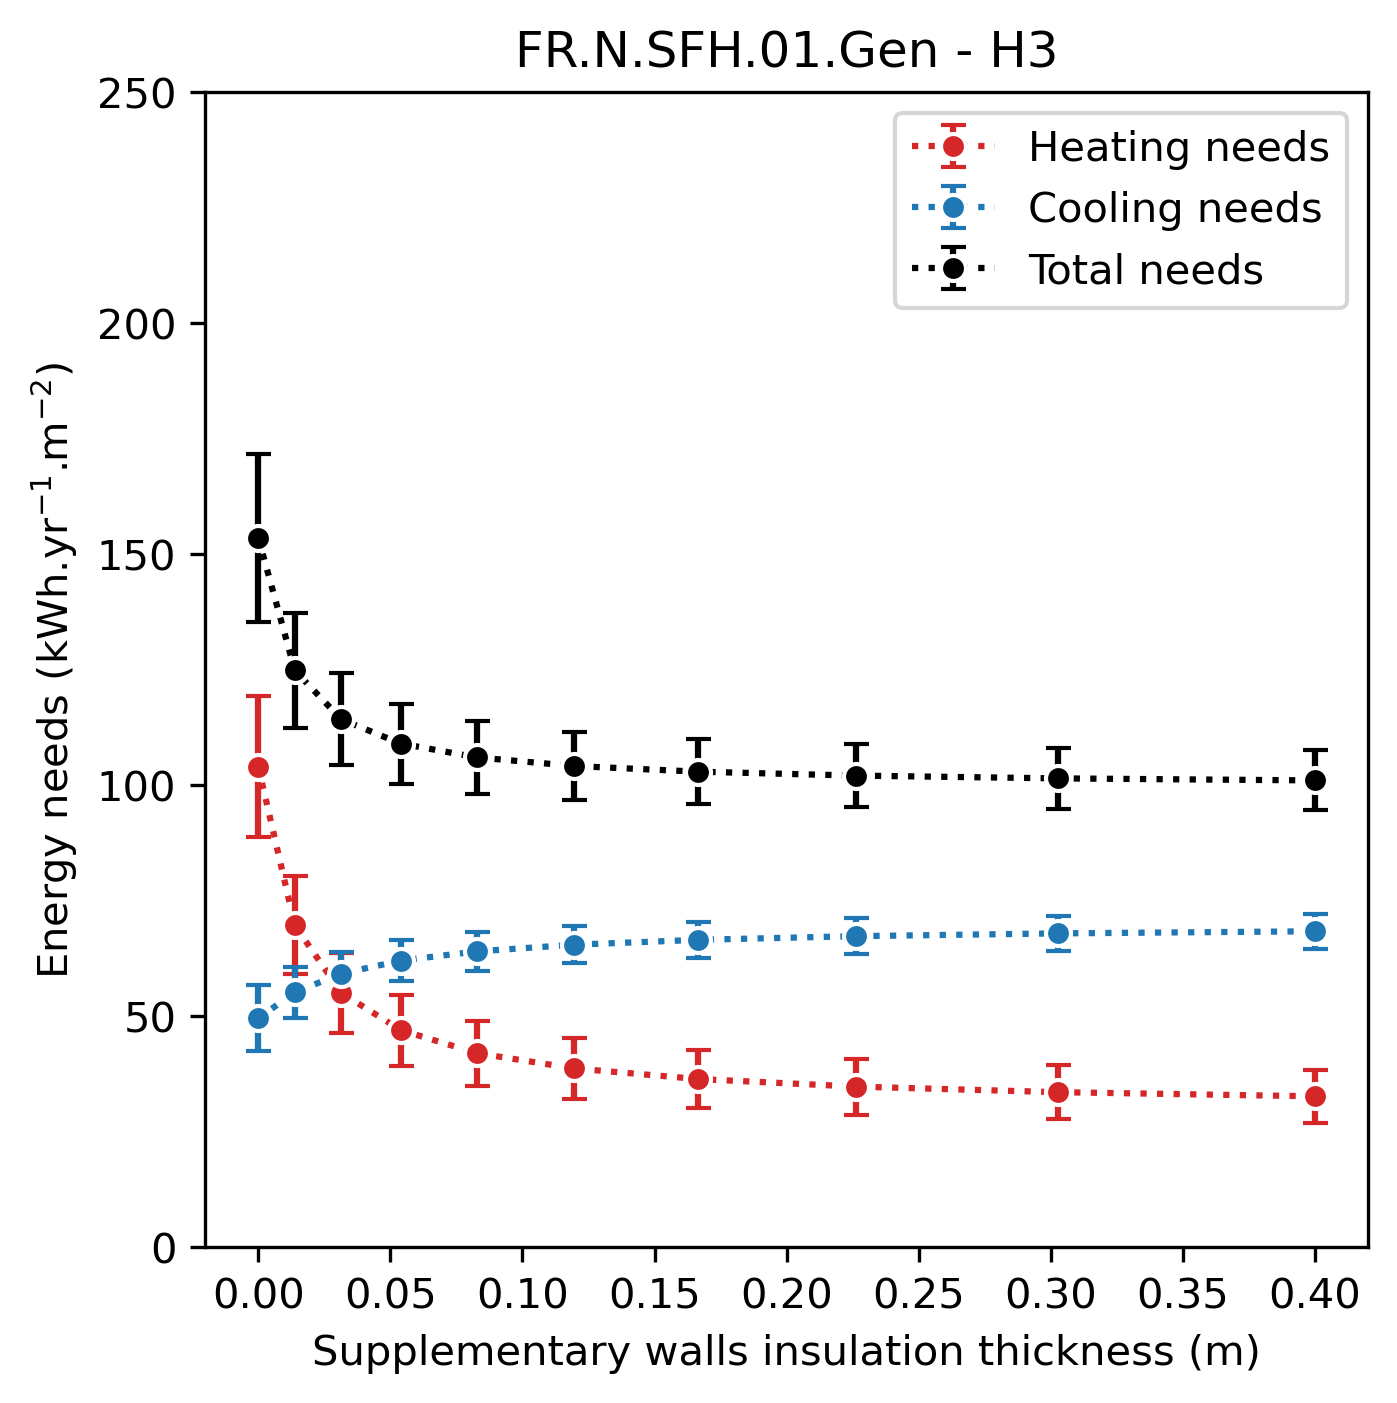
\includegraphics[width=0.32\columnwidth]{figures/walls_FR.N.SFH.01.Gen_H3_conventionnel_th-bce_2020_2000-2020.png}\\
                % 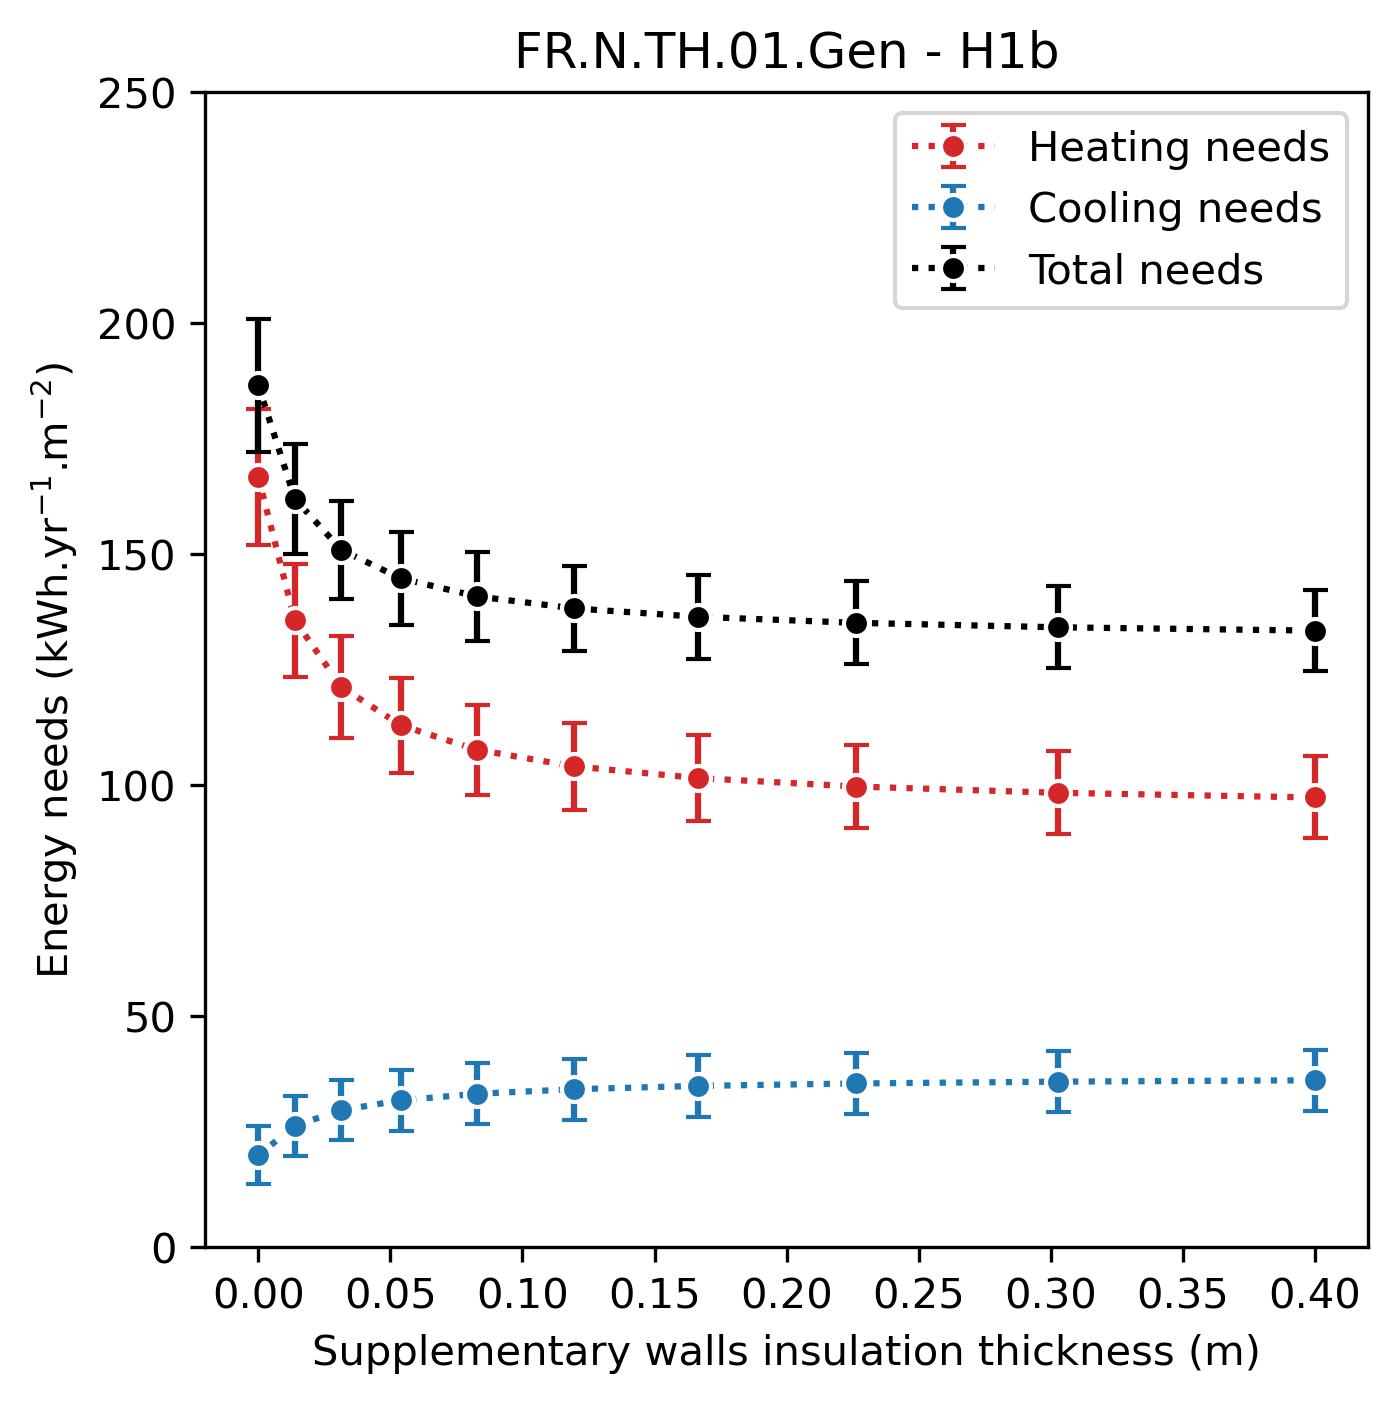
\includegraphics[width=0.32\columnwidth]{figures/walls_FR.N.TH.01.Gen_H1b_conventionnel_th-bce_2020_2000-2020.png}
                % 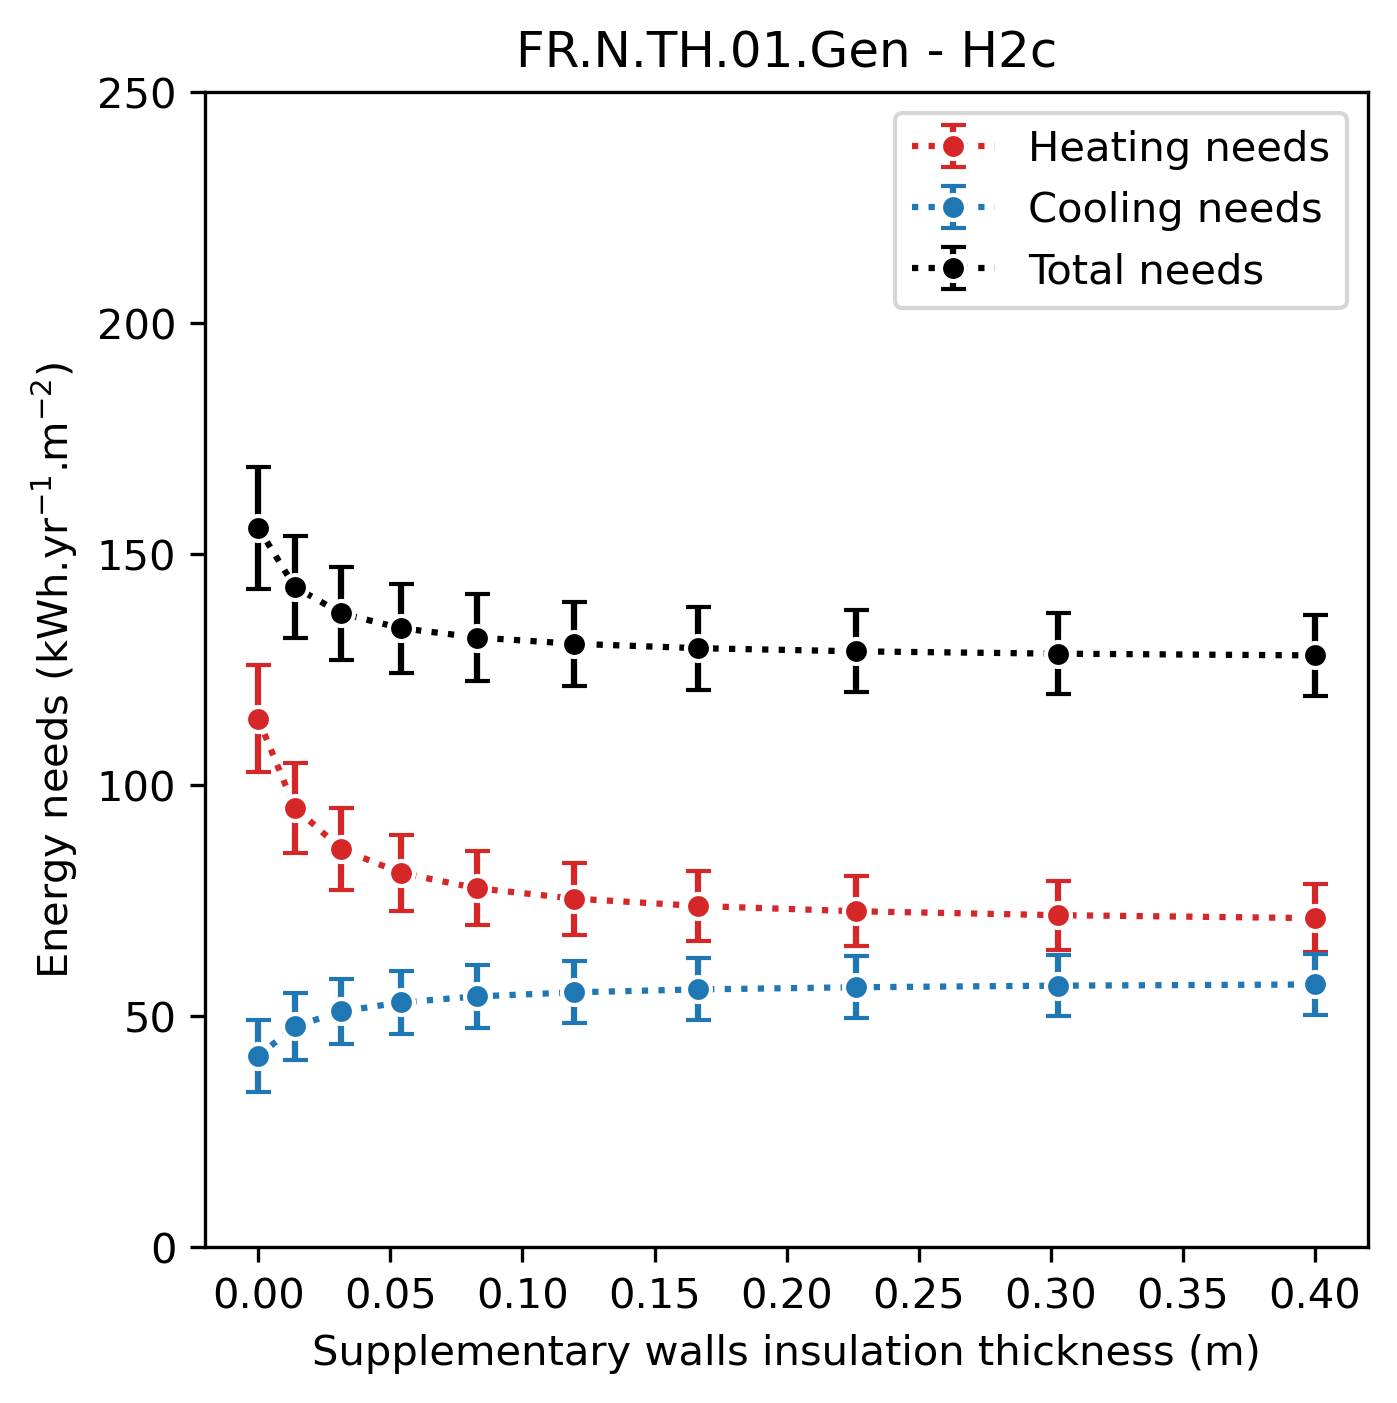
\includegraphics[width=0.32\columnwidth]{figures/walls_FR.N.TH.01.Gen_H2c_conventionnel_th-bce_2020_2000-2020.png}
                % 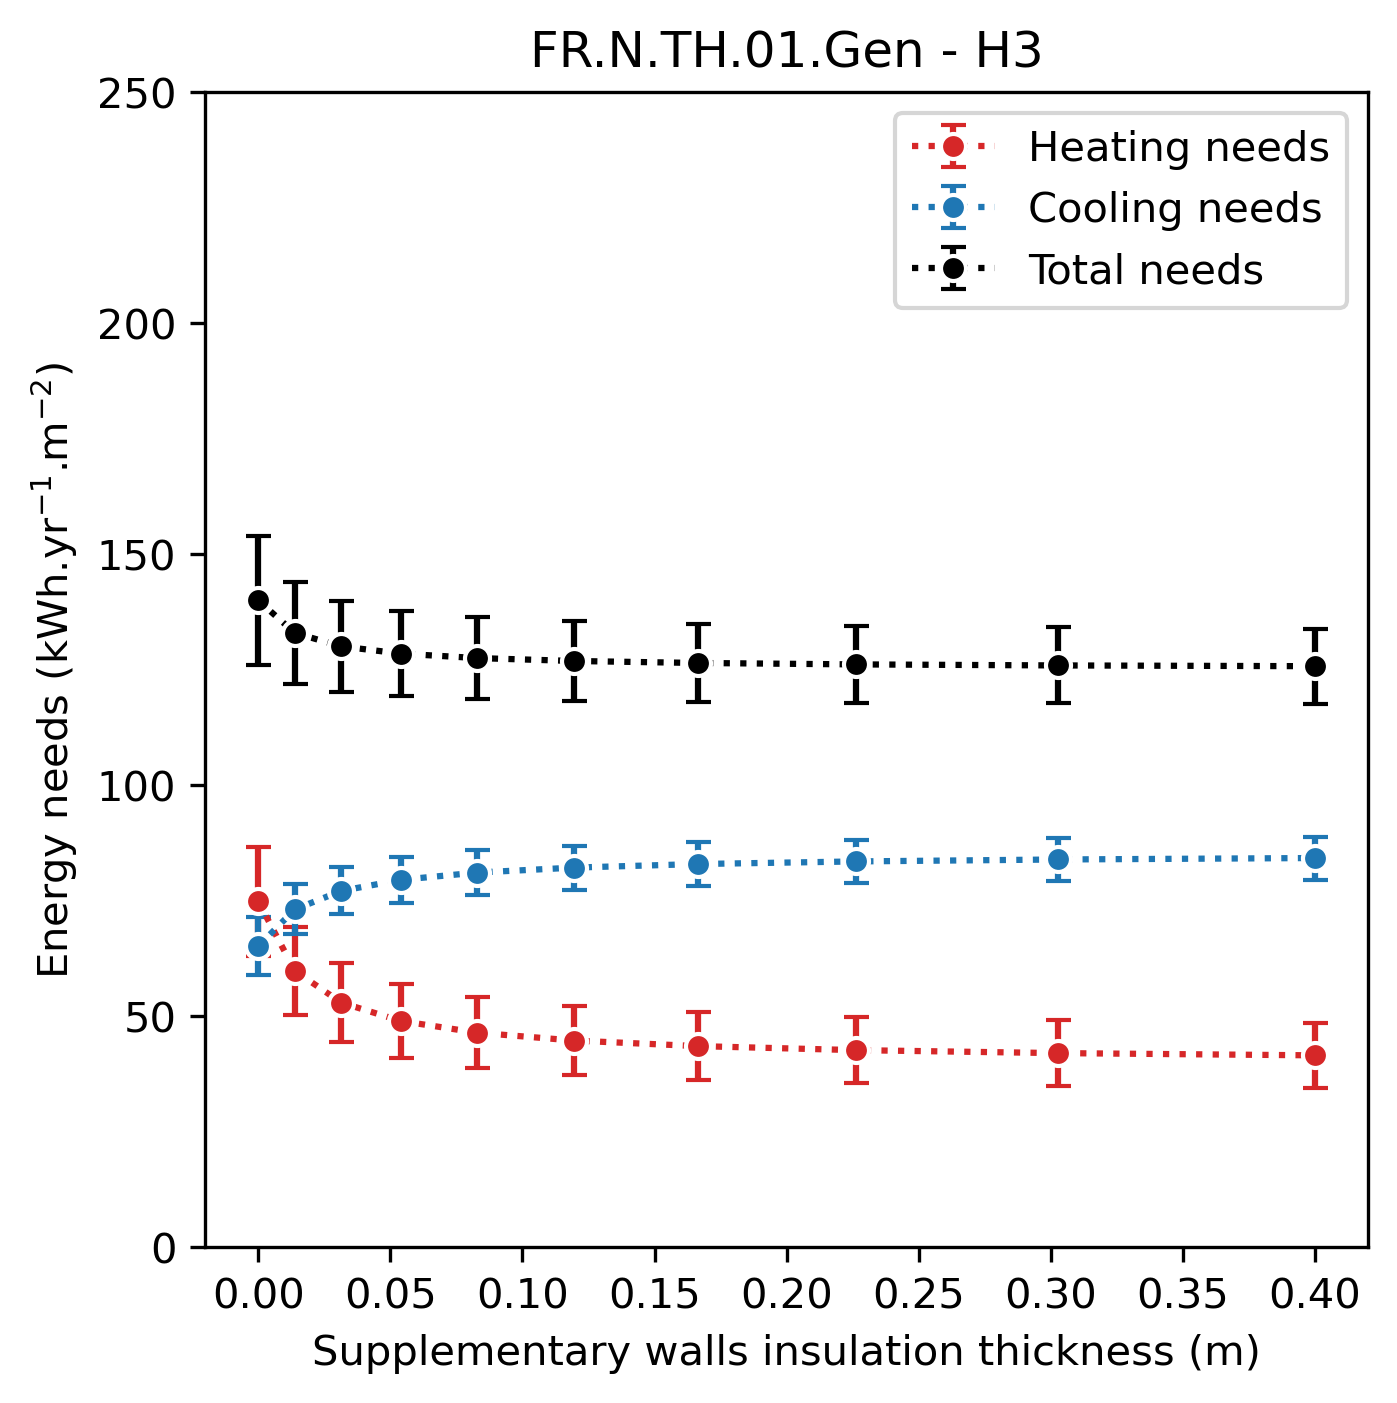
\includegraphics[width=0.32\columnwidth]{figures/walls_FR.N.TH.01.Gen_H3_conventionnel_th-bce_2020_2000-2020.png}\\
                % 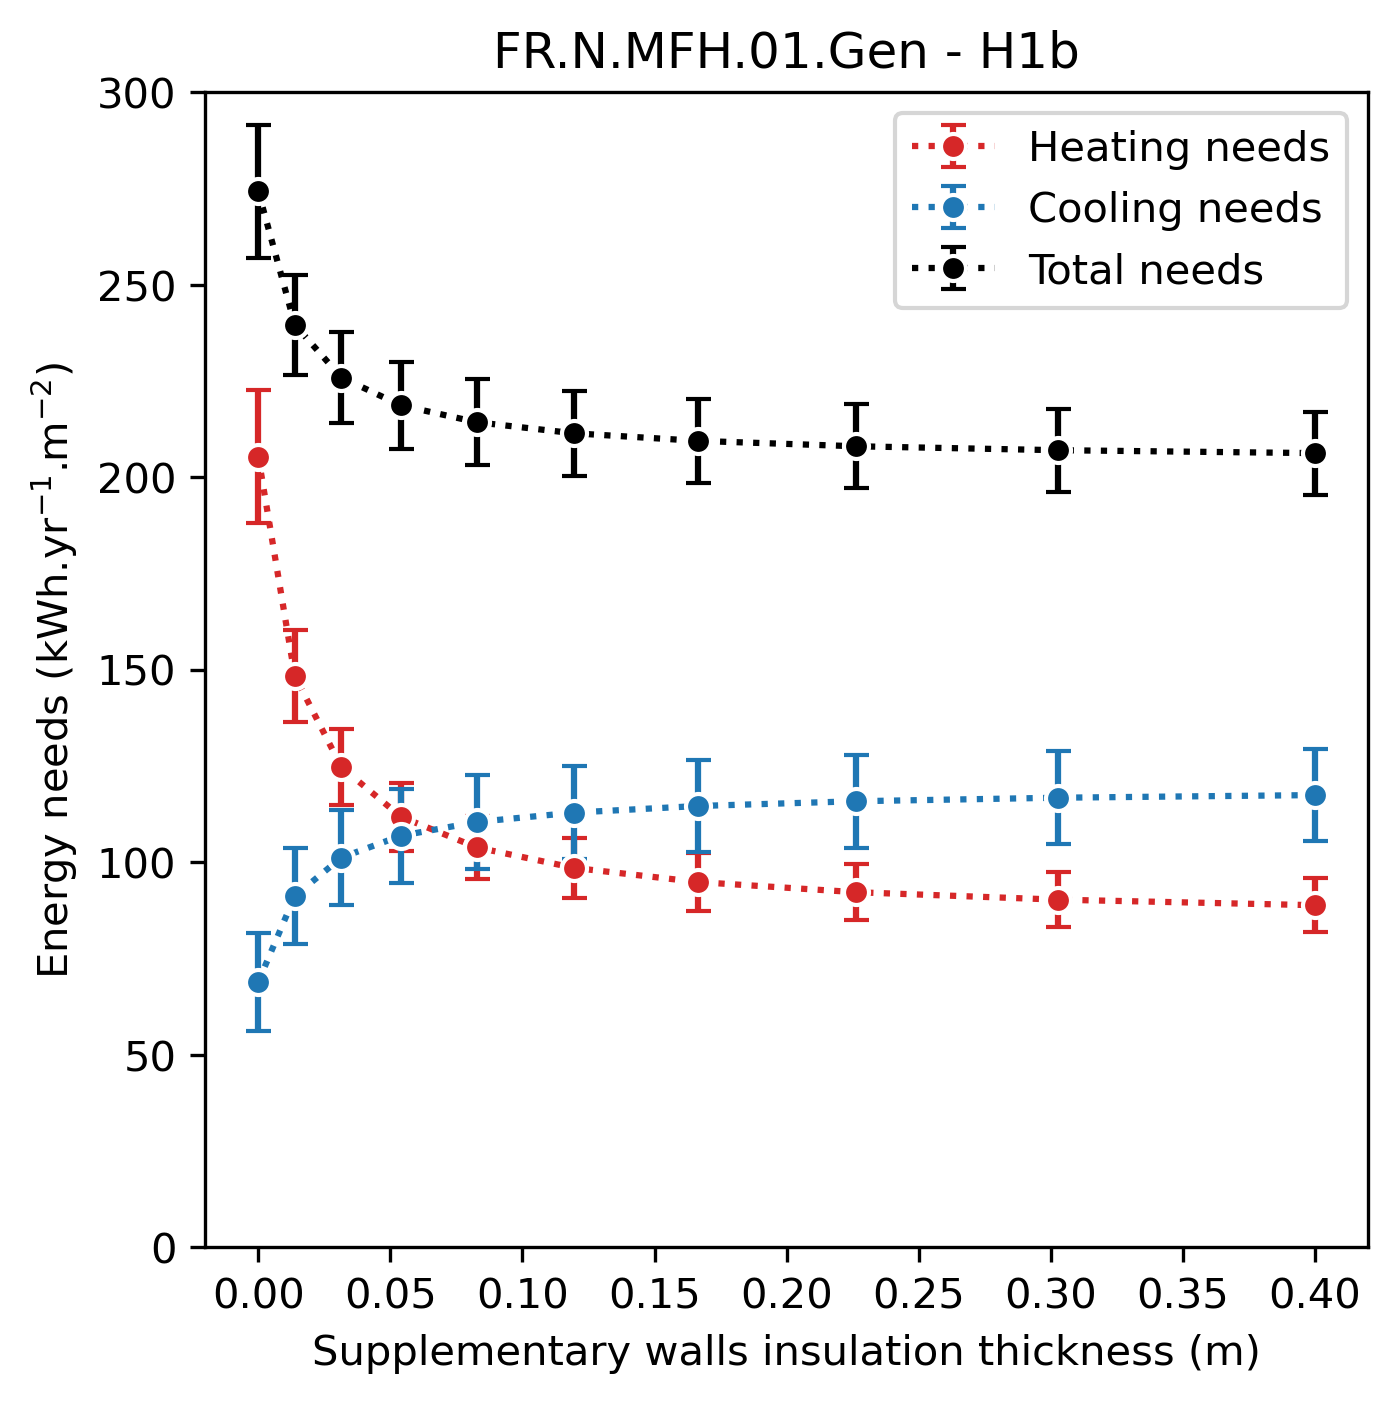
\includegraphics[width=0.32\columnwidth]{figures/walls_FR.N.MFH.01.Gen_H1b_conventionnel_th-bce_2020_2000-2020.png}
                % 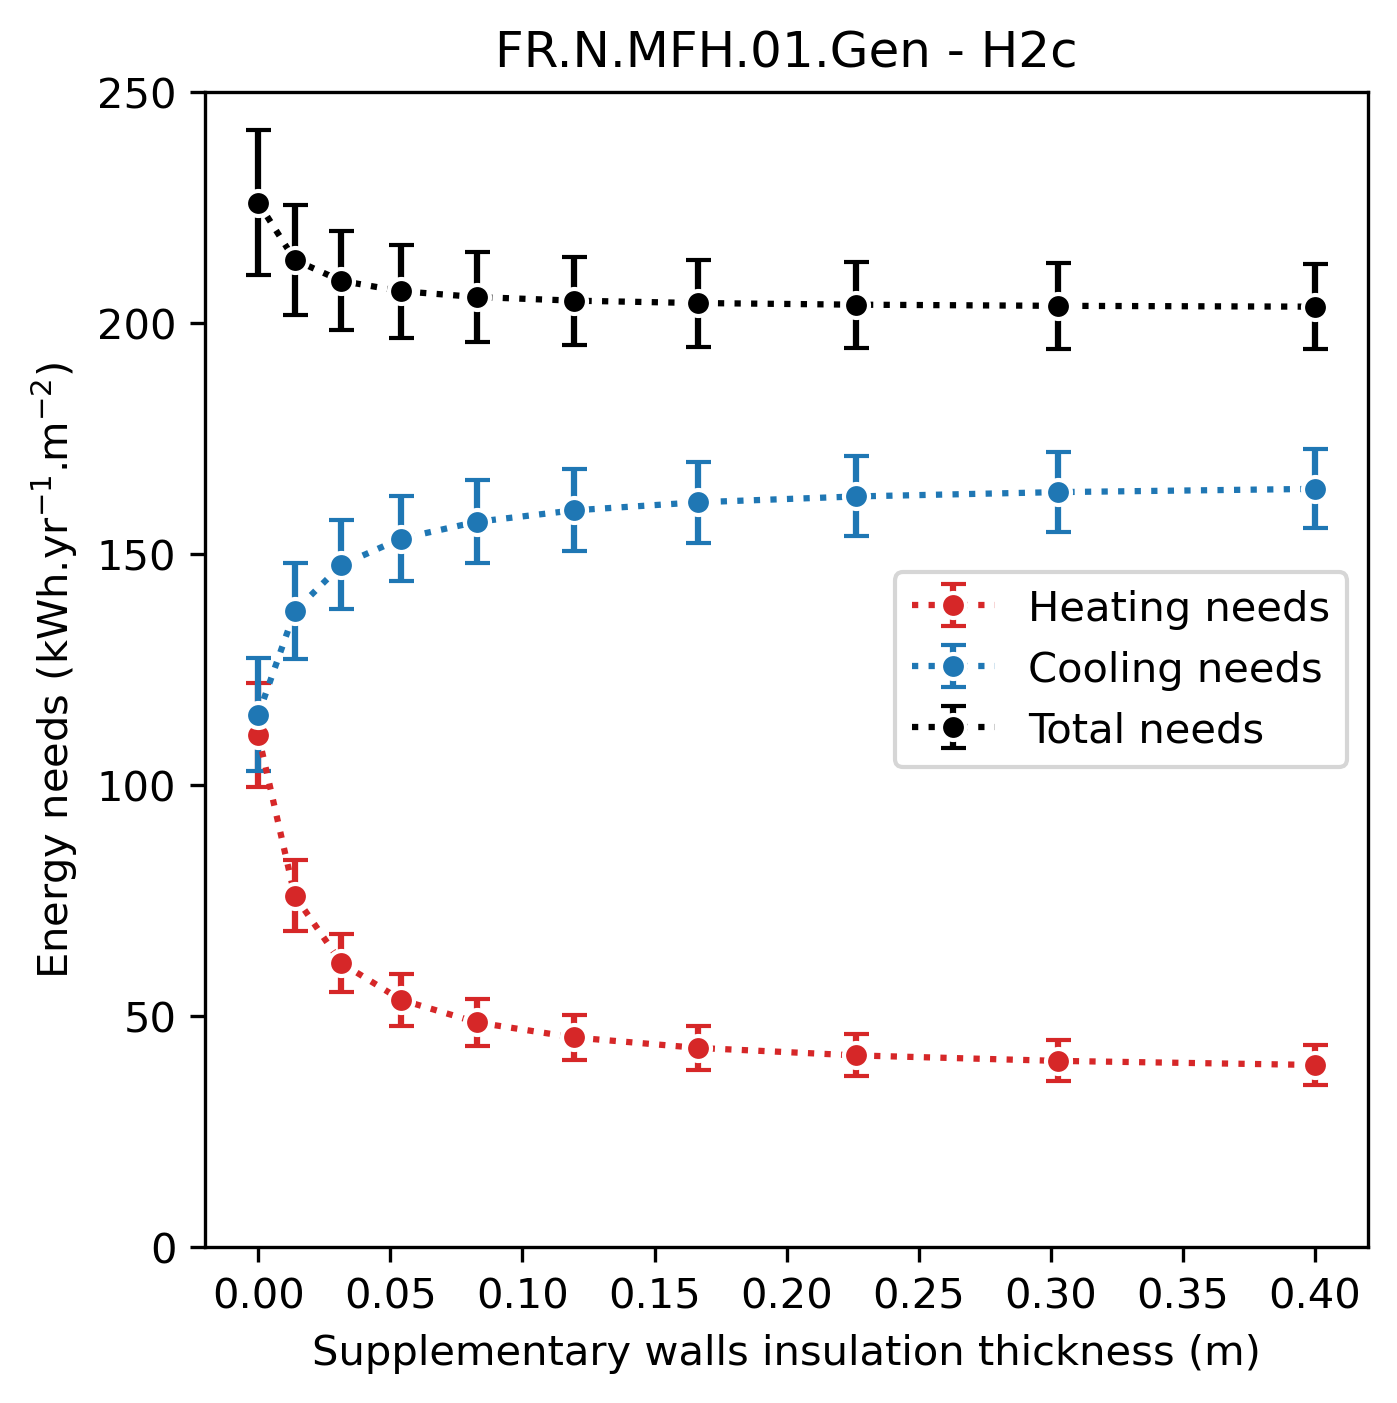
\includegraphics[width=0.32\columnwidth]{figures/walls_FR.N.MFH.01.Gen_H2c_conventionnel_th-bce_2020_2000-2020.png}
                % 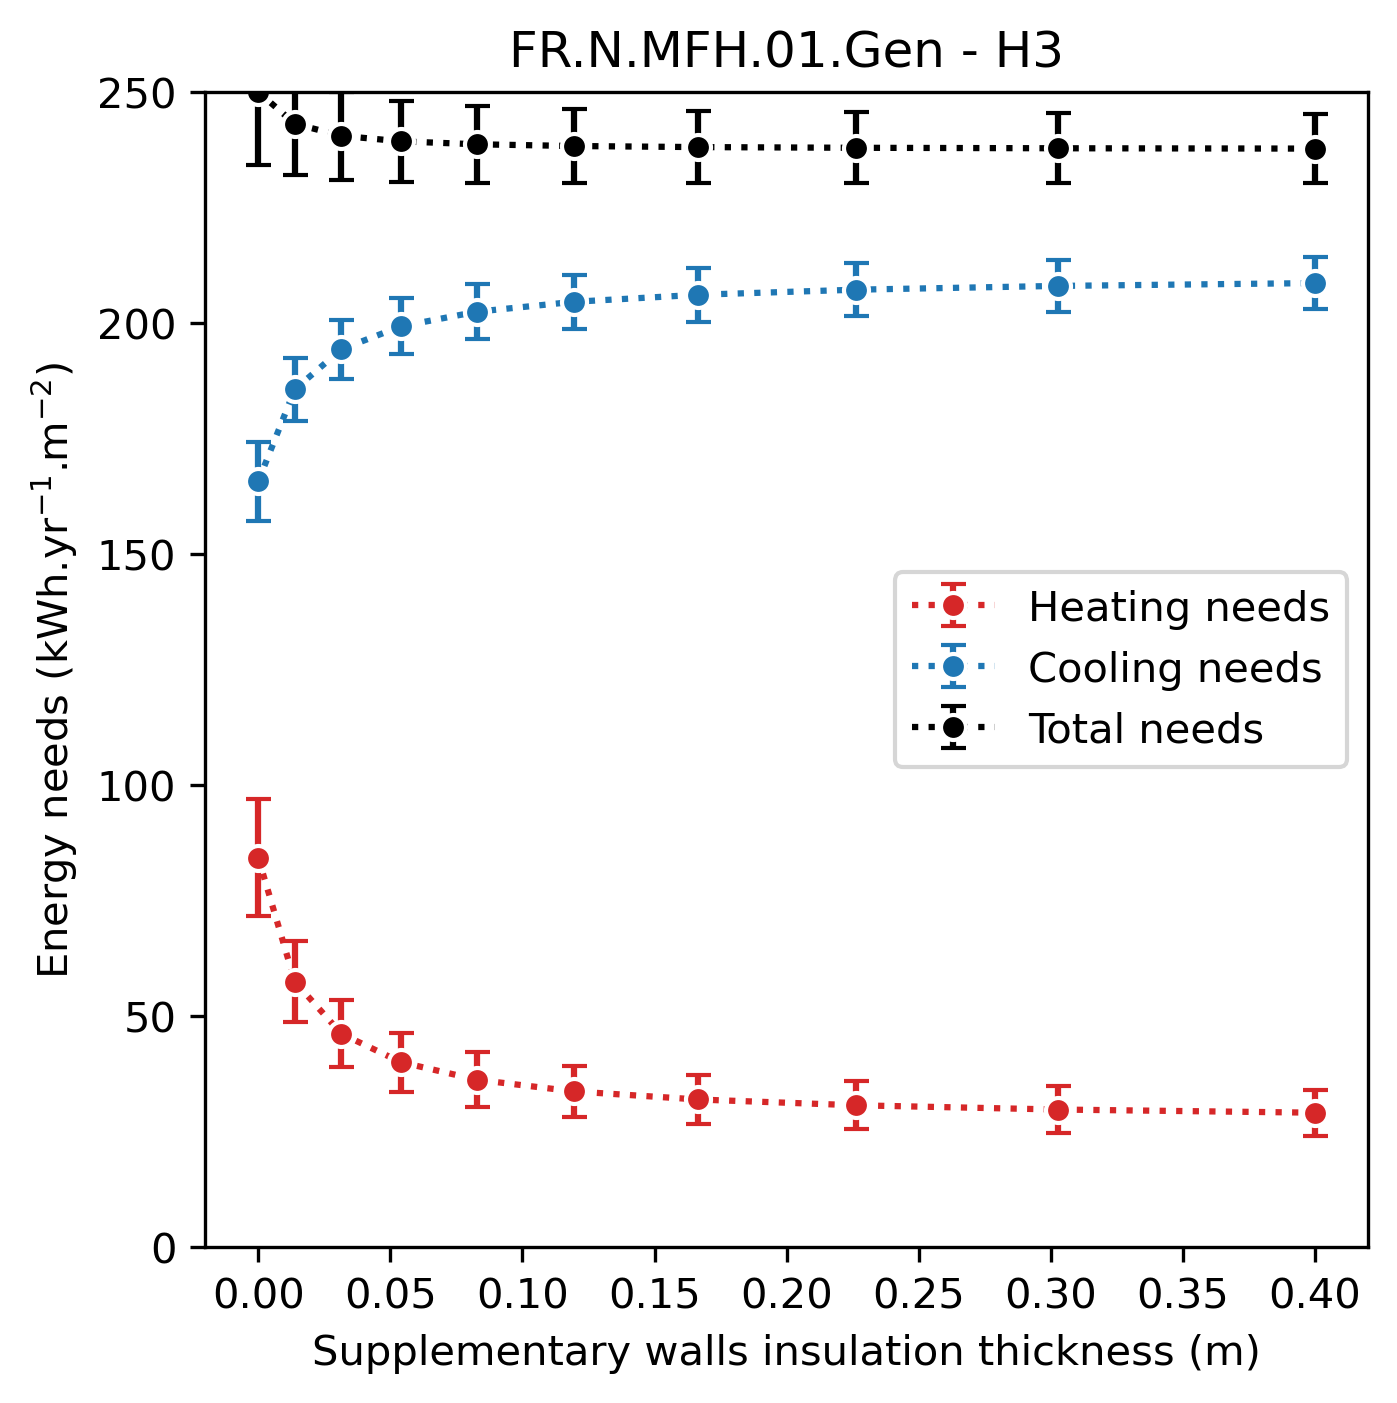
\includegraphics[width=0.32\columnwidth]{figures/walls_FR.N.MFH.01.Gen_H3_conventionnel_th-bce_2020_2000-2020.png}\\
                % 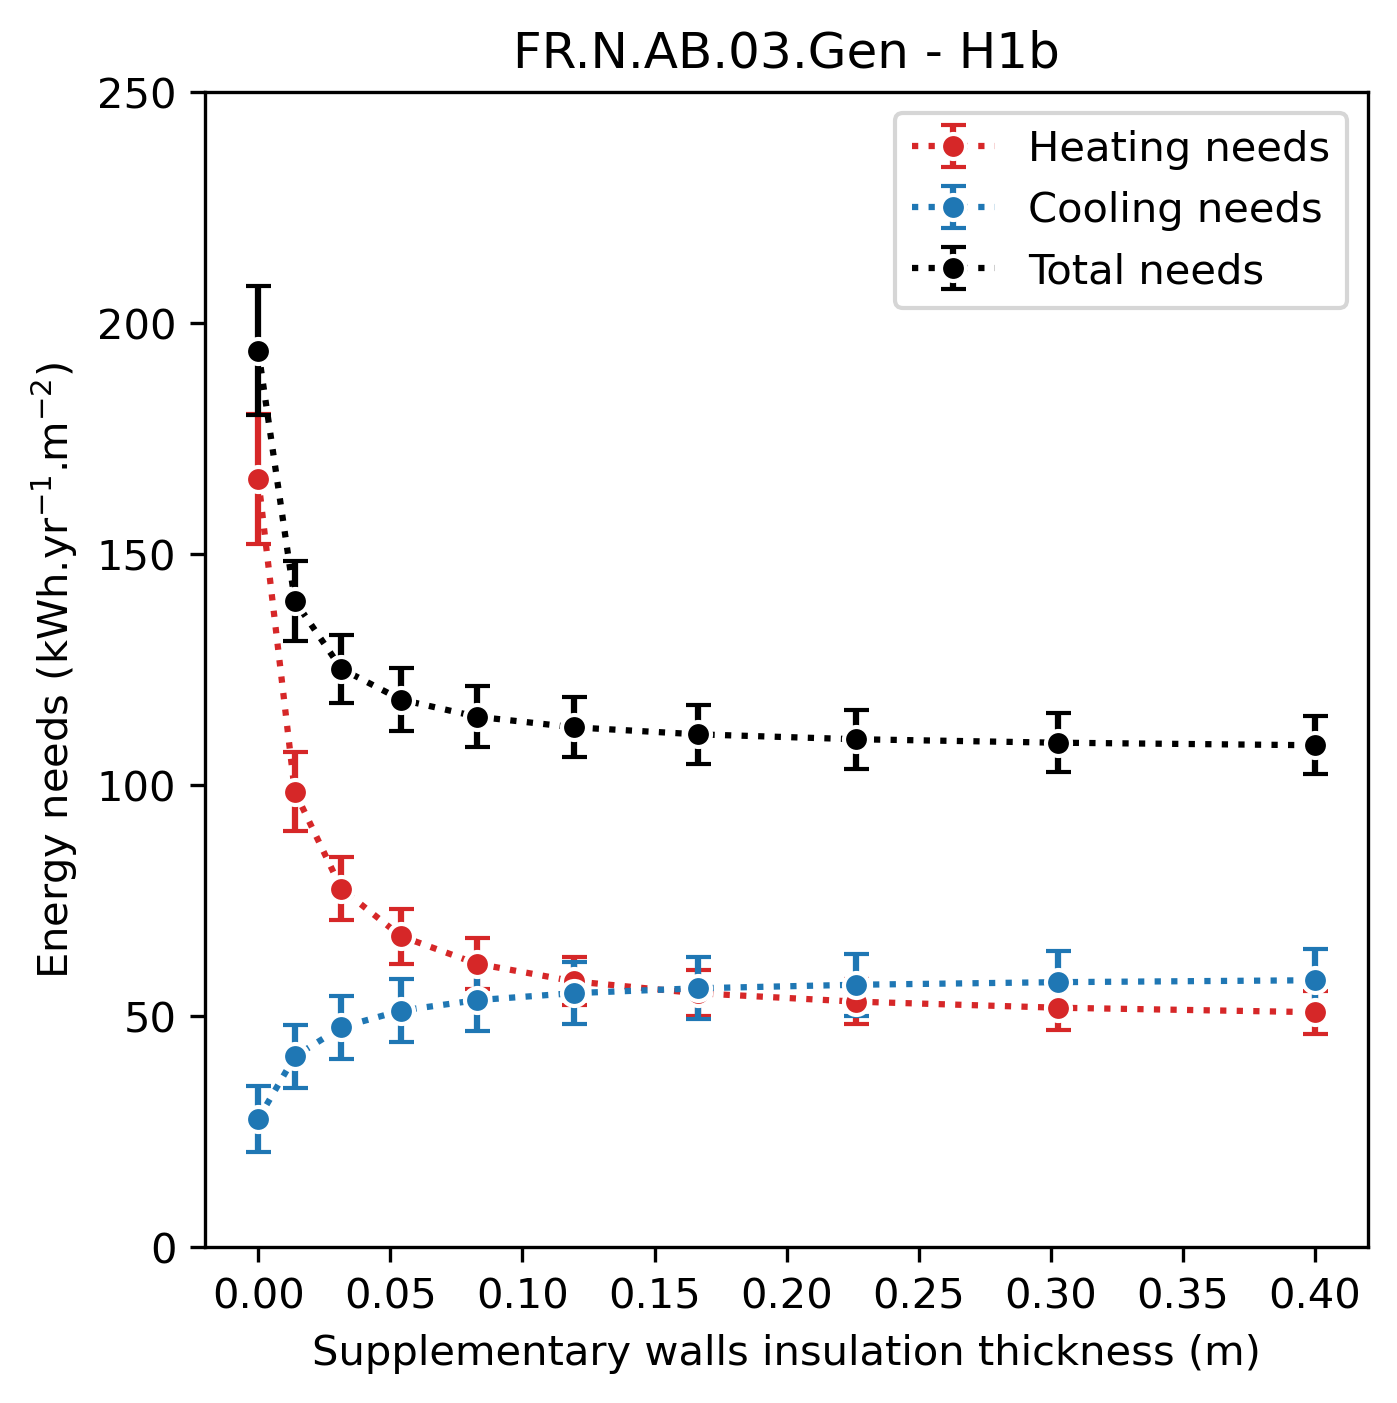
\includegraphics[width=0.32\columnwidth]{figures/walls_FR.N.AB.03.Gen_H1b_conventionnel_th-bce_2020_2000-2020.png}
                % 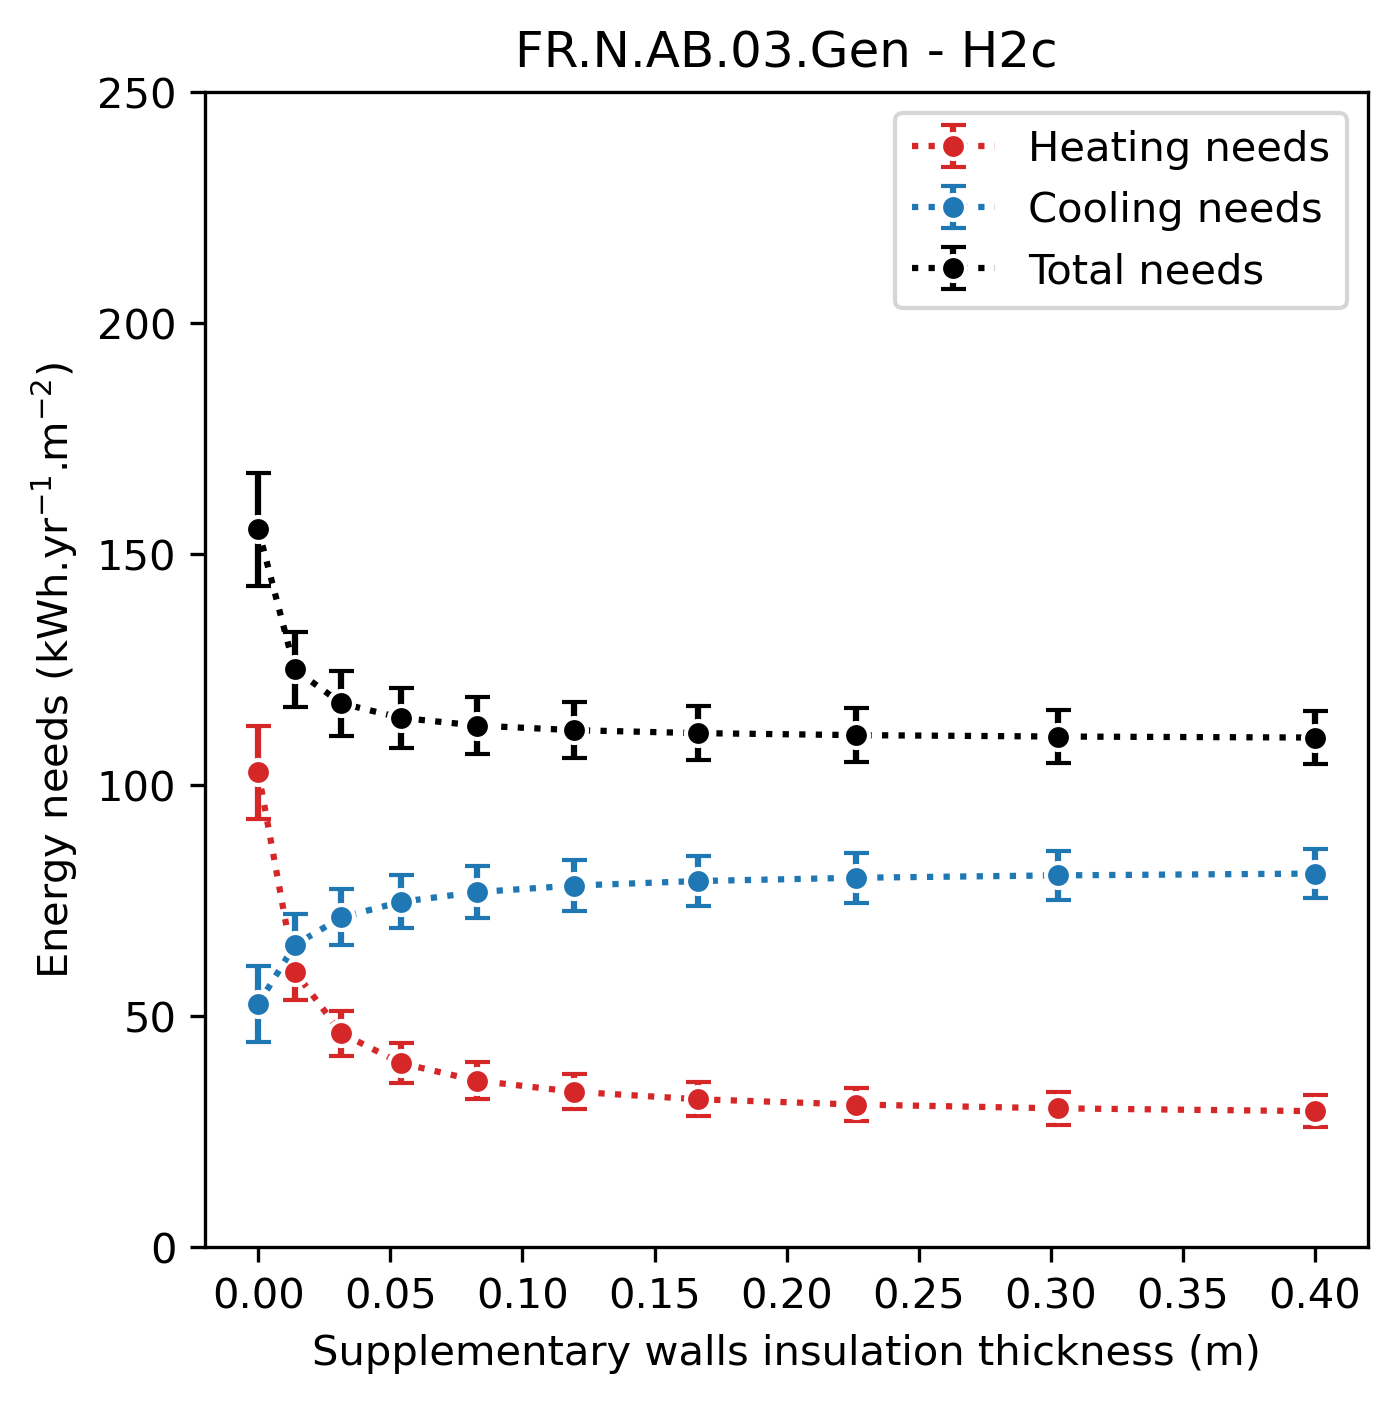
\includegraphics[width=0.32\columnwidth]{figures/walls_FR.N.AB.03.Gen_H2c_conventionnel_th-bce_2020_2000-2020.png}
                % 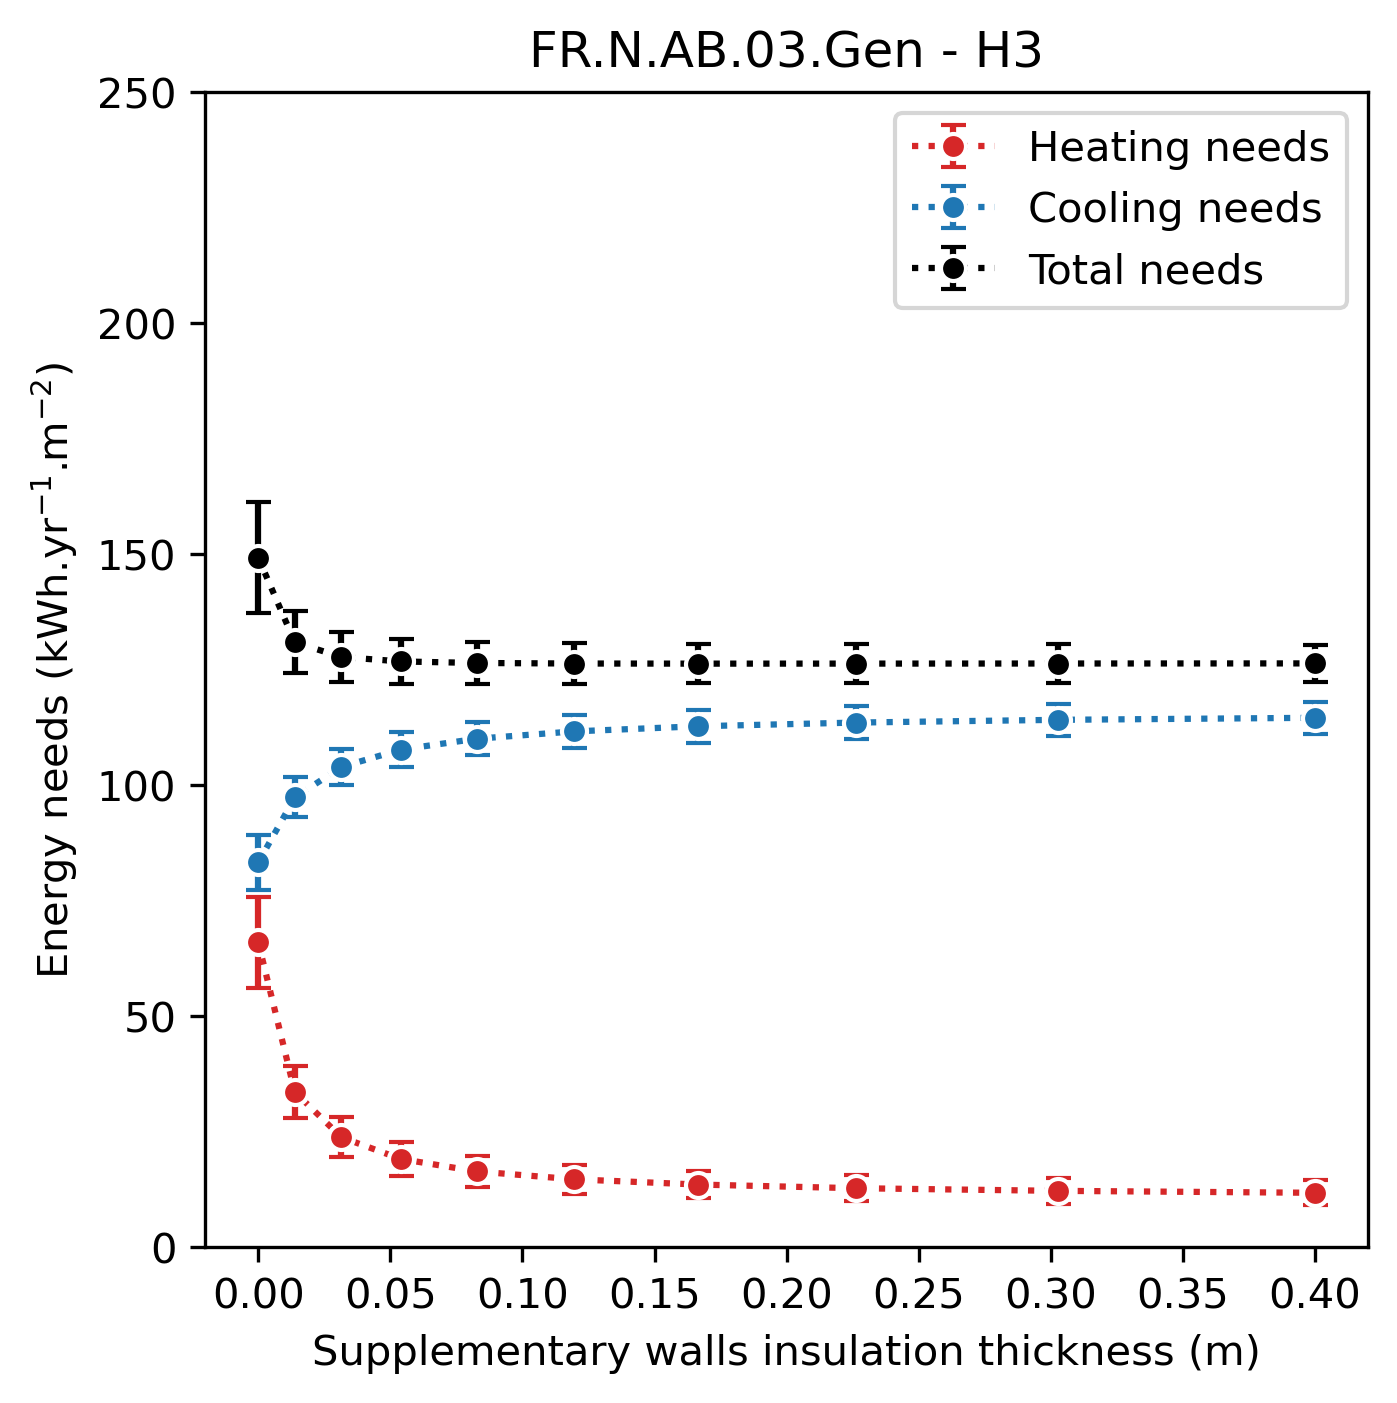
\includegraphics[width=0.32\columnwidth]{figures/walls_FR.N.AB.03.Gen_H3_conventionnel_th-bce_2020_2000-2020.png}
                \caption{\label{fig:walls_init} Effects of walls insulation thickness on energy needs.}
                \begin{quote}
                    \vspace{-2mm}
                    \small\noindent
                    \textbf{(left to right)} Description
                  \end{quote}
            \end{figure}
        
        % subsubsection walls_insulation (end)

        \subsubsection{Floor insulation} % (fold)
        \label{ssub:floor_insulation}

        description des travaux etc.

        detailler les interactions (\ref{fig:floor_init})

        detailler le cas des batiments collectifs 

            \begin{figure}[ht]
                \centering
                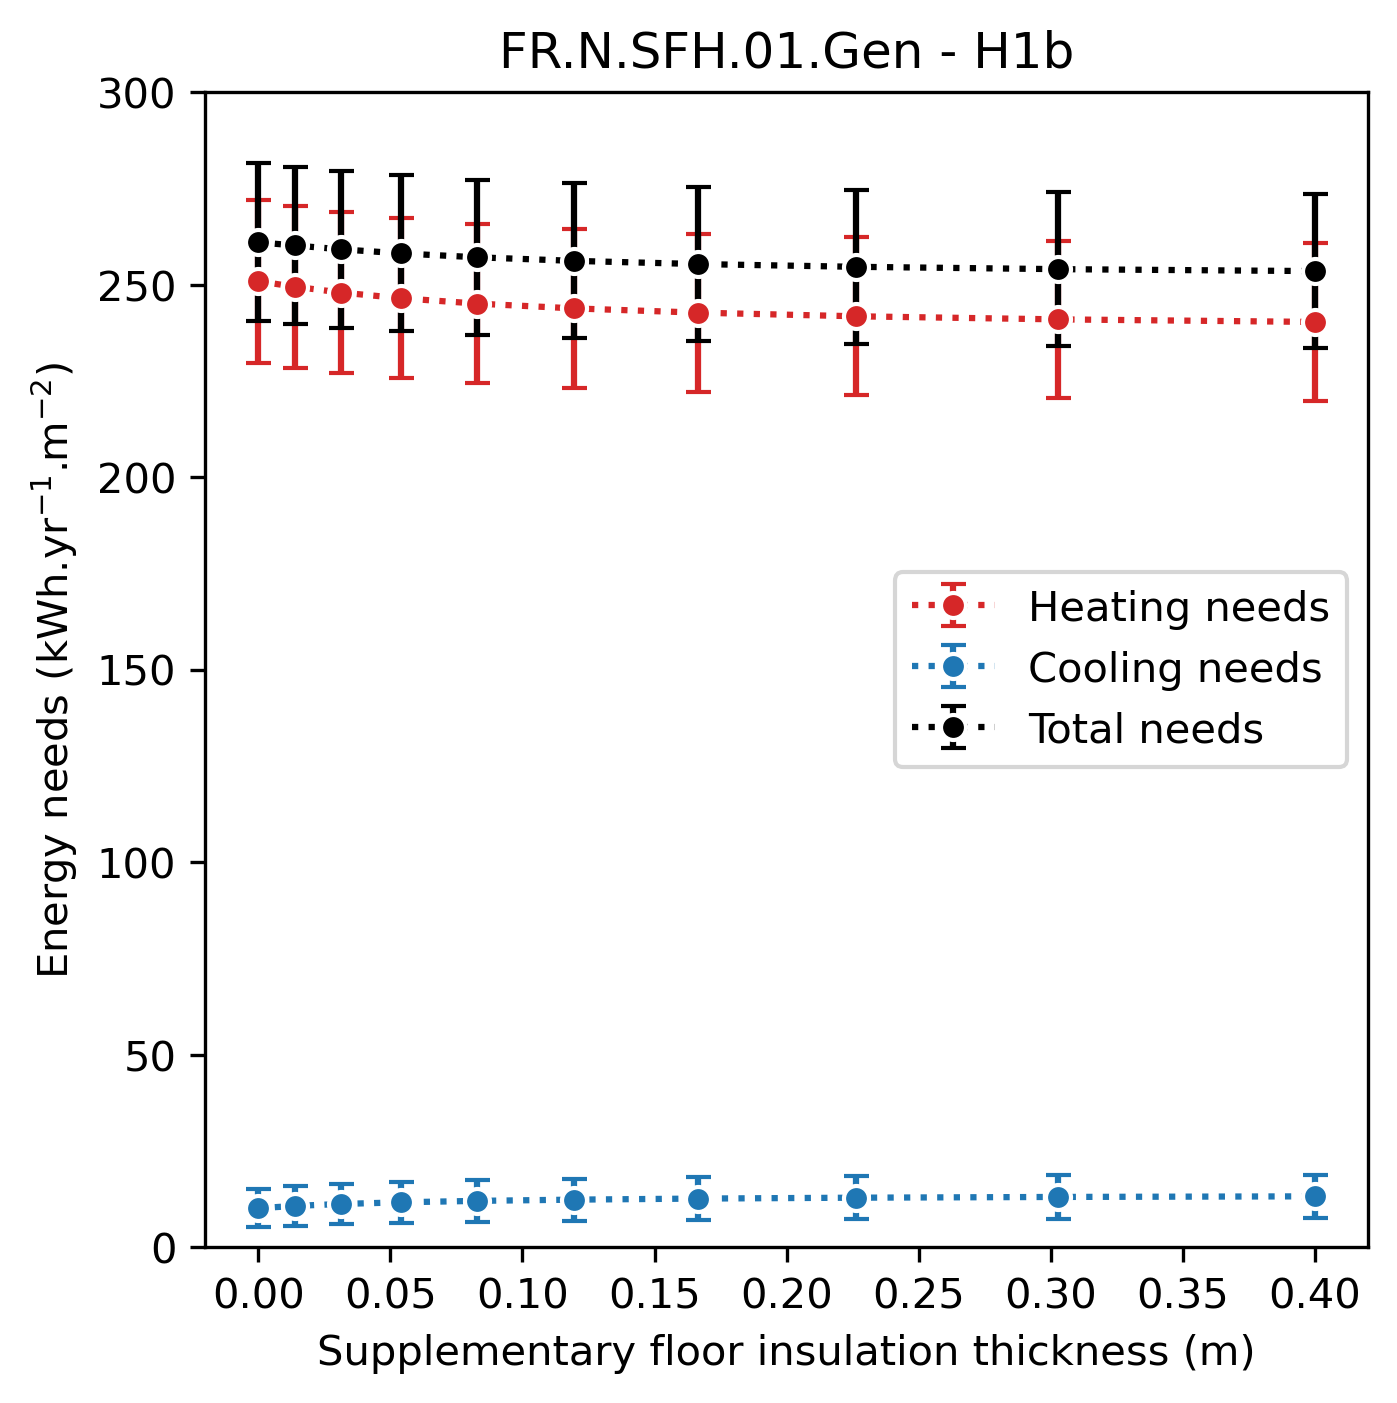
\includegraphics[width=0.32\columnwidth]{figures/floor_FR.N.SFH.01.Gen_H1b_conventionnel_th-bce_2020_2000-2020.png}
                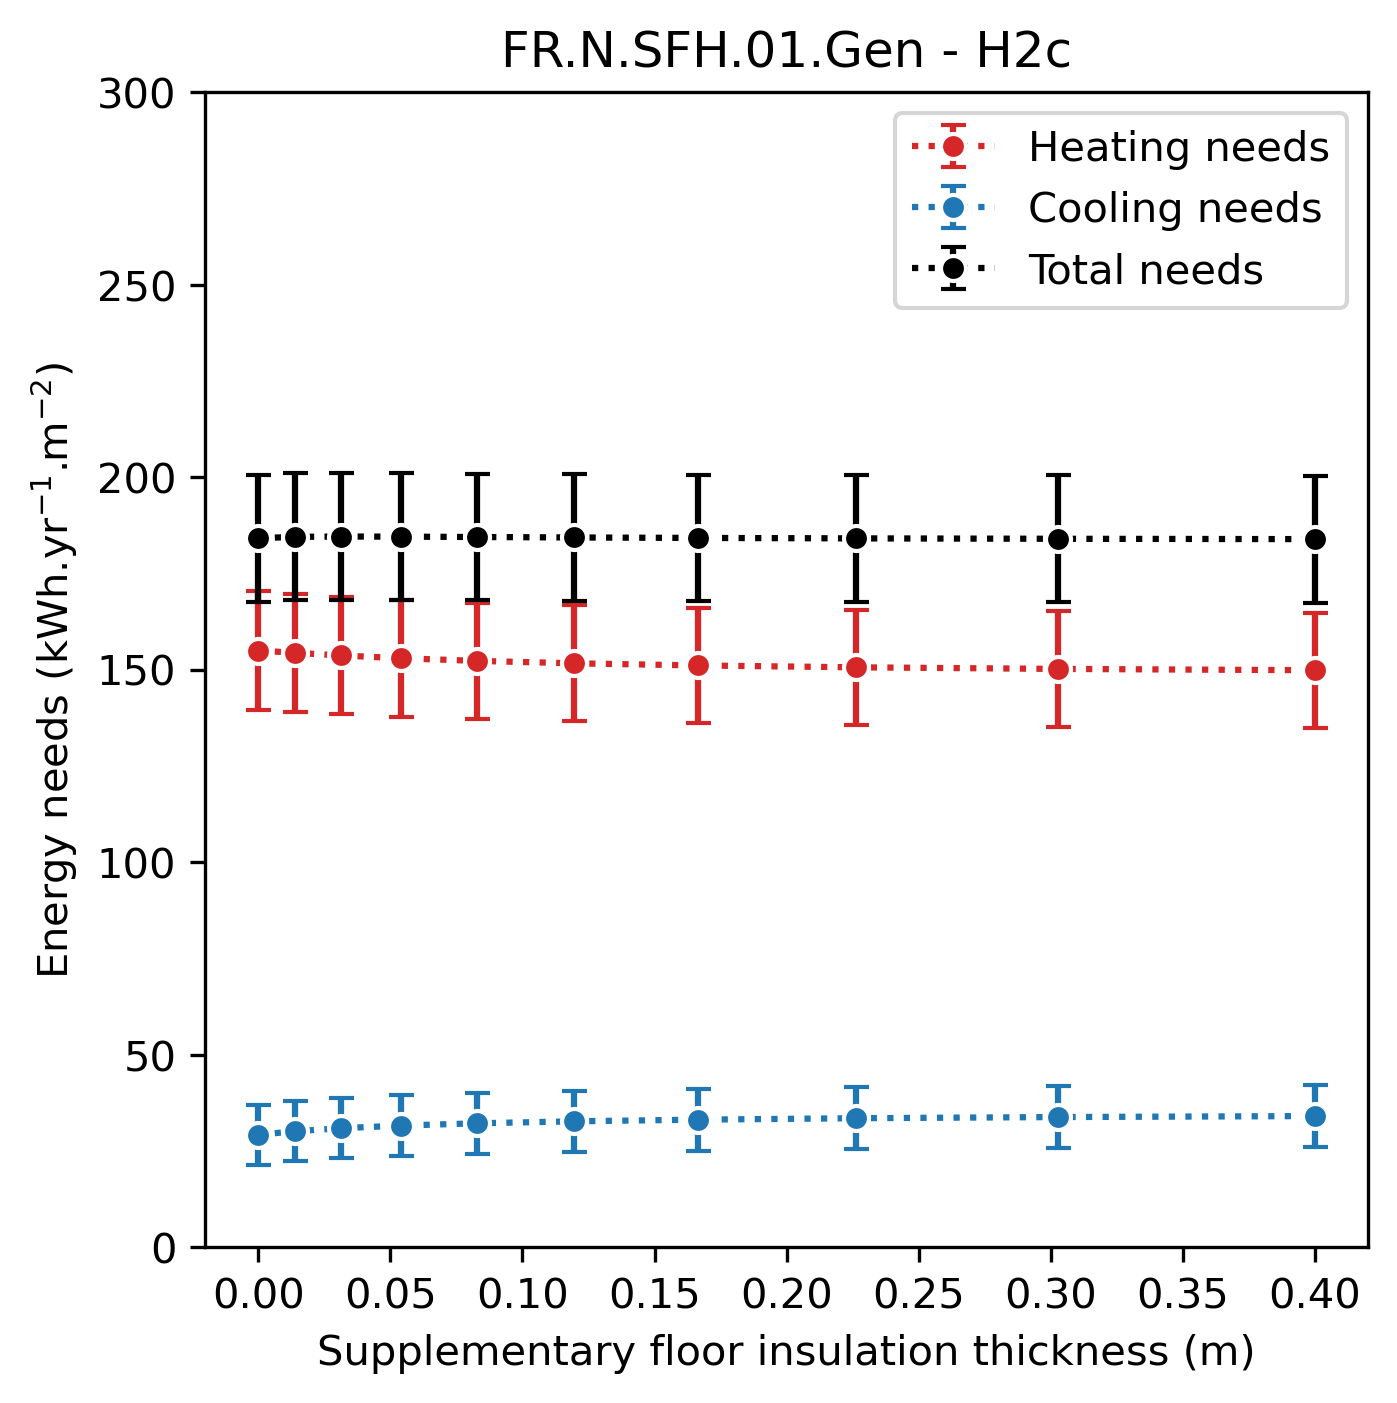
\includegraphics[width=0.32\columnwidth]{figures/floor_FR.N.SFH.01.Gen_H2c_conventionnel_th-bce_2020_2000-2020.png}
                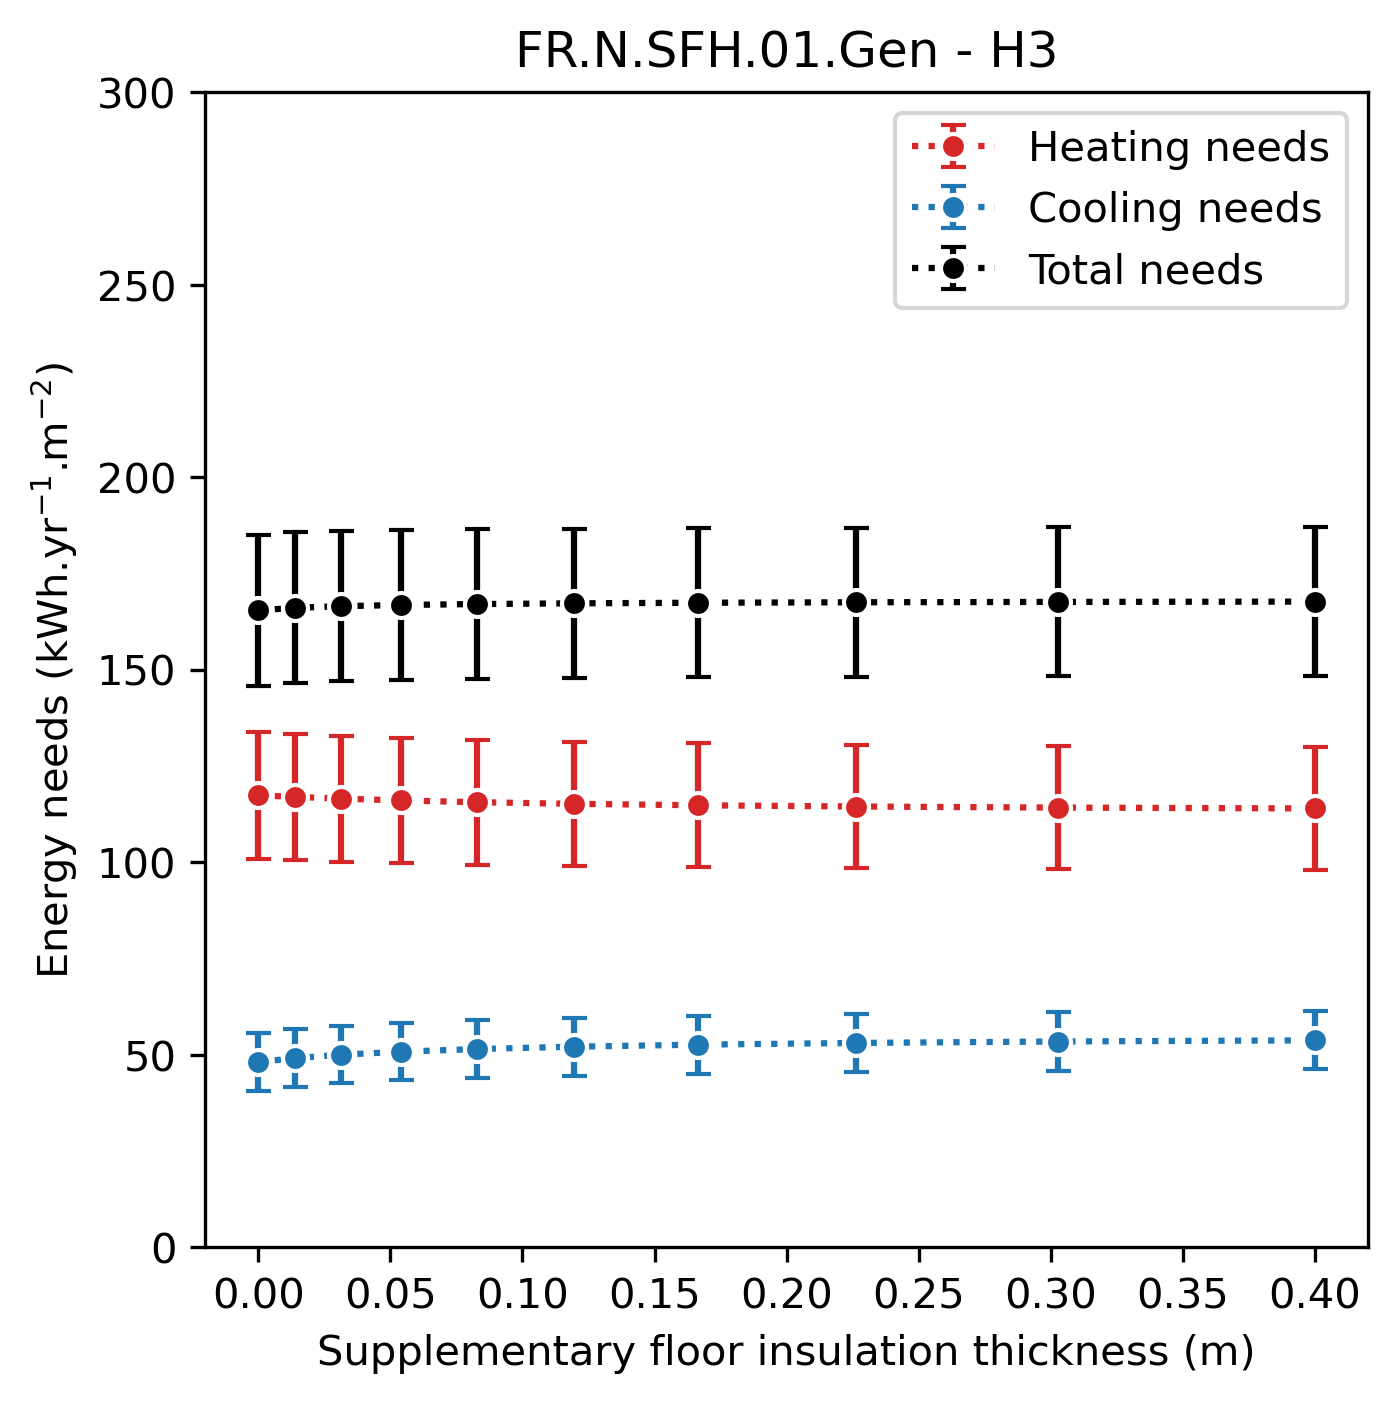
\includegraphics[width=0.32\columnwidth]{figures/floor_FR.N.SFH.01.Gen_H3_conventionnel_th-bce_2020_2000-2020.png}\\
                % 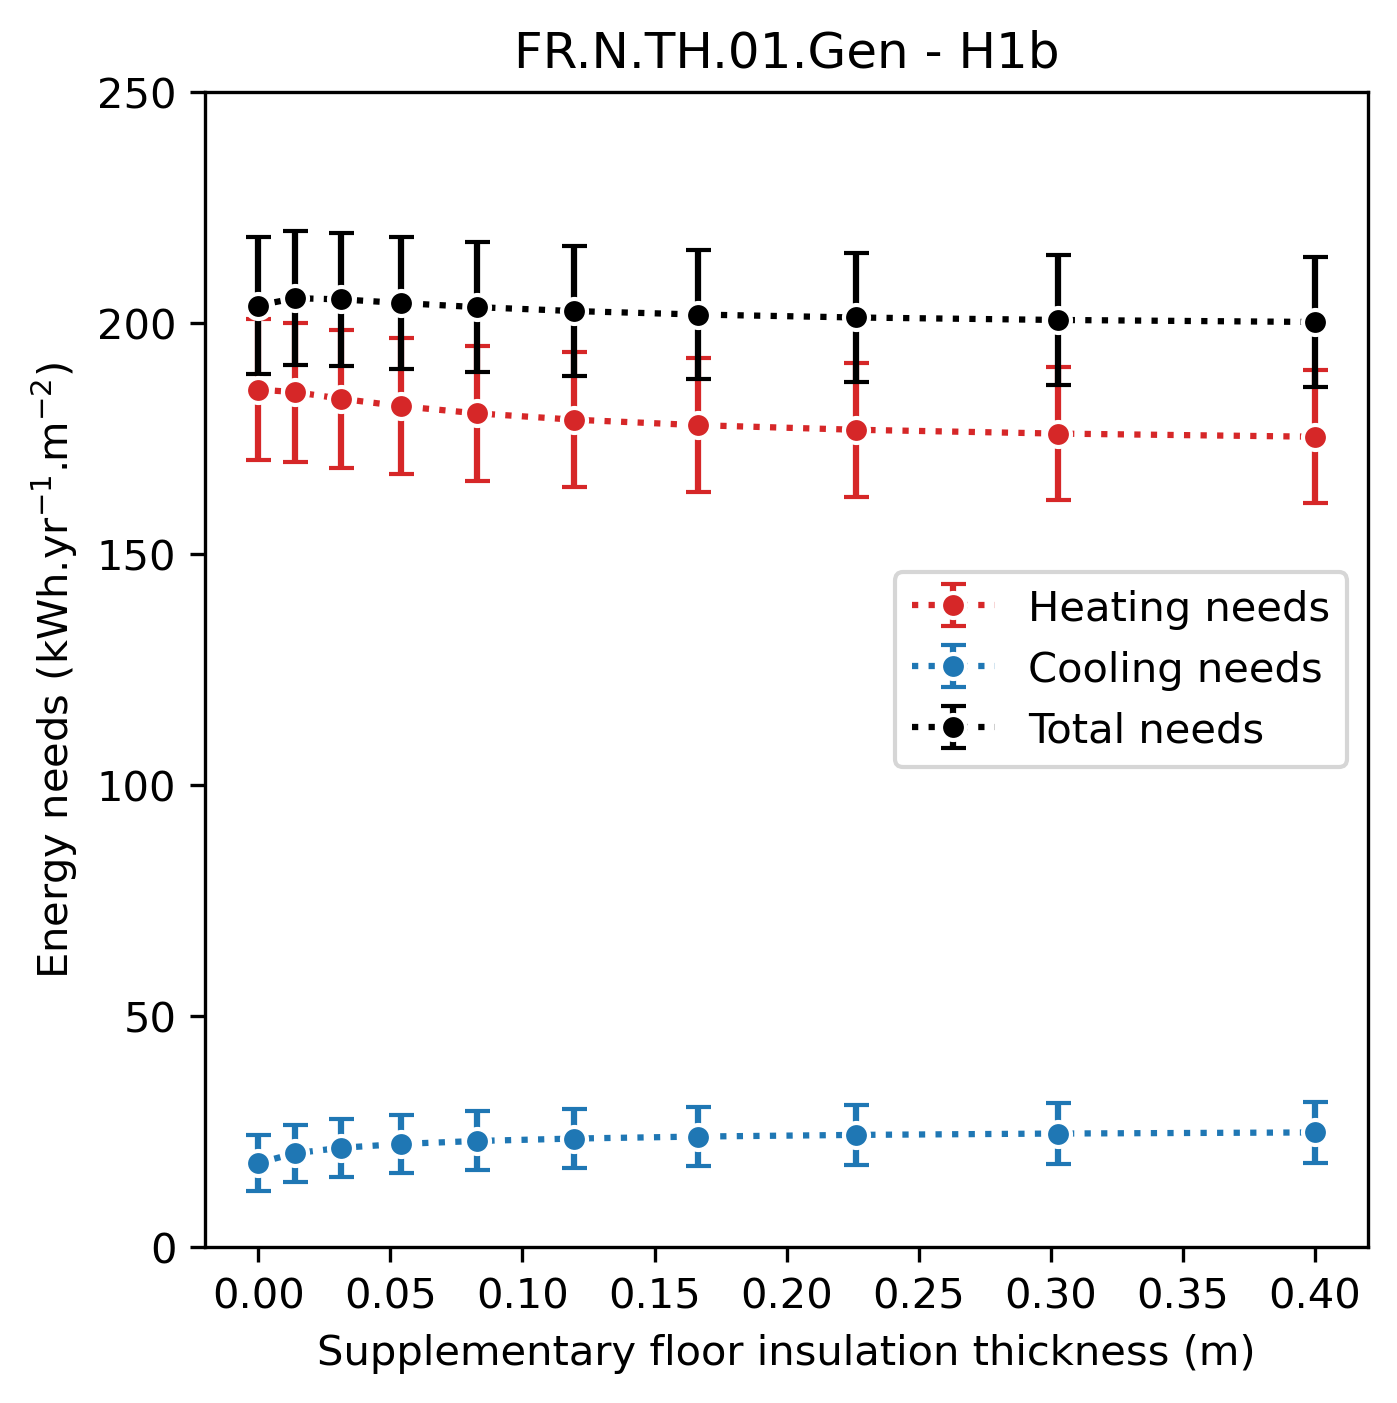
\includegraphics[width=0.32\columnwidth]{figures/floor_FR.N.TH.01.Gen_H1b_conventionnel_th-bce_2020_2000-2020.png}
                % 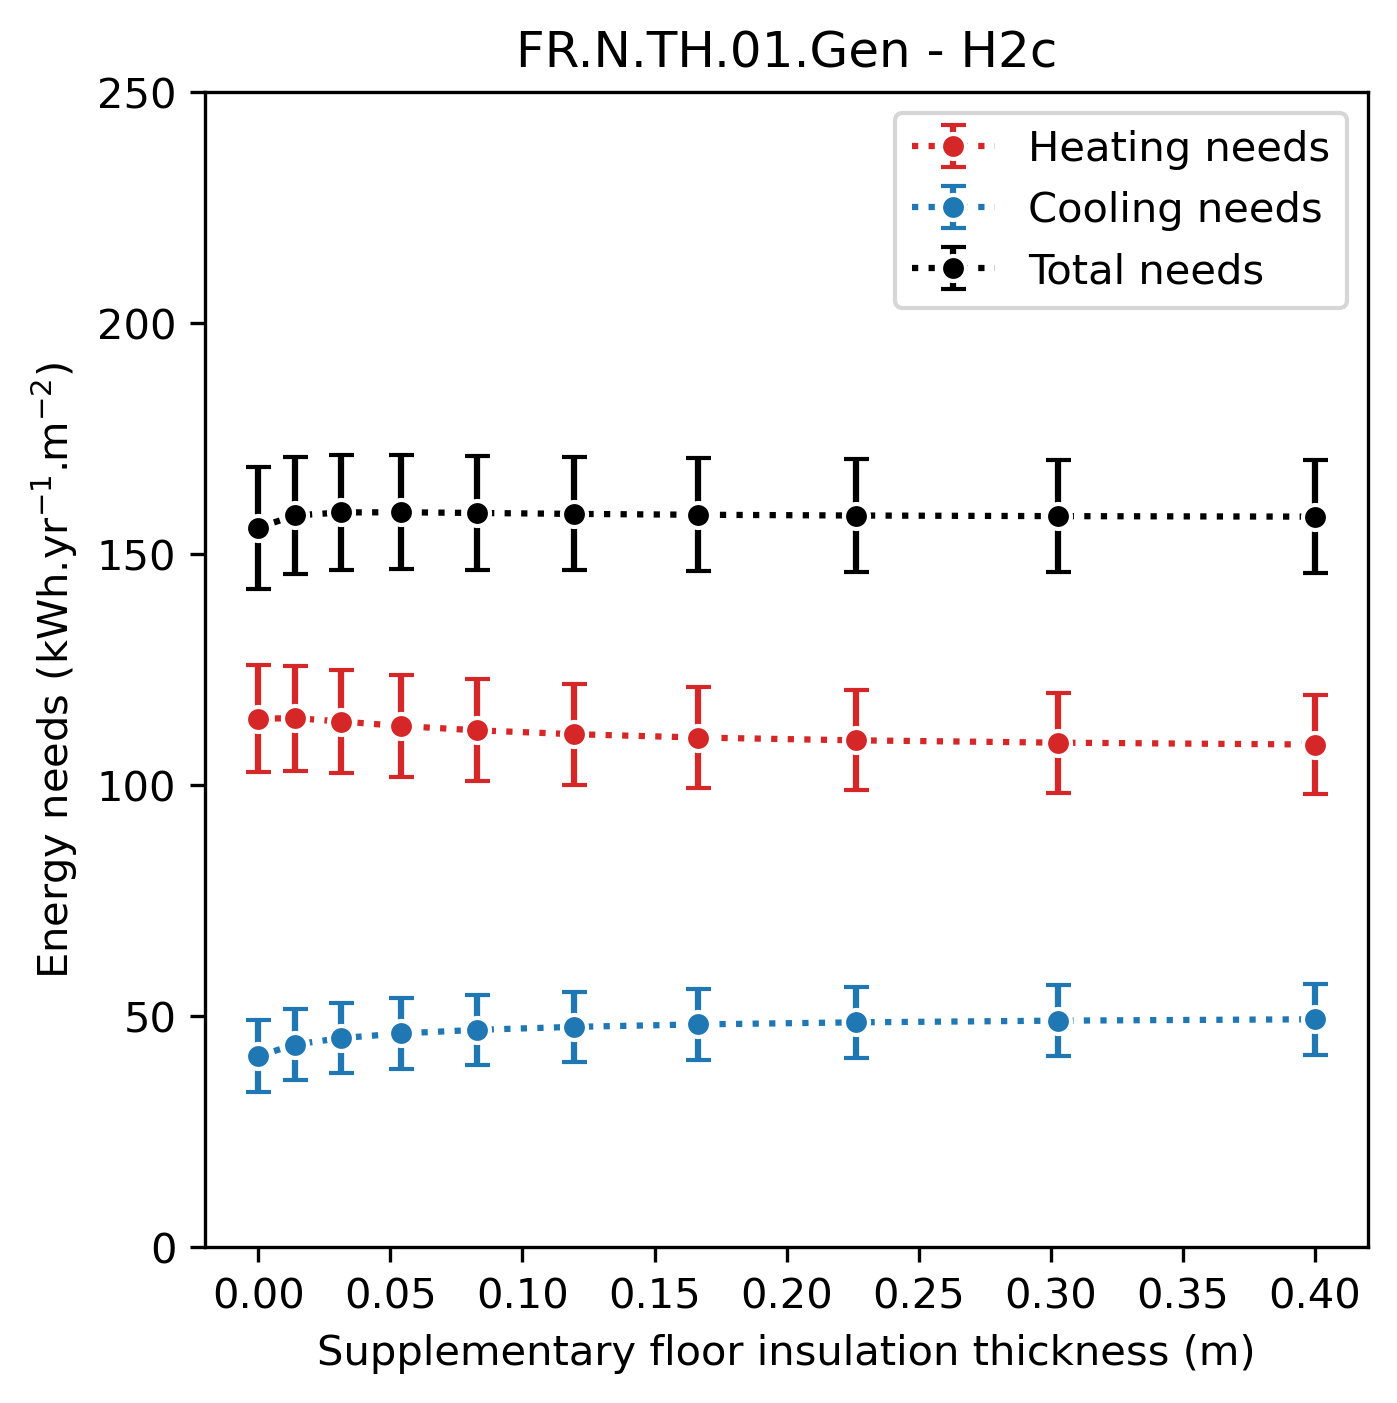
\includegraphics[width=0.32\columnwidth]{figures/floor_FR.N.TH.01.Gen_H2c_conventionnel_th-bce_2020_2000-2020.png}
                % 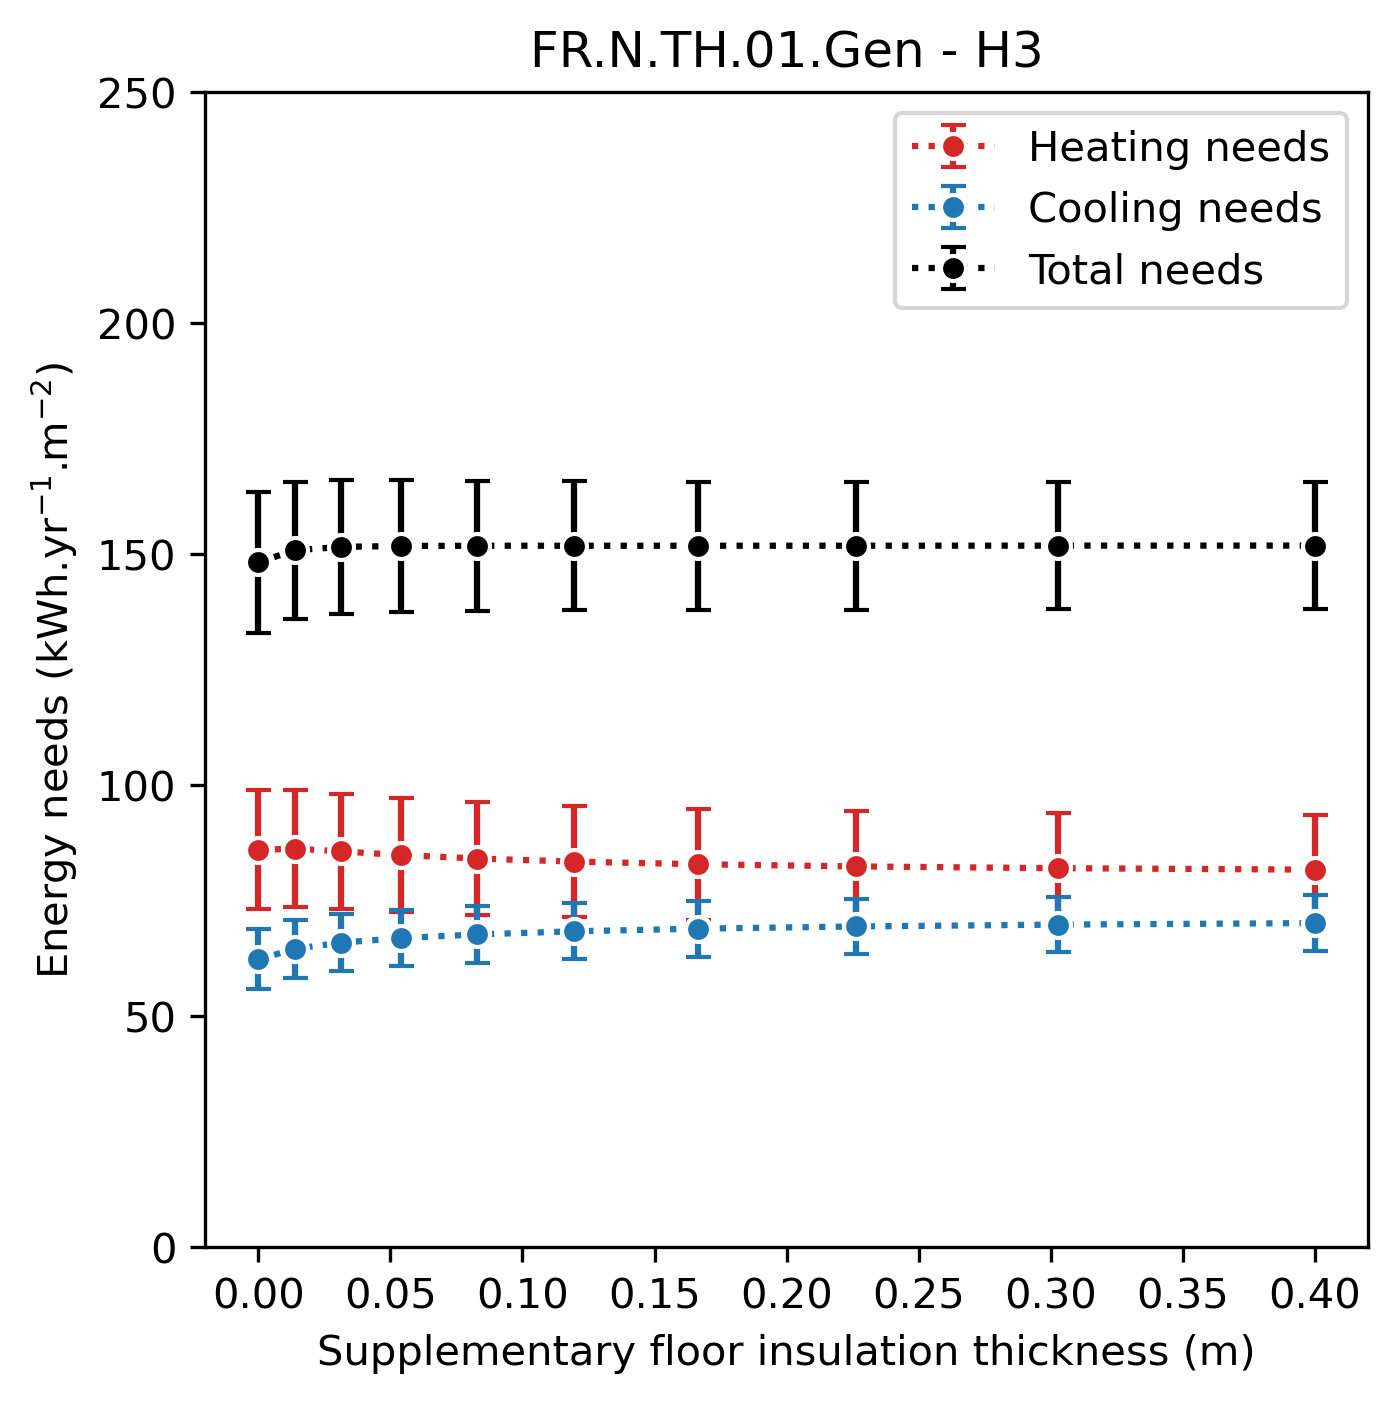
\includegraphics[width=0.32\columnwidth]{figures/floor_FR.N.TH.01.Gen_H3_conventionnel_th-bce_2020_2000-2020.png}\\
                % 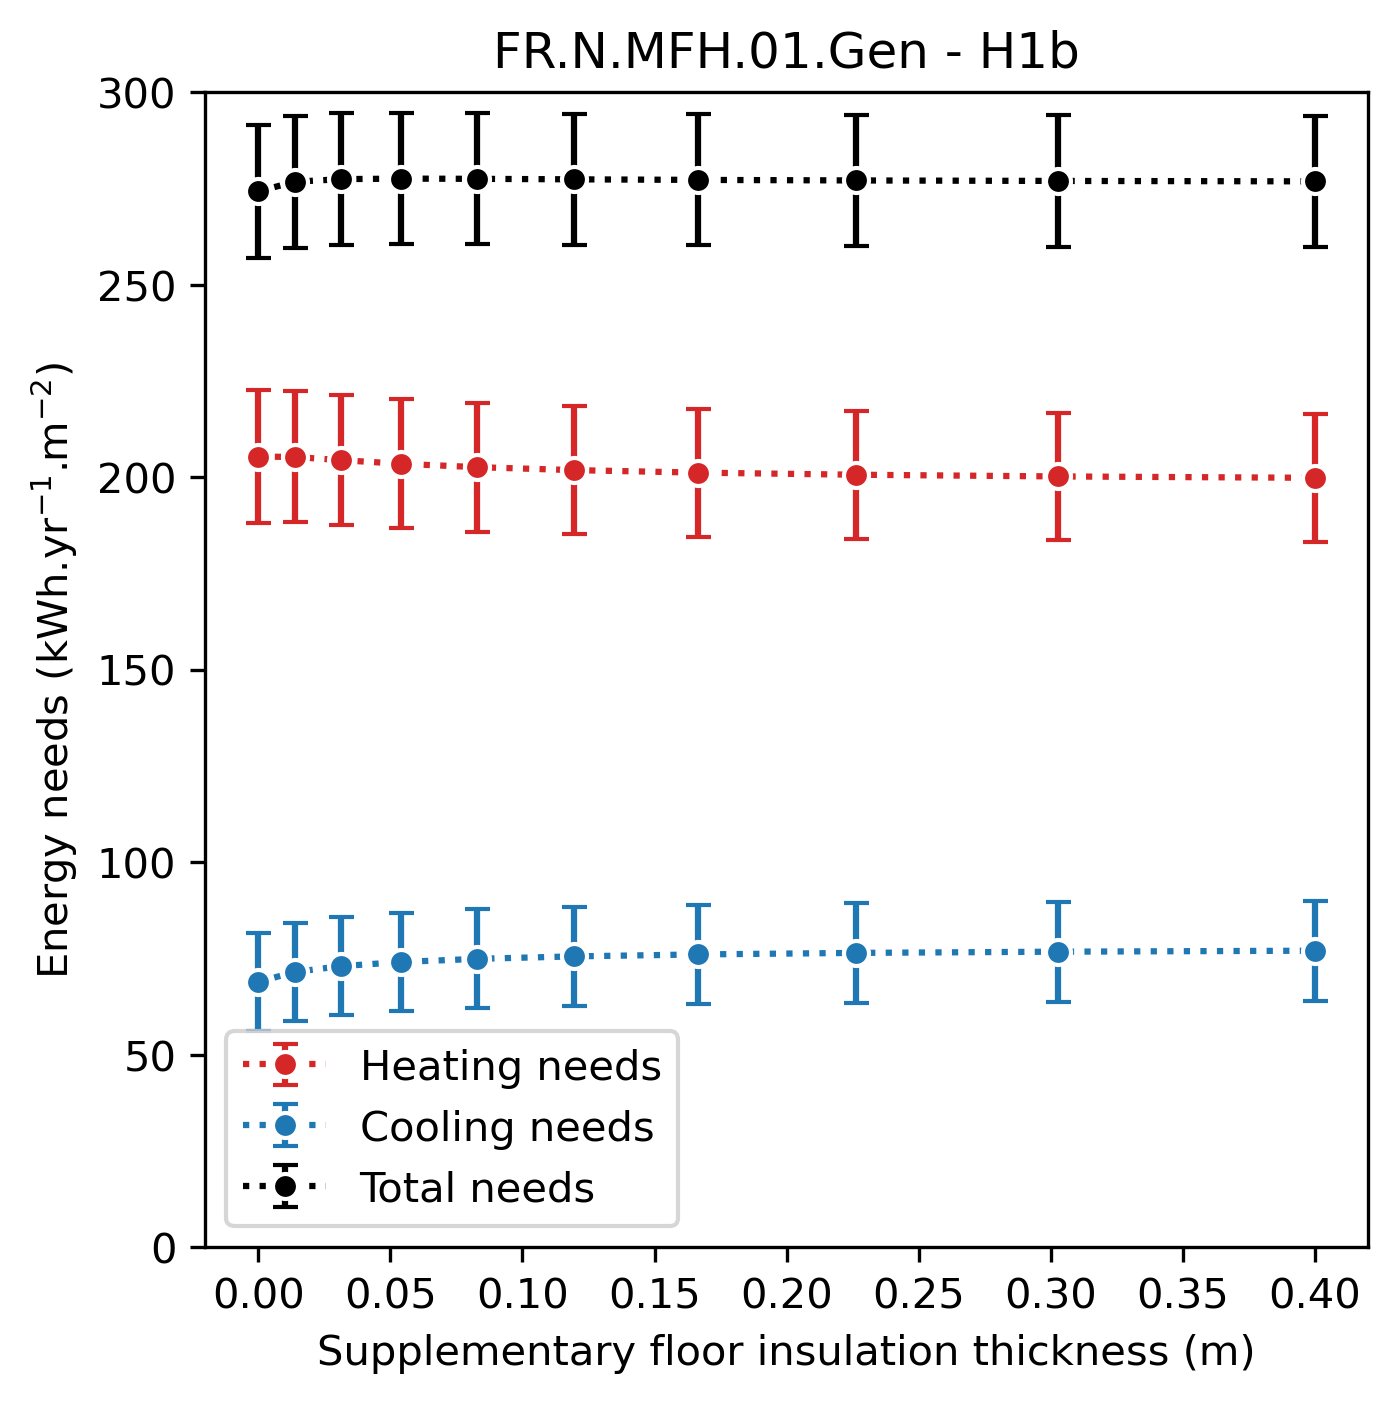
\includegraphics[width=0.32\columnwidth]{figures/floor_FR.N.MFH.01.Gen_H1b_conventionnel_th-bce_2020_2000-2020.png}
                % 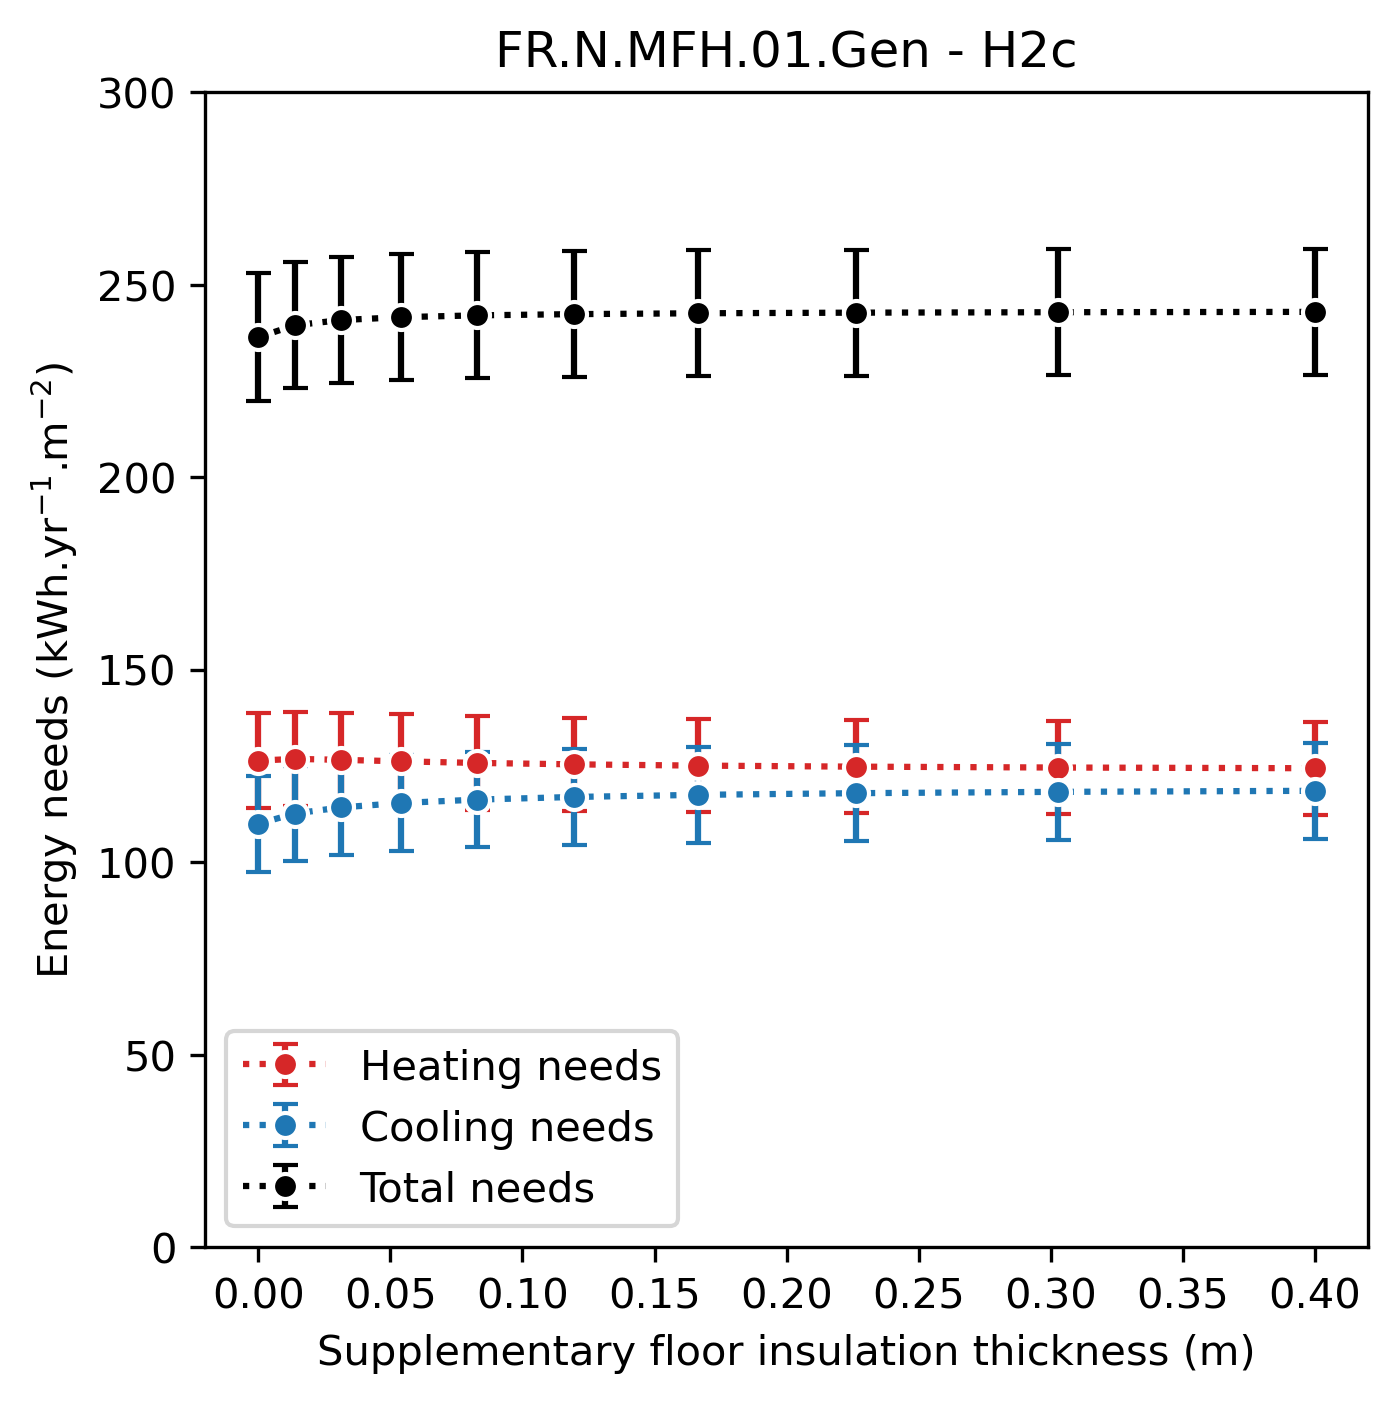
\includegraphics[width=0.32\columnwidth]{figures/floor_FR.N.MFH.01.Gen_H2c_conventionnel_th-bce_2020_2000-2020.png}
                % 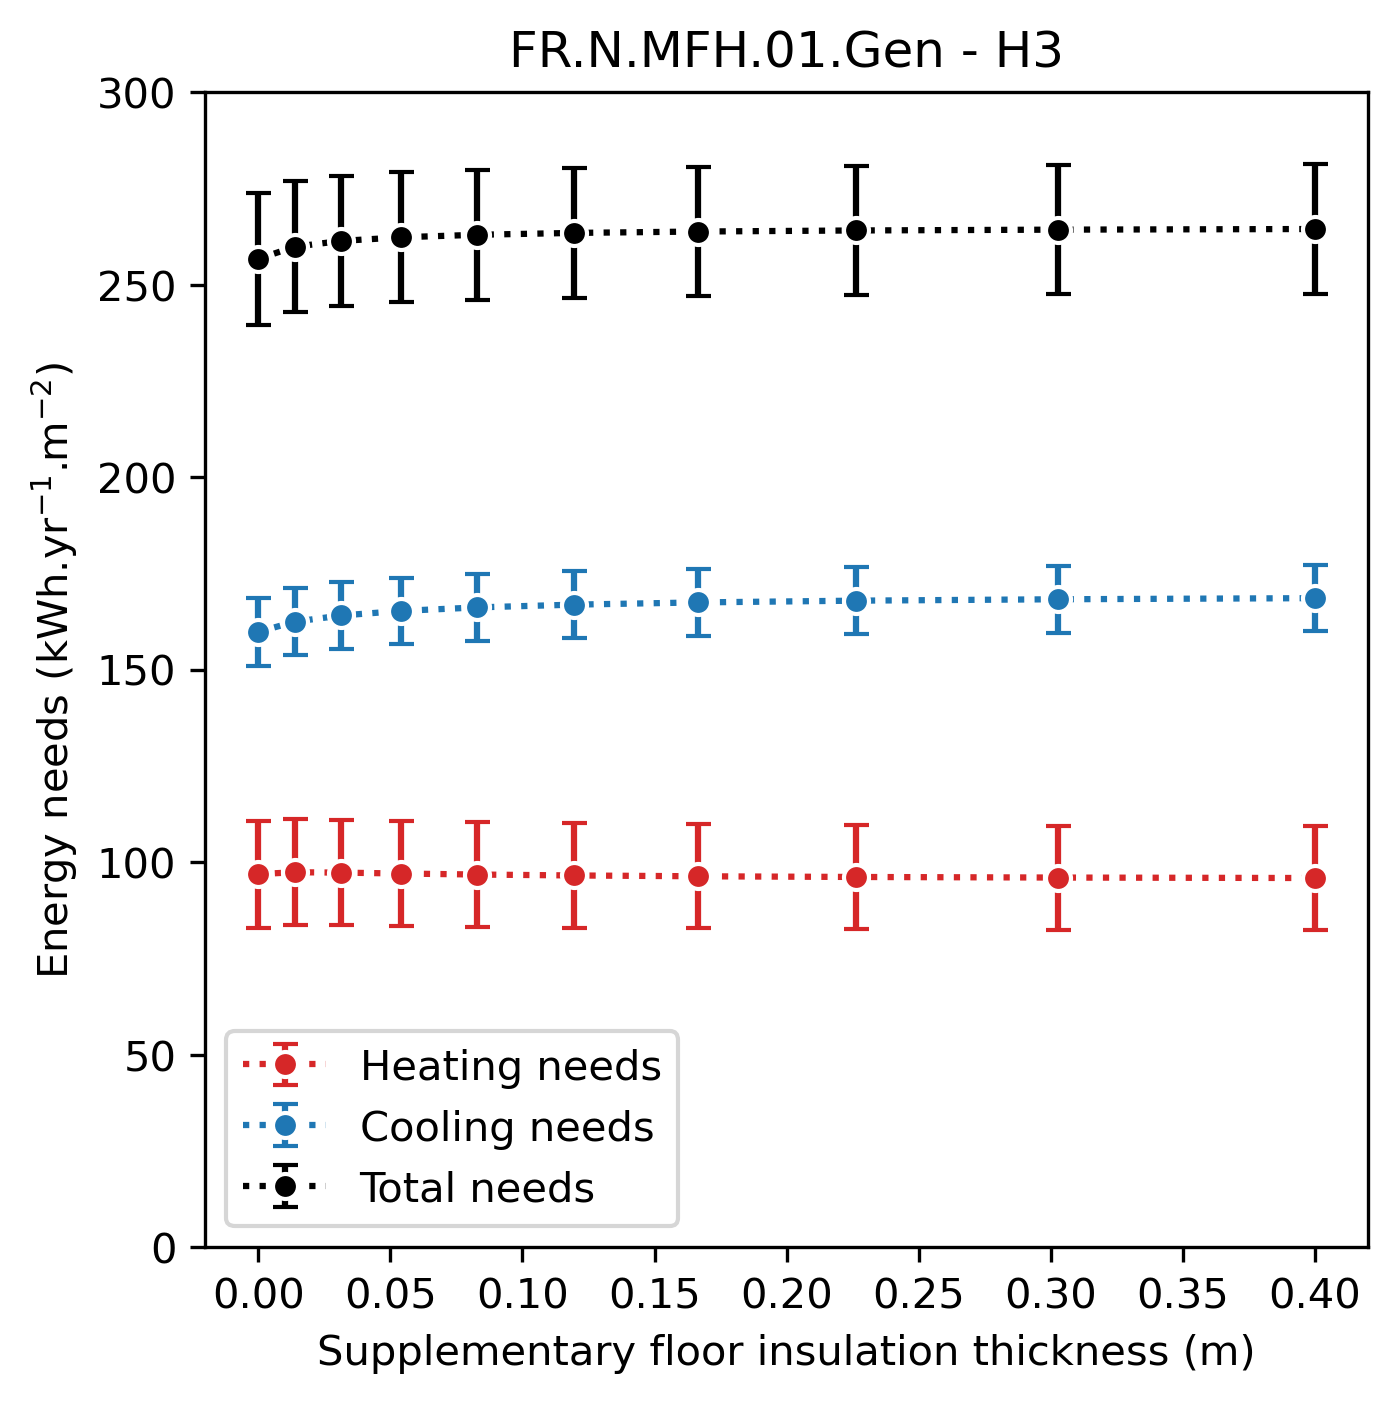
\includegraphics[width=0.32\columnwidth]{figures/floor_FR.N.MFH.01.Gen_H3_conventionnel_th-bce_2020_2000-2020.png}\\
                \includegraphics[width=0.32\columnwidth]{figures/floor_FR.N.AB.03.Gen_H1b_conventionnel_th-bce_2020_2000-2020.png}
                \includegraphics[width=0.32\columnwidth]{figures/floor_FR.N.AB.03.Gen_H2c_conventionnel_th-bce_2020_2000-2020.png}
                \includegraphics[width=0.32\columnwidth]{figures/floor_FR.N.AB.03.Gen_H3_conventionnel_th-bce_2020_2000-2020.png}
                \caption{\label{fig:floor_init} Effects of floor insulation thickness on energy needs.}
                \begin{quote}
                    \vspace{-2mm}
                    \small\noindent
                    \textbf{(left to right, top to bottom)} Description
                  \end{quote}
            \end{figure}
        
        % subsubsection floor_insulation (end)

        \subsubsection{Color of external surface} % (fold)
        \label{ssub:color_of_external_surface}

            processus physique à décrire

            detailler les interactions (\ref{fig:color_init})

            \begin{figure}[ht]
                \centering
                \includegraphics[width=0.32\columnwidth]{figures/albedo_FR.N.SFH.01.Gen_H1b_conventionnel_th-bce_2020_2000-2020.png}
                \includegraphics[width=0.32\columnwidth]{figures/albedo_FR.N.SFH.01.Gen_H2c_conventionnel_th-bce_2020_2000-2020.png}
                \includegraphics[width=0.32\columnwidth]{figures/albedo_FR.N.SFH.01.Gen_H3_conventionnel_th-bce_2020_2000-2020.png}\\
                % \includegraphics[width=0.32\columnwidth]{figures/albedo_FR.N.TH.01.Gen_H1b_conventionnel_th-bce_2020_2000-2020.png}
                % \includegraphics[width=0.32\columnwidth]{figures/albedo_FR.N.TH.01.Gen_H2c_conventionnel_th-bce_2020_2000-2020.png}
                % \includegraphics[width=0.32\columnwidth]{figures/albedo_FR.N.TH.01.Gen_H3_conventionnel_th-bce_2020_2000-2020.png}\\
                % \includegraphics[width=0.32\columnwidth]{figures/albedo_FR.N.MFH.01.Gen_H1b_conventionnel_th-bce_2020_2000-2020.png}
                % \includegraphics[width=0.32\columnwidth]{figures/albedo_FR.N.MFH.01.Gen_H2c_conventionnel_th-bce_2020_2000-2020.png}
                % \includegraphics[width=0.32\columnwidth]{figures/albedo_FR.N.MFH.01.Gen_H3_conventionnel_th-bce_2020_2000-2020.png}\\
                % \includegraphics[width=0.32\columnwidth]{figures/albedo_FR.N.AB.03.Gen_H1b_conventionnel_th-bce_2020_2000-2020.png}
                % \includegraphics[width=0.32\columnwidth]{figures/albedo_FR.N.AB.03.Gen_H2c_conventionnel_th-bce_2020_2000-2020.png}
                % \includegraphics[width=0.32\columnwidth]{figures/albedo_FR.N.AB.03.Gen_H3_conventionnel_th-bce_2020_2000-2020.png}
                \caption{\label{fig:color_init} Effects of external surface color on energy needs.}
                \begin{quote}
                    \vspace{-2mm}
                    \small\noindent
                    \textbf{(left to right)} Description
                  \end{quote}
            \end{figure}
        
        % subsubsection color_of_external_surface (end)

        \subsubsection{Ventilation efficiency} % (fold)
        \label{ssub:ventilation_efficiency}

            décrire les types de ventilation et leurs principales différences 

            mentionner le by pass et surventilation nocturne 

            detailler les interactions (\ref{fig:ventil_init})

            \begin{figure}[ht]
                \centering
                \includegraphics[width=0.32\columnwidth]{figures/ventilation_FR.N.SFH.01.Gen_H1b_conventionnel_th-bce_2020_2000-2020.png}
                \includegraphics[width=0.32\columnwidth]{figures/ventilation_FR.N.SFH.01.Gen_H2c_conventionnel_th-bce_2020_2000-2020.png}
                \includegraphics[width=0.32\columnwidth]{figures/ventilation_FR.N.SFH.01.Gen_H3_conventionnel_th-bce_2020_2000-2020.png}\\
                % \includegraphics[width=0.32\columnwidth]{figures/ventilation_FR.N.TH.01.Gen_H1b_conventionnel_th-bce_2020_2000-2020.png}
                % \includegraphics[width=0.32\columnwidth]{figures/ventilation_FR.N.TH.01.Gen_H2c_conventionnel_th-bce_2020_2000-2020.png}
                % \includegraphics[width=0.32\columnwidth]{figures/ventilation_FR.N.TH.01.Gen_H3_conventionnel_th-bce_2020_2000-2020.png}\\
                % \includegraphics[width=0.32\columnwidth]{figures/ventilation_FR.N.MFH.01.Gen_H1b_conventionnel_th-bce_2020_2000-2020.png}
                % \includegraphics[width=0.32\columnwidth]{figures/ventilation_FR.N.MFH.01.Gen_H2c_conventionnel_th-bce_2020_2000-2020.png}
                % \includegraphics[width=0.32\columnwidth]{figures/ventilation_FR.N.MFH.01.Gen_H3_conventionnel_th-bce_2020_2000-2020.png}\\
                % \includegraphics[width=0.32\columnwidth]{figures/ventilation_FR.N.AB.03.Gen_H1b_conventionnel_th-bce_2020_2000-2020.png}
                % \includegraphics[width=0.32\columnwidth]{figures/ventilation_FR.N.AB.03.Gen_H2c_conventionnel_th-bce_2020_2000-2020.png}
                % \includegraphics[width=0.32\columnwidth]{figures/ventilation_FR.N.AB.03.Gen_H3_conventionnel_th-bce_2020_2000-2020.png}
                \caption{\label{fig:ventil_init} Effects of ventilation system on energy needs.}
                \begin{quote}
                    \vspace{-2mm}
                    \small\noindent
                    \textbf{(left to right)} Description
                \end{quote}
            \end{figure}
        
        % subsubsection ventilation_efficiency (end)

        \subsubsection{Shading of glazed surfaces} % (fold)
        \label{ssub:shading_of_glazed}

        description des travaux, cf schéma 

        detailler les interactions (\ref{fig:shading_init})

        importance des volets et des comportements associés 

        \begin{figure}[ht]
            \centering
            % \includegraphics[width=0.32\columnwidth]{figures/shading_FR.N.SFH.01.Gen_H1b_conventionnel_th-bce_2020_2000-2020.png}
            % \includegraphics[width=0.32\columnwidth]{figures/shading_FR.N.SFH.01.Gen_H2c_conventionnel_th-bce_2020_2000-2020.png}
            % \includegraphics[width=0.32\columnwidth]{figures/shading_FR.N.SFH.01.Gen_H3_conventionnel_th-bce_2020_2000-2020.png}\\
            \includegraphics[width=0.32\columnwidth]{figures/shading_FR.N.TH.01.Gen_H1b_conventionnel_th-bce_2020_2000-2020.png}
            \includegraphics[width=0.32\columnwidth]{figures/shading_FR.N.TH.01.Gen_H2c_conventionnel_th-bce_2020_2000-2020.png}
            \includegraphics[width=0.32\columnwidth]{figures/shading_FR.N.TH.01.Gen_H3_conventionnel_th-bce_2020_2000-2020.png}\\
            % \includegraphics[width=0.32\columnwidth]{figures/shading_FR.N.MFH.01.Gen_H1b_conventionnel_th-bce_2020_2000-2020.png}
            % \includegraphics[width=0.32\columnwidth]{figures/shading_FR.N.MFH.01.Gen_H2c_conventionnel_th-bce_2020_2000-2020.png}
            % \includegraphics[width=0.32\columnwidth]{figures/shading_FR.N.MFH.01.Gen_H3_conventionnel_th-bce_2020_2000-2020.png}\\
            % \includegraphics[width=0.32\columnwidth]{figures/shading_FR.N.AB.03.Gen_H1b_conventionnel_th-bce_2020_2000-2020.png}
            % \includegraphics[width=0.32\columnwidth]{figures/shading_FR.N.AB.03.Gen_H2c_conventionnel_th-bce_2020_2000-2020.png}
            % \includegraphics[width=0.32\columnwidth]{figures/shading_FR.N.AB.03.Gen_H3_conventionnel_th-bce_2020_2000-2020.png}
            \caption{\label{fig:shading_init} Effects of solar protection length over windows on energy needs.}
            \begin{quote}
                \vspace{-2mm}
                \small\noindent
                \textbf{(left to right)} Description
            \end{quote}
        \end{figure}
        
        % subsubsection shading_of_ (end)
    % subsection characterisation_of_single_renovation_actions (end)    

    \subsection{Energy needs for TABULA typologies} % (fold)
    \label{sub:energy_needs_for_tabula_typologies}

        \subsubsection{Single Family House (SFH)} % (fold)
        \label{ssub:sfh}

        detailler les résultats (\ref{fig:sfh_needs})
        
        \begin{figure}[ht]
            \centering
            \includegraphics[width=0.49\columnwidth]{figures/typology_energy_needs_SFH_H1b_2000-2020.png}
            \includegraphics[width=0.49\columnwidth]{figures/typology_energy_needs_SFH_H3_2000-2020.png}
            \caption{\label{fig:sfh_needs} Heating and cooling needs for SFH typologies.}
            \begin{quote}
                \vspace{-2mm}
                \small\noindent
                \textbf{(left to right)} Description
            \end{quote}
        \end{figure}

        % subsubsection sfh (end)

        \subsubsection{Terraced House (TH)} % (fold)
        \label{ssub:th}

        detailler les résultats (\ref{fig:th_needs})

        \begin{figure}[ht]
            \centering
            \includegraphics[width=0.49\columnwidth]{figures/typology_energy_needs_TH_H1b_2000-2020.png}
            \includegraphics[width=0.49\columnwidth]{figures/typology_energy_needs_TH_H3_2000-2020.png}
            \caption{\label{fig:th_needs} Heating and cooling needs for TH typologies.}
            \begin{quote}
                \vspace{-2mm}
                \small\noindent
                \textbf{(left to right)} Description
            \end{quote}
        \end{figure}
        
        % subsubsection th (end)

        \subsubsection{Multi Family House (MFH)} % (fold)
        \label{ssub:mfh}
        
        detailler les résultats (\ref{fig:mfh_needs})

        \begin{figure}[ht]
            \centering
            \includegraphics[width=0.49\columnwidth]{figures/typology_energy_needs_MFH_H1b_2000-2020.png}
            \includegraphics[width=0.49\columnwidth]{figures/typology_energy_needs_MFH_H3_2000-2020.png}
            \caption{\label{fig:mfh_needs} Heating and cooling needs for MFH typologies.}
            \begin{quote}
                \vspace{-2mm}
                \small\noindent
                \textbf{(left to right)} Description
            \end{quote}
        \end{figure}

        % subsubsection mfh (end)

        \subsubsection{Appartment Block (AB)} % (fold)
        \label{ssub:ab}

        detailler les résultats (\ref{fig:ab_needs})
        
        \begin{figure}[ht]
            \centering
            \includegraphics[width=0.49\columnwidth]{figures/typology_energy_needs_AB_H1b_2000-2020.png}
            \includegraphics[width=0.49\columnwidth]{figures/typology_energy_needs_AB_H3_2000-2020.png}
            \caption{\label{fig:ab_needs} Heating and cooling needs for AB typologies.}
            \begin{quote}
                \vspace{-2mm}
                \small\noindent
                \textbf{(left to right)} Description
            \end{quote}
        \end{figure}

        % subsubsection ab (end)
        
    % subsection energy_needs_for_tabula_typologies (end)
% section inter (end)

\clearpage
\section{Climate impact on optimal renovations}
\label{sec:opti}

    \subsection{Optimal energy efficiency} % (fold)
    \label{sub:optimal_energy_efficiency}
    
    % subsection optimal_energy_efficiency (end)

    \subsection{Optimal economic efficiency} % (fold)
    \label{sub:optimal_economic_efficiency}
    
    % subsection optimal_economic_efficiency (end)
% section opti (end)

\clearpage
\section{Generalisation across the whole French building stock}
\label{sec:generalisation}
    
    \subsection{Building stock calibration} % (fold)
    \label{sub:calibration}
    
    utilisation de la base DPE (statistiques)

    description de la représentatitivté de la base DPE (BDNB) (\ref{fig:epc})

    \begin{figure}[ht]
        \centering
        \includegraphics[width=0.32\columnwidth]{figures/carte_repr_maison_dpe_nblog-BDNB.png}
        \includegraphics[width=0.32\columnwidth]{figures/carte_repr_appartement_dpe_nblog-BDNB.png}
        \includegraphics[width=0.32\columnwidth]{figures/DPE_distribution_dpe_france.png}
        \caption{\label{fig:epc} Representativeness of EPC data in terms of number of dwellings and in energy performance labels.}
        \begin{quote}
            \vspace{-2mm}
            \small\noindent
            \textbf{(left to right)} Representativeness maps for single-family homes (SFH + TH) and multi-family homes (MFH + AB), and comparison of the distribution of energy performance labels in France (\cite{onre_parc_2022}) and in the BDNB database. Data from the BDNB (\cite{cstb_base_2024}), version 2023-11-a, aggregating data from the DPE database and the property database (\cite{ademe_donnees_2024}, \cite{cerema_documentation_2024}). 
        \end{quote}
    \end{figure}
    % subsection calibration (end)

    \subsection{Projection of heating and cooling needs} % (fold)
    \label{sub:evolution_des_besoins_énergétiques}
    
    % subsection evolution_des_besoins_énergétiques (end)

    \subsection{Projection of annual and instant energy demand} % (fold)
    \label{sub:évoltuion_des_consommations}
    
    % subsection évoltuion_des_consommations (end)
% section generalisation (end)

\clearpage
\section{Discussion}
\label{sec:disc}
% section disc (end)

\clearpage
\section{Conclusion}
\label{sec:conclu}
% section conclu (end)



\clearpage
\printbibliography


\appendix

\clearpage
\section{Appendix} % (fold)
\label{sec:appendix}

    \subsection{Effects of time resolution on energy and power needs} % (fold)
    \label{sub:effects_of_time_resolution_on_energy_and_power_needs}
    
    % subsection effects_of_time_resolution_on_energy_and_power_needs (end)

    \subsection{U-values comparison with TABULA typologies} % (fold)
    \label{sub:u_values_comparison_with_tabula_typologies}
    
    % subsection u_values_comparison_with_tabula_typologies (end)
    
    \subsection{Single renovation actions on initial typologies} % (fold)
    \label{sub:single_renovation_actions_on_initial_typologies}
    
    % subsection single_renovation_actions_on_initial_typologies (end)

% section appendix (end)


\end{document}